\documentclass[journal]{IEEEtran}

\pagestyle{plain}

\usepackage[english,american]{babel}
\usepackage{graphicx}
\usepackage{subfigure}
\usepackage{amsmath}
\usepackage{multirow}
\usepackage{multicol}
\usepackage{float}
\usepackage{algorithm}
\usepackage{algorithmic}
\usepackage[colorlinks, linkcolor=black, anchorcolor=black, citecolor=blue]{hyperref}
\usepackage{cite}
\usepackage{balance}
\usepackage{color}
\usepackage[square,sort,comma,numbers]{natbib}
\usepackage{url}
\usepackage{diagbox}
\usepackage{enumerate}
\usepackage{setspace}
\usepackage{enumitem}
\usepackage{indentfirst}
\usepackage{booktabs}
\usepackage{tikz}
\usepackage{listings}
\usepackage{etoolbox}
\usepackage{setspace}



\renewcommand{\algorithmicrequire}{\textbf{Input:}}
\renewcommand{\algorithmicensure}{\textbf{Output:}}
%\usepackage{setspace}
%\usepackage{epsfig,graphics,subfigure,psfrag,amsmath,amssymb}
\newcommand\FIXME[1]{\textcolor{red}{FIX:}\textcolor{red}{#1}}
\newcommand\FIXED[1]{\textcolor{blue}{FIXED: }\textcolor{blue}{#1}}


\newcommand{\circled}[2][]{\tikz[baseline=(char.base)]
    {\node[shape = circle, draw, inner sep = 1pt]
    (char) {\phantom{\ifblank{#1}{#2}{#1}}};%
    \node at (char.center) {\makebox[0pt][c]{#2}};}}
\robustify{\circled}

\begin{document}

\title{Video-side Channel Attack for Pattern Lock}


\author{Guixin Ye, Zhanyong Tang, Dingyi Fang, Xiaojiang Chen,
        Willy Wolf and Zheng Wang
\thanks{G. Ye, Z. Tang, D. Fang, and X. Chen are with Northwest University, China}%
\thanks{Willy Wolf and Zheng Wang are with Lancaster University, U.K.}
\thanks{
Extension of Conference Paper: a preliminary version of this article entitled ``Cracking Android Pattern Lock
in Five Attempts" by G. Ye, Z. Tang, D. Fang, X. Chen, K. Kim, B. Taylor and Z. Wang appeared in
The Network and Distributed System Security Symposium (NDSS) 2017~\cite{ye2017cracking}. 
The extended version makes the following several additional contributions over the conference
paper: \FIXME{bla bla...}
}
}


% The paper headers
\markboth{IEEE Transactions on Information Forensics and Security}%
{Ye \MakeLowercase{\textit{et al.}}: Video-side Channel Attack for Android Pattern Lock}

% make the title area
\maketitle

% As a general rule, do not put math, special symbols or citations
% in the abstract or keywords.
\begin{abstract}
    Pattern lock is widely used as a mechanism for authentication and authorization on Android devices. This paper presents a novel video-based attack to reconstruct Android lock patterns from video footage filmed using a mobile phone camera. Unlike prior attacks on pattern lock, our approach does not require the video to capture ant content displayed on the screen. Instead, we employ a computer vision algorithm to track the fingertip movements to infer the pattern. Using the geometry information extracted from the tracked fingertip motions, our approach is able to accurately identify a small number of (often one) candidate patterns to be tested by an adversary. We thoroughly evaluated our approach using 120 unique patterns collected from 215 independent users, by applying it to reconstruct patterns from video footage filmed using mobile phone cameras. Experimental results show that our approach can break over 95\% of the patterns in five attempts before the device is automatically locked by the Android operating system. We discovered that, in contrast to many people's belief, complex patterns do not offer stronger protection under our attacking scenarios. This is demonstrated by the fact that we are able to break all but one complex patterns as opposed to 60\%of the simple patterns in the first attempt. Since our threat model is common in day-to-day life, this paper calls for the community to revisit the risks of using Android pattern lock to protect sensitive information.
\end{abstract}

% Note that keywords are not normally used for peerreview papers.
\begin{IEEEkeywords}
    Pattern lock, Fingertip movement, Video-based attack, Sensitive information.
\end{IEEEkeywords}

\section{Introduction\label{sec:intro}}

%\begin{figure}[!htbp]
%    \centering
%    \includegraphics[height=5cm]{fig/1.pdf}
%    \caption{The distribution of the number of the graphical passwords.}
%\end{figure}

Pattern lock is widely used on Android devices to protect sensitive information. It is preferred by some users over PIN- or text-based
passwords, as psychology studies show that the human brain remembers and
recalls visual information better than numbers and
letters~\cite{DeAngeli:2005:PRW:1090412.1090419}.
According to a recent study, 40\% of the Android users
use patterns to protect their devices instead of a PIN~\cite{androidstudy}.
Pattern lock is also used for authentication. For example, \texttt{Alipay}, the largest
third-party online-payment platform, uses pattern lock as part of the login authentication.
Given its pervasive usage, a security breach of the pattern lock could lead to serious consequences.


Researchers have uncovered a number of ways to crack Android pattern lock.
Smudge attacks use the oily residues  left on the screen to recover
the pattern~\cite{aviv2010smudge}. However, this approach relies on the persistence of
the smudge which can be easily destroyed by subsequent on-screen activities after unlocking. In a recent study, Zhang
\emph{et al.}~\cite{zhang2016privacy} shows that it is possible to infer a locking pattern by analyzing how the WiFi signal is affected by the finger motions when drawing the pattern. Their approach is restricted to
a limit set of scenarios due to two reasons: (1) the complex setup of the attacking environment and (2) the WiFi signal can be disrupted by any moving
objects nearby or body movements.


Recently, video-based side-channel attacks are shown to be effective in reconstructing PIN- or
text-based passwords. Some of the early works in this area rely on video
footage filmed using a camera directly facing the screen or the keyboard~\cite{
kuhn2002compromising, balzarotti2008clearshot}. Recent works show that
this limit can be lifted by exploiting spatial-temporal dynamics of
the hands during typing~\cite{shukla2014beware}.
Despite the success of
video-based attacks on PIN- and text-based passwords, no work so far has
exploited video-based side-channels to crack pattern lock.
To do so, the attack must address several new challenges. These include: How to map the user's fingertip
movements to a graphical structure consisting of continuous points instead of discrete
keystrokes? How to transform the fingertip movements tracked from
the camera's perspective to the user's view point to correctly reconstruct the
pattern? How to cancel the camera shake effect that can significantly
affect the performance of the attack? How to identify two overlapping line segments
of a pattern? The size of the touch-screen or the pattern grid
can vary from one device or one application to the other, how can the algorithm
adapt to these changes?
These new challenges make prior work video-based attacks inapplicable.
To overcome these challenges requires creative
solutions to be constructed in the new application context of pattern lock.

%This is fundamentally
%different from a PIN or a text-based password consisting of discrete
%characters. Therefore, those techniques proposed in prior research on PIN-
%and text-based password attacks is not directly applicable to extract lock
%patterns from video footage.

%\FIXED{Considering its widely usage, pattern lock has already attracted
%attacker's attention. Researchers have proposed some attacks on Android
%pattern lock~\cite{aviv2010smudge,zhang2016privacy}. Among these attacks,
%Adam proposes a smudge attack by filming the image that contains the residual
%smudges after drawing the pattern lock~\cite{aviv2010smudge}. Such method,
%however, have a strong assumption that the attacker need to have the
%possession of the device for full controlling the lighting and camera
%condition to extract the smudgy information of pattern lock. Zhang proposes
%an attacking approach that can snoop the pattern lock by leveraging the
%impact of finer movement on the Wi-Fi signal while drawing the
%pattern~\cite{zhang2016privacy}. However, such approach is limited to the
%complex scenarios as other moving objects will greatly
%disturb the excepted Wi-Fi signal, making this approach perform poor in practical scenarios.}

%Computer vision based attacks have emerged as a new way of attacking
%text-based passwords on touched screen systems. \FIXED{Prior works have} made use of
%reflection of objects to reconstruct what the user types on the touched
%screen to recover the
%password~\cite{kuhn2002compromising,xu2013seeing,raguram2011ispy,backes2009tempest}.
%The previous methods relies on the use of a digital single-lens reflex (DSLR)
%camera to film the content of user input (e.g., chats, username, passwords),
%making this kind of attack easy to be found. Shukla et al. leverage the
%spatio-temporal dynamic of the hands to infer the pin based passwords
%\cite{shukla2014beware}. Similarly, Yue et al. identify the pin based
%passwords by light diffusion surrounding touched keys \cite{yue2014blind}.
%However, such attacking schemes need to know the layout of the keyboard (such
%as the size of each key and the location of each key on the keypad). Such
%assumptions, however, do not hold for pattern hock, making the prior work
%infeasible for attacking
%pattern-based lock.

This paper presents a novel approach to crack Android pattern lock using
video footage that captures the user's fingertip motions when drawing the pattern. Unlike smudge attacks~\cite{aviv2010smudge}, our approach
does not require the video footage or images to be captured by a camera
directly faced the screen. Furthermore, the video can be filmed at a
distance of 2 meters from the user in public places. Such a distance is less likely
to raise suspicion compared to shoulder
surfing~\cite{shoulder} that requires a
closer observation distance to have a clear sight of the content displayed on the screen. %This makes our attack is more likely to success
%when compared to previous attacks on pattern lock.

Our attack employs a computer vision algorithm to
track the fingertip motions from the video. Using the geometry
information extracted from the fingertip motions, it then maps
the tracked fingertip locations to a small number of (often just one)
candidate patterns to be tested on the target device.


   \begin{figure}[!t]
        \centering
        \subfigure{
            \begin{minipage}[t]{3.5cm}
            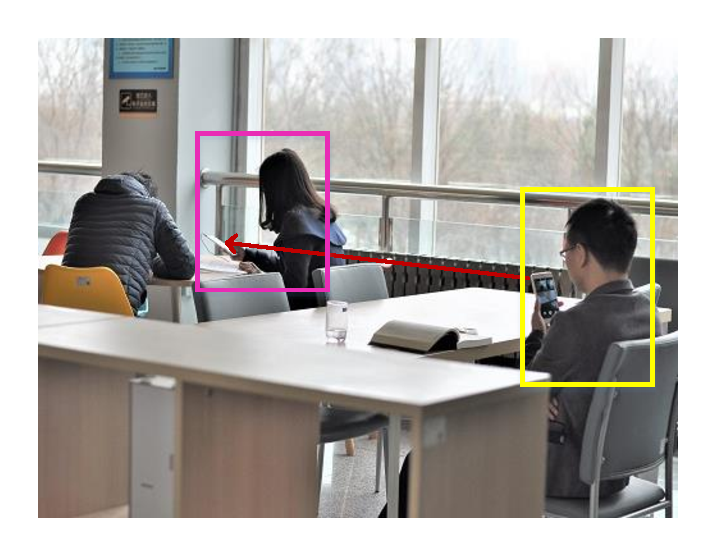
\includegraphics[height=3cm]{fig/1-1.pdf}\\
             \footnotesize (a) A common attacking scenario.
            \end{minipage}
        }
        \hspace{0.5cm}
        \subfigure{
            \begin{minipage}[t]{3.5cm}
            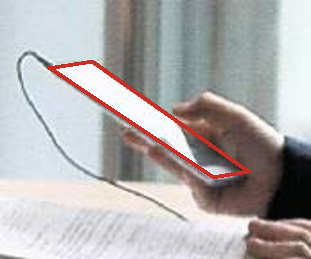
\includegraphics[height=3cm]{fig/1-2.pdf}\\
             \footnotesize (b) The device screen seen from the video filmed in (a).
            \end{minipage}
        }
        \subfigure{
            \begin{minipage}[t]{3.5cm}
            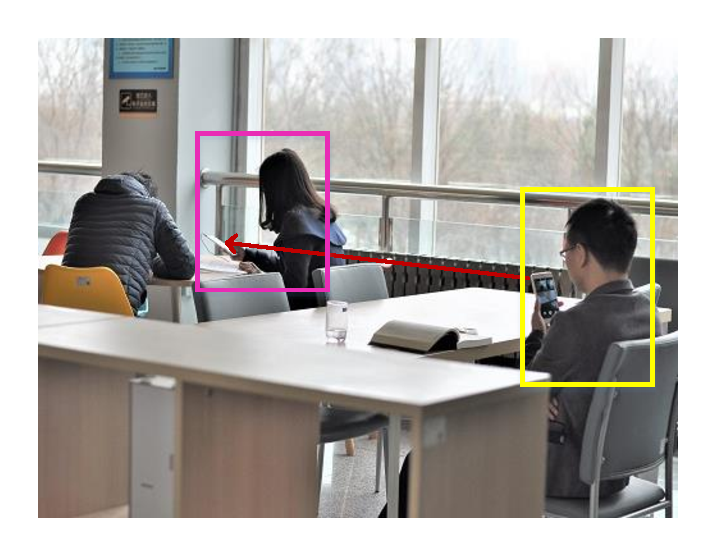
\includegraphics[height=3cm]{fig/1-3.pdf}\\
             \footnotesize (c) The video was recorded from a distance of 2.5 meters.
            \end{minipage}
        }
        \hspace{0.5cm}
        \subfigure{
            \begin{minipage}[t]{3.5cm}
            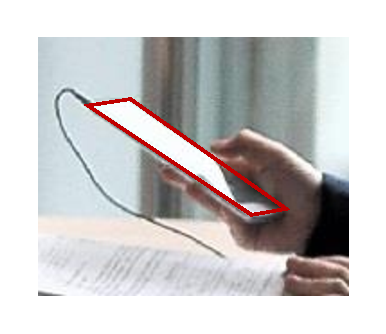
\includegraphics[height=3cm]{fig/1-4.pdf}\\
             \footnotesize (d) The device screen seen from the video filmed in (c).
            \end{minipage}
        }
        \subfigure{
            \begin{minipage}[t]{3.5cm}
            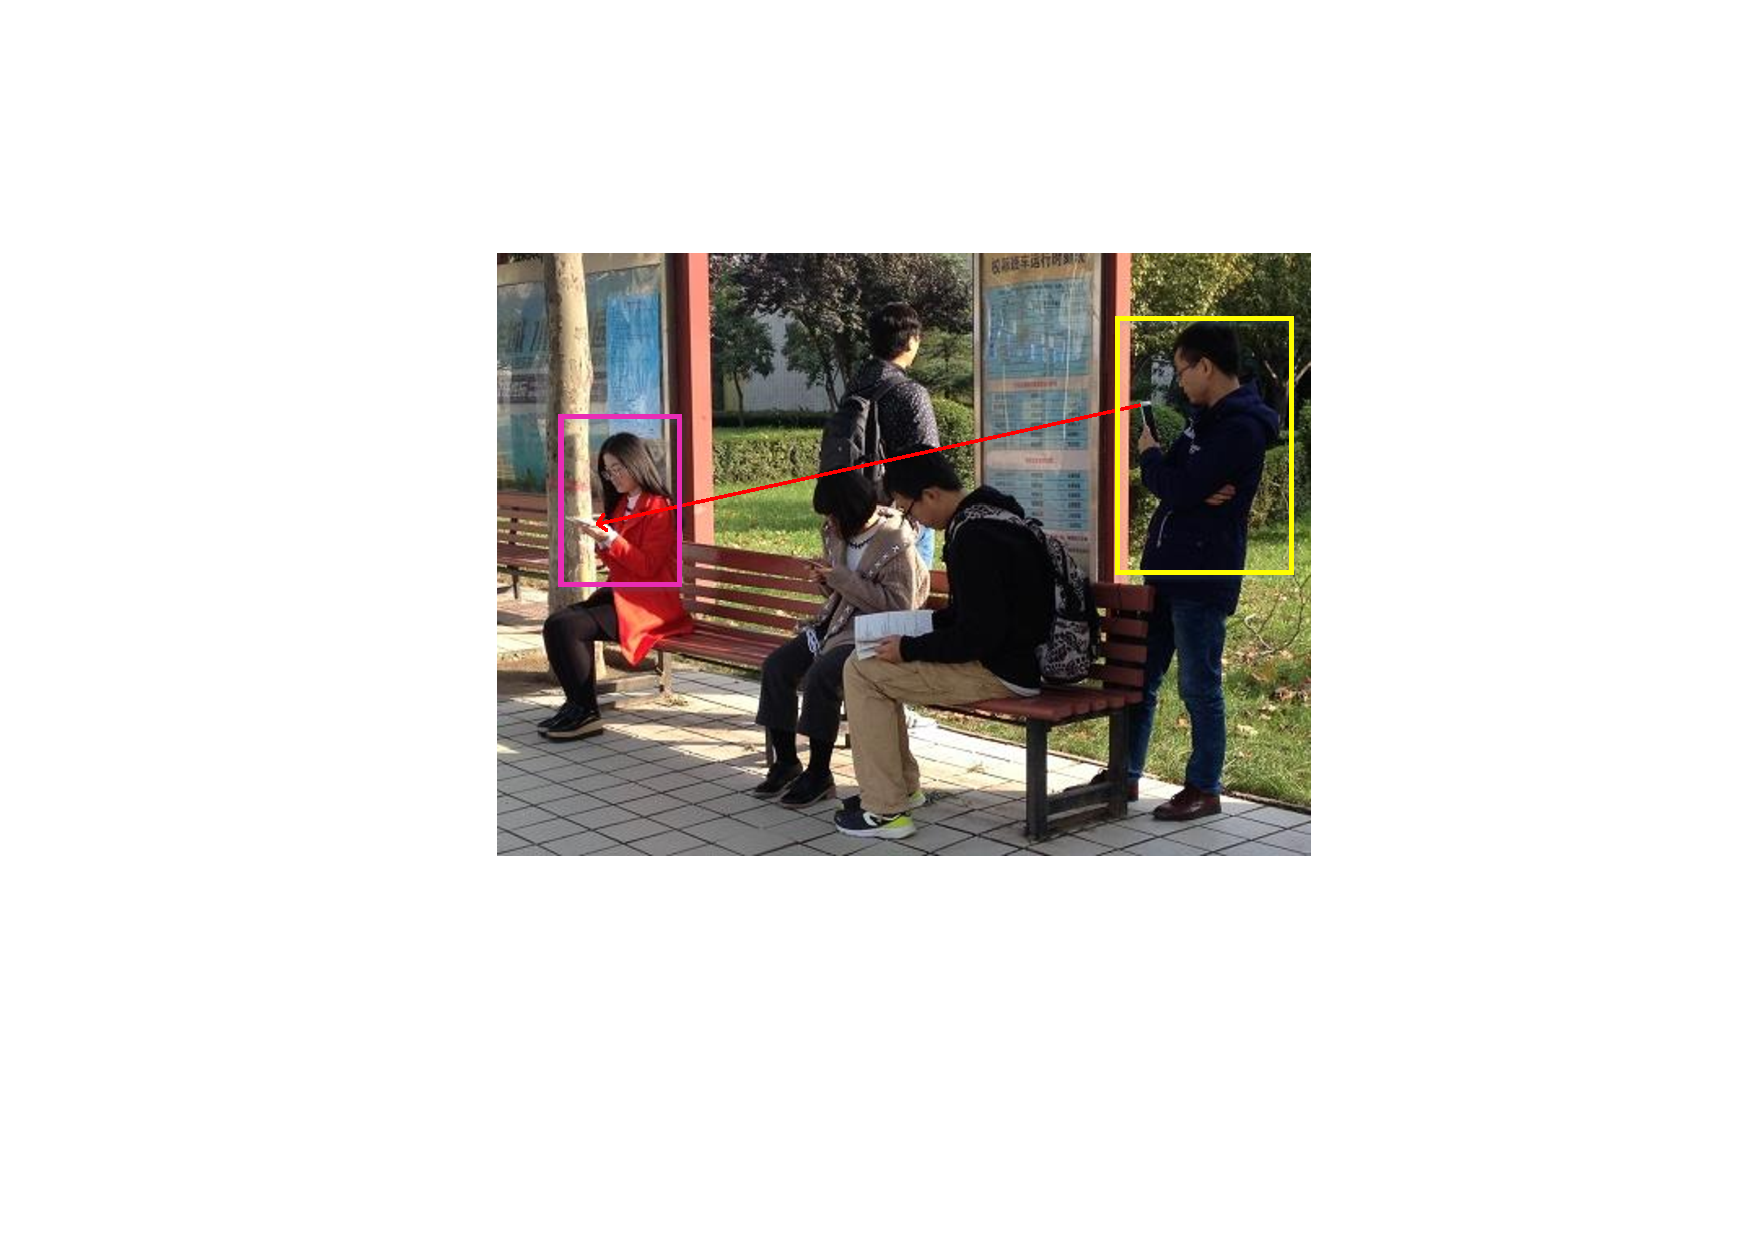
\includegraphics[height=3cm]{fig/1-5.pdf}\\
             \footnotesize (e) An outdoor scenario.
             %The user is focusing his attention on searching for learning material in classroom.
            \end{minipage}
        }
        \hspace{0.5cm}
        \subfigure{
            \begin{minipage}[t]{3.5cm}
            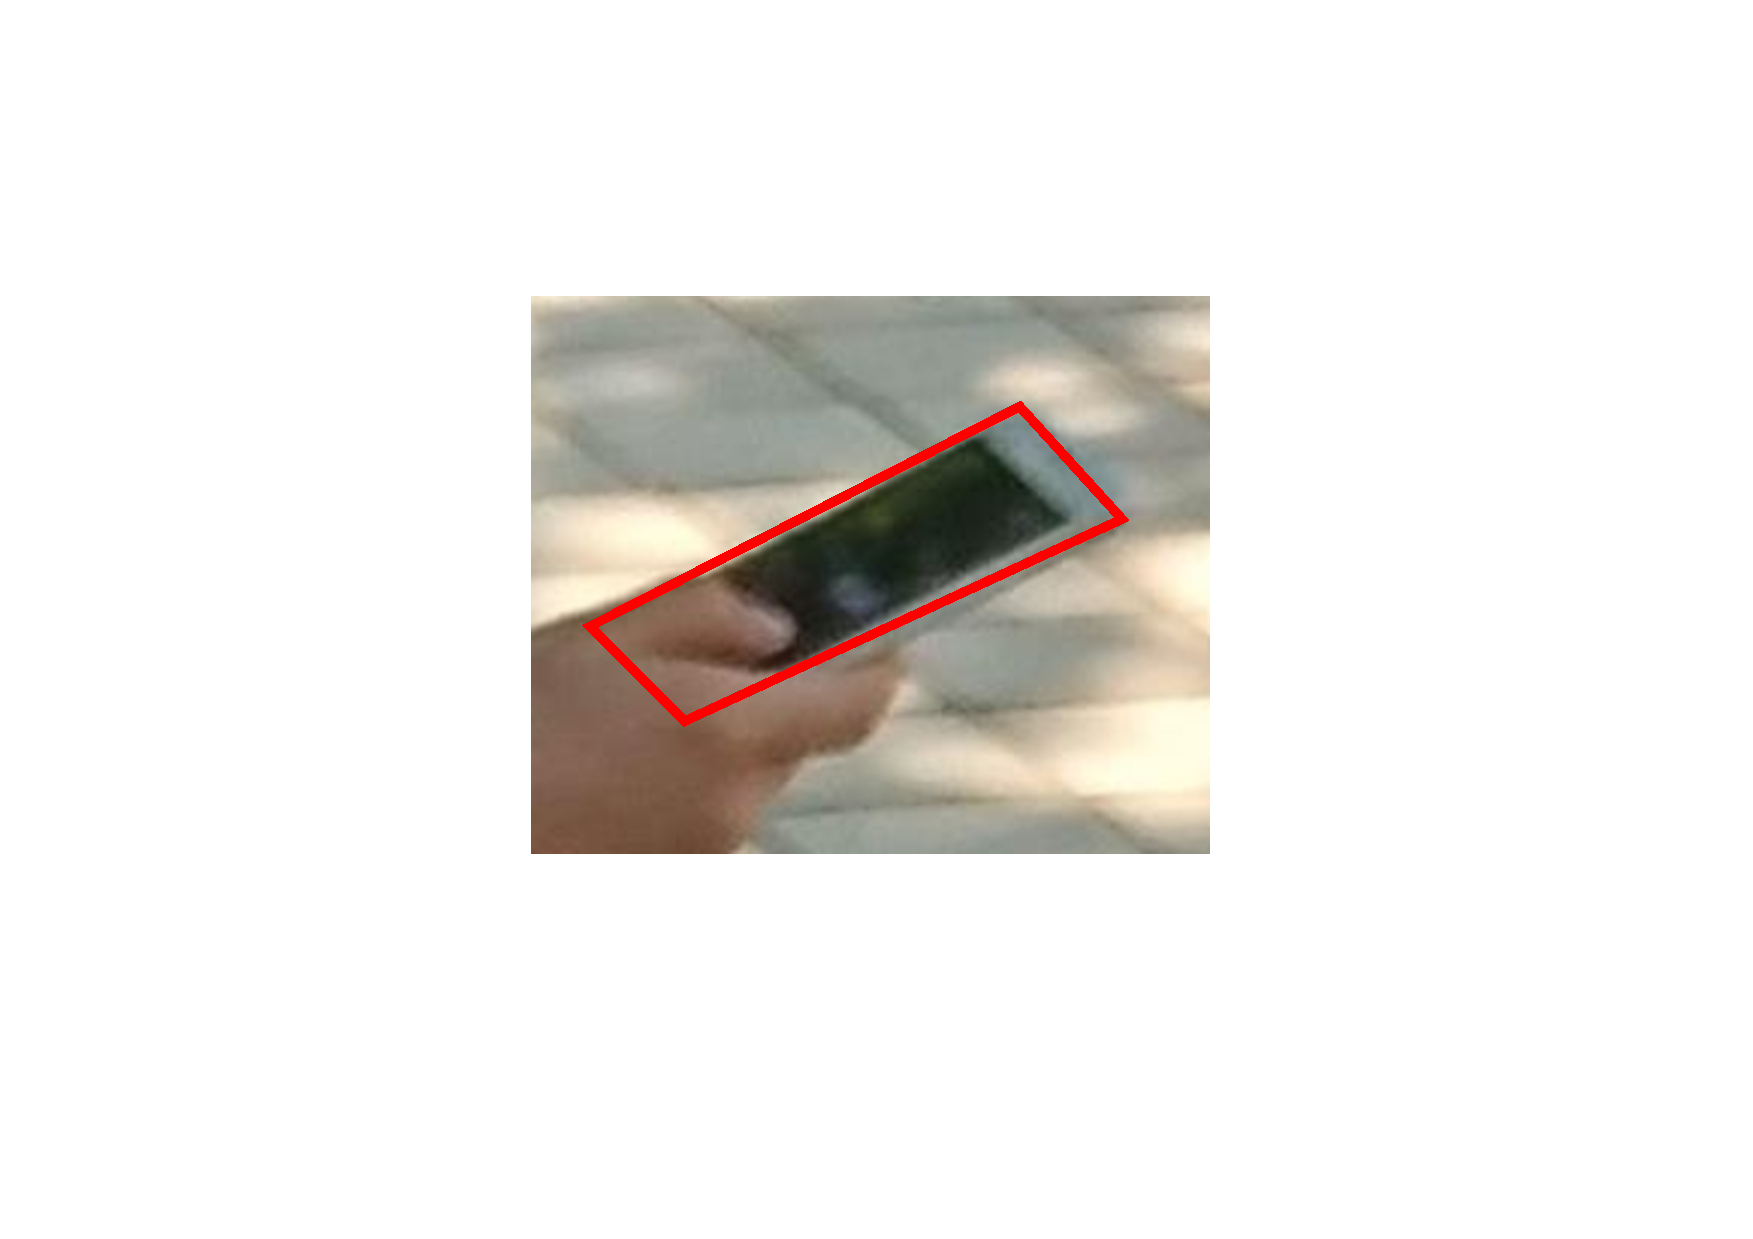
\includegraphics[height=3cm]{fig/1-6.pdf}\\
             \footnotesize (f)
             The device screen seen from the video filmed in (e).
            \end{minipage}
        }
        \caption{Examples of scenarios in which a mobile phone camera is used to film the unlocking process.
        In these scenarios, the camera does not need to have a clear sight of the screen.}
        \label{fig:fig1}
    \end{figure}


We thoroughly evaluate our approach using 120 unique patterns collected from independent users. We show that our approach is effective in inferring candidate patterns and as a result, an attacker can unlock
the target device with a success rate of over 95\% (up to 97.5\%) in five attempts.
We demonstrate that, in contrast to many people's belief, complex patterns do not provide stronger protection over simple patterns under our attack. According to a recent study~\cite{alpnorway}, people tend to use complex
patterns for critical applications such as online banking and shopping applications.
Our finding suggests that using pattern lock to protect sensitive information could be risky.
%\FIXED{Intuitively, our approach is able to crack PIN-based passwords by analyzing the fingertip movement when typing the passwords. We evaluate our approach using 30 four-digital PIN-based passwords and the experimental result shows we can break most of passwords within five attempts.}
%
%\FIXED{Given the wide usage of pattern lock, we propose a countermeasure to defend against video-based attack without external hardware. This method can effectively confuse the attack to infer correct pattern by disabling a necessary attack factor--user can draw any pattern before or after drawing the correct pattern.}

\vspace{3mm}
\noindent \textbf{Contributions} The key contribution of this paper is a new
attack for Android pattern lock. Our attack exploits techniques
developed in the computer vision domain to address the key
challenges highlighted above.


This paper makes the following specific contributions:


\begin{itemize}
\item \emph{A New Attack.}% This is the first work on exploiting video-based side-channels to attack
%Android pattern lock (Section~\ref{section:overview}).
This is the first work to reconstruct locking patterns without relying on
the content shown on the screen (Section~\ref{sec:scenarios}). %Our approach can accurately
%extract the correct pattern from video footage filmed using a mobile camera that does not directly faces the target device.
Experimental results show that our method can break over
95\% of the lock patterns in five attempts (Section~\ref{sec:overall_rate}). Given that the Android
operating system (OS) allows five tries before
locking the device, our attack represents a real threat for pattern lock.

\item \emph{Identifying New Vulnerabilities.} According to a recent study~\cite{DBLP:conf/soups/2014}, direct
observation techniques, e.g. shoulder surfing, are considered to be a low risk due to the close distance between the
attacker and the user (in order to gain a clear sight of the device screen). As a result, many users may underestimate
the risks of using pattern lock in public places. Under our attack, filming can be carried out at a distance of 2
meters from the user and the camera does not need to directly face the target device. Such a camera setting makes our
attack less likely to raise suspicion, but rather more likely to success when compared to direct observation
techniques. For instance, the video can be filmed by an adversary who pretends to interact with his phone, sitting next
to the user in a public place (see Figure~\ref{fig:fig1}). In many similar scenarios, many users will not be suspicious
of the attacker's behavior.

\item \emph{New Findings.} Our study suggests that complex patterns are more vulnerable
under video-based attacks (Section~\ref{sec:overall_rate}). This finding debunks many people's conception
that more complex patterns give stronger protection. Therefore, our work sheds new insights on
 the practical use of pattern lock. We also show that by making some small modifications to the
 pattern lock can significantly reduce the risk of the presented attack.

\end{itemize}

\begin{figure*}[!ht]
    \centering
    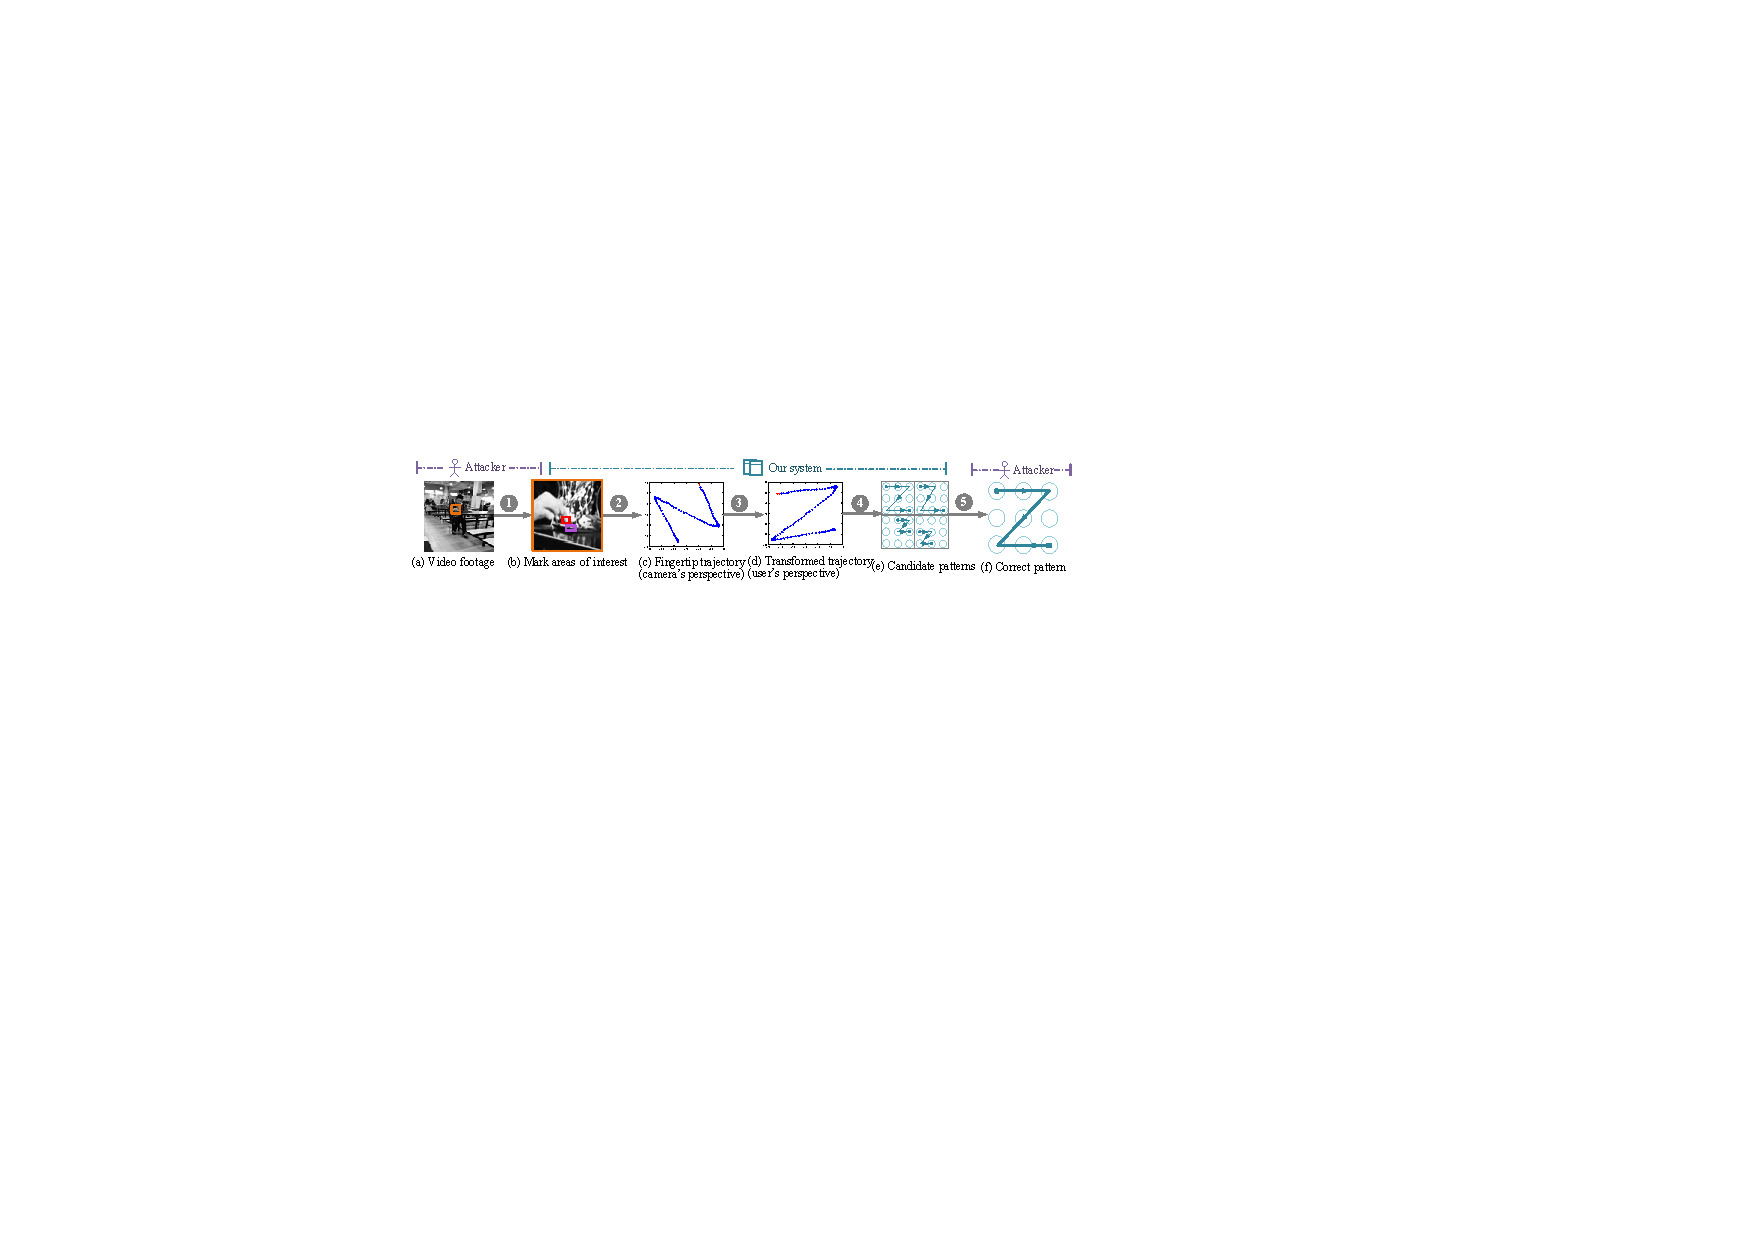
\includegraphics[width=\textwidth]{fig/overview.pdf}
    \vspace{-4mm}
    \caption{Overview of the attack.
     Our system takes in a video segment that records the unlocking process (a). The adversary first marks two areas of interest on the first video frame (b): one contains the fingertip involved in pattern drawing, and the other contains part of the device. Our system then tries to track the fingertip's location w.r.t. to the device.
     The tracking algorithm produces a fingertip movement trajectory from the camera's perspective (c) which is then transformed to the user's perspective (d). Finally, the resulted trajectory in (d) is mapped to several candidate patterns (e) to be tested on the target device (f). }
    \label{fig:fig2}
    \vspace{-3mm}
\end{figure*}

\section{Background}
    \subsection{Android Pattern Lock}
    \label{section: android_pattern_lock}
        Pattern lock is widely used to protect sensitive information and perform authentication on
        Android touch-screen devices. \FIXED{The motivation for user to prefer to pattern lock is that graphical passwords are easily to be recalled comparing to alphanumeric characters~\cite{standing1970perception,Weiss2008PassShapes}.}
        To unlock a device protected with pattern lock, the user is asked to draw a predefined sequence of connected dots on a pattern grid\footnote{In this paper we use the Android default pattern grid with $3 \times 3$ dots, unless otherwise stated.}.
        Figure~\ref{fig:fig2} (e) shows a pattern which consists of seven dots on a $3 \times 3$ grid.
        To form a
        pattern, the user starts by selecting one dot as the
        starting point and then swiping over multiple dots of the grid until the fingertip is lifted from the screen.
        %Essentially, pattern lock is a simplified variant of
%        the Pass-Go graphical based password scheme
%        \cite{biddle2012graphical}.
        There are several rules for creating an Android pattern: (1) a pattern must consist
        of at least four dots; (2) each dot can only be visited once; and (3) a previously unvisited dot will
        become visited if it is part of a horizontal, vertical or diagonal
        line segment of the pattern. Taking into account these constraints, the total number of possible patterns
        on a $3\times3$ grid is 389,112~\cite{uellenbeck2013quantifying}.
        Given the large number of possible patterns, performing brute-force attacks on
        Android pattern lock is ineffective, because the device will be
        automatically locked after five failed tries.
        \FIXED{Further, the brute-force attack is hard to guess those patterns with complex structures comparing to text-based passwords~\cite{Kelley2012Guess,Mazurek2013Measuring}.}

    \subsection{Threat Model}
    \label{sec:scenarios}
        In our threat model, we assume an adversary wants to access some sensitive information from or to install malware on a
target device that is protected by pattern lock. This type of attacks is mostly likely to be performed by an attacker
who can physically access to the target device for a short period of time (e.g. via  attending a meeting or a party where
the user presents). To quickly gain access to the device, the attacker would like to obtain
the user's locking pattern in advance.

The attack starts from filming how the user unlocks the device. Video recording
can be done on-site or ahead of time. The video will then be processed to identify a small number of patterns to be
tested on the target device. Because filming can be carried out from a distance of as far as 2 meters using a
mobile phone camera and the camera does not need to directly face the target device, this activity often will not be
noticed by the user. Moreover, given that many users use the same pattern across devices and applications, the pattern
obtained from one device could also be used to break the user's other devices.  We want to stress that the goal of this paper is to
demonstrate the feasibility of a new attack and the countermeasure is left to our future work.

\vspace{2mm}
\noindent \textbf{Examples of Filming Scenarios} Figure~\ref{fig:fig1} illustrates three scenarios where filming can be
performed without raising suspicion to many users. For all the examples presented in Figure~\ref{fig:fig1}, the
filming camera had a left- or right-front view angle from the target device and did not directly face the screen of the target device. Due to the filming distance (2-3 meters), the recoded video typically does not have a clear vision of
the content displayed on the screen.  This observation can be confirmed by the video snapshot placing
alongside each scenario, where it is impossible to identify the content shown on the screen.
The examples given in Figure~\ref{fig:fig1} are some of the day-to-day
scenarios where security of the user's device can be compromised under
our attack.

\vspace{2mm}
\noindent \textbf{Assumptions}
Our attack requires the video footage to have a vision of the user's
fingertip that was involved in pattern drawing as well as part of the device (e.g. an edge of a phone).
We believe this is a reasonable assumption because in practice many users often do not fully cover their fingers and the entire device when drawing a pattern.
This is particularly true when holding a large-screen device by hands.
To launch the
attack, the attacker needs to know the layout of the grid, e.g. whether it is
a $3 \times 3$ or a $6 \times 6$ grid. Our approach is to generate a set of
candidate patterns for each of the Android pattern grids and the attacker can simply decide
which set of candidate patterns to use after seeing the target device (at the time the
layout of the grid will be available). However, unlike prior work on
video-based attacks on keystroke based authentication~\cite{shukla2014beware}, our approach does not
require having knowledge of the console's geometry. In other words, the size
of the screen or the position of the pattern grid  on the screen does not
affect the accuracy of our attack. We also assume the video does not need to
capture any content displayed on the screen. This assumption makes previous
video-based attacks on pattern lock~\cite{aviv2010smudge} inapplicable.

\section{Overview of The Attack}
\label{section:overview}
    In this section, we give an overview of our attacking system which analyzes the user's fingertip movement to infer the locking pattern. The system takes in a video segment that records the entire unlocking process. It produces a small number of candidate patterns to be tested on the target device.
    Figure~\ref{fig:fig2} depicts the five steps of our attack:

    %\begin{enumerate}
    \vspace{2mm}
    \noindent \circled{1} \textbf{Filming and Video Preprocessing:} The attack begins from
        filming how the pattern is drawn. The video footage can be filmed at a distance of
        about 2 meters from the user using a mobile phone camera (or 9 meters using a digital single reflex camera). After recording, the attacker
        needs to cut out a video segment that contains the entire unlocking
        process. We have shown that it is possible to automatically identify this video segments in some scenarios (Section~\ref{sec:identify}).
        After cutting out the video segment, the attacker is then asked to mark two areas of interest from a video frame: one area consists of
        the fingertip used to draw the pattern, and the other consists of part of the device (see
    Figure~\ref{fig:fig2} (b)).

     \vspace{2mm}
    \noindent \circled{2}  \textbf{Track Fingertip Locations:} Once the areas of interest are highlighted, a computer vision algorithm will be applied
        to locate the fingertip from each video frame (Section~\ref{secction:shake}). The algorithm aggregates the successfully tracked fingertip locations to produce a fingertip movement trajectory.
        This is illustrated in Figure~\ref{fig:fig2} (c). Keep in mind that at this stage the tracked trajectory is presented from the camera's perspective.

     \vspace{2mm}
    \noindent \circled{3} \textbf{Filming Angle Transformation:}  This step transforms the tracked fingertip locations from the camera's perspective to the user's.
    We use an edge detection algorithm to automatically calculate the filming angle which is then used to perform the transformation (Section~\ref{sec:transformation}).
    For example, Figure~\ref{fig:fig2} (c) will be transformed to Figure~\ref{fig:fig2} (d) to obtain a fingertip movement trajectory from the user's perspective.

     \vspace{2mm}
    \noindent \circled{4} \textbf{Identify and Rank Candidate Patterns:} In this step, our software automatically maps the tracked fingertip movement trajectory to a number of candidate patterns (Section~\ref{section:spea}).
    We rank the candidate patterns based on a heuristic described in Section~\ref{section:identity}.
    For instance, the fingertip movement trajectory in Figure~\ref{fig:fig2} (d) could be mapped to a number of candidate patterns shown in Figure~\ref{fig:fig3}.
    Our approach is able to reject most patterns to leave no more than five candidate patterns to be tried out on the target device.

     \vspace{2mm}
    \noindent \circled{5} \textbf{Test Candidate Patterns:} In this final step, the attacker tests the candidate patterns on the target device.



\begin{figure}[!t]
    \centering
    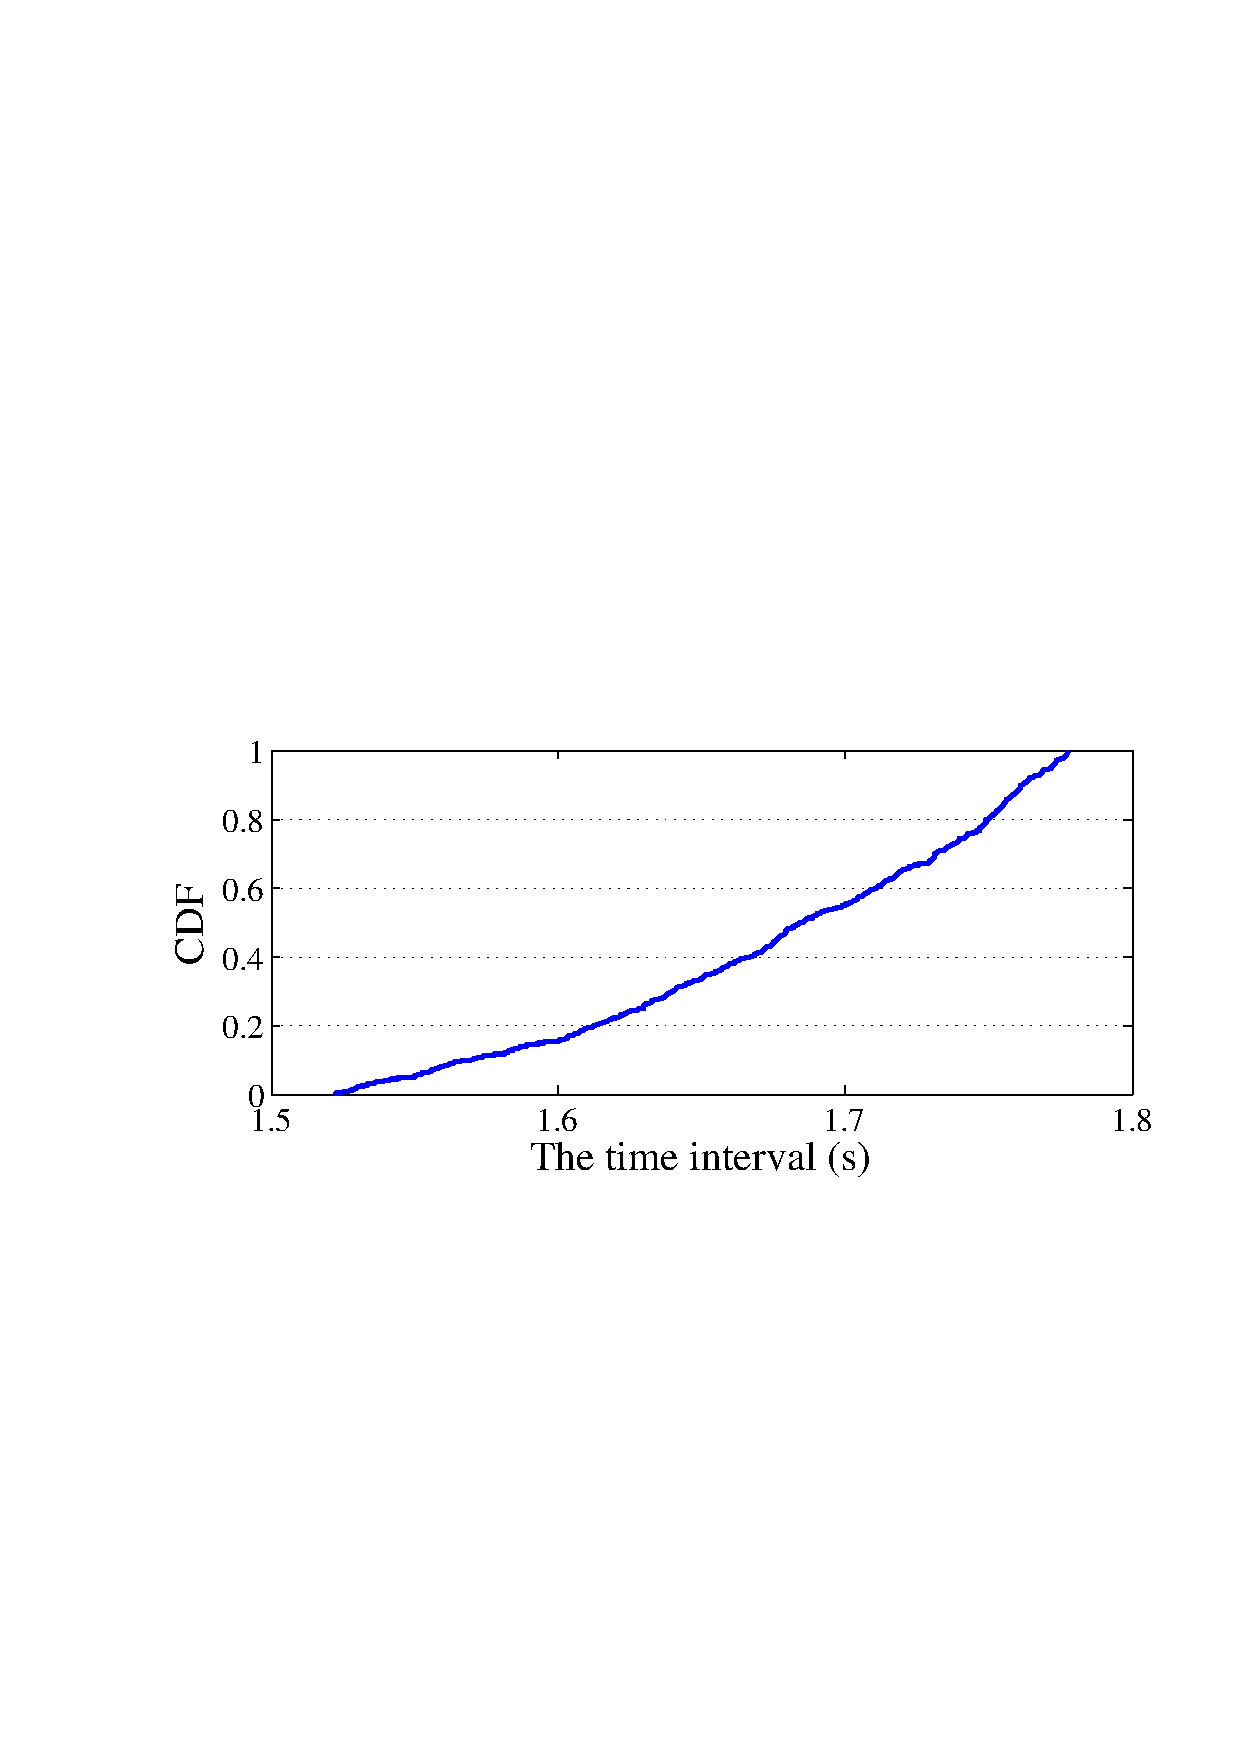
\includegraphics[width=0.45\textwidth]{fig/time-interval.pdf}
    \caption{The cumulative distribution function (CDF) of the time interval between pattern drawing and other on-screen activities.}
    \label{fig:time-interval}
\end{figure}

    \begin{figure}[!t]
        \centering
        \subfigure{
            \begin{minipage}[t]{0.19\textwidth}
            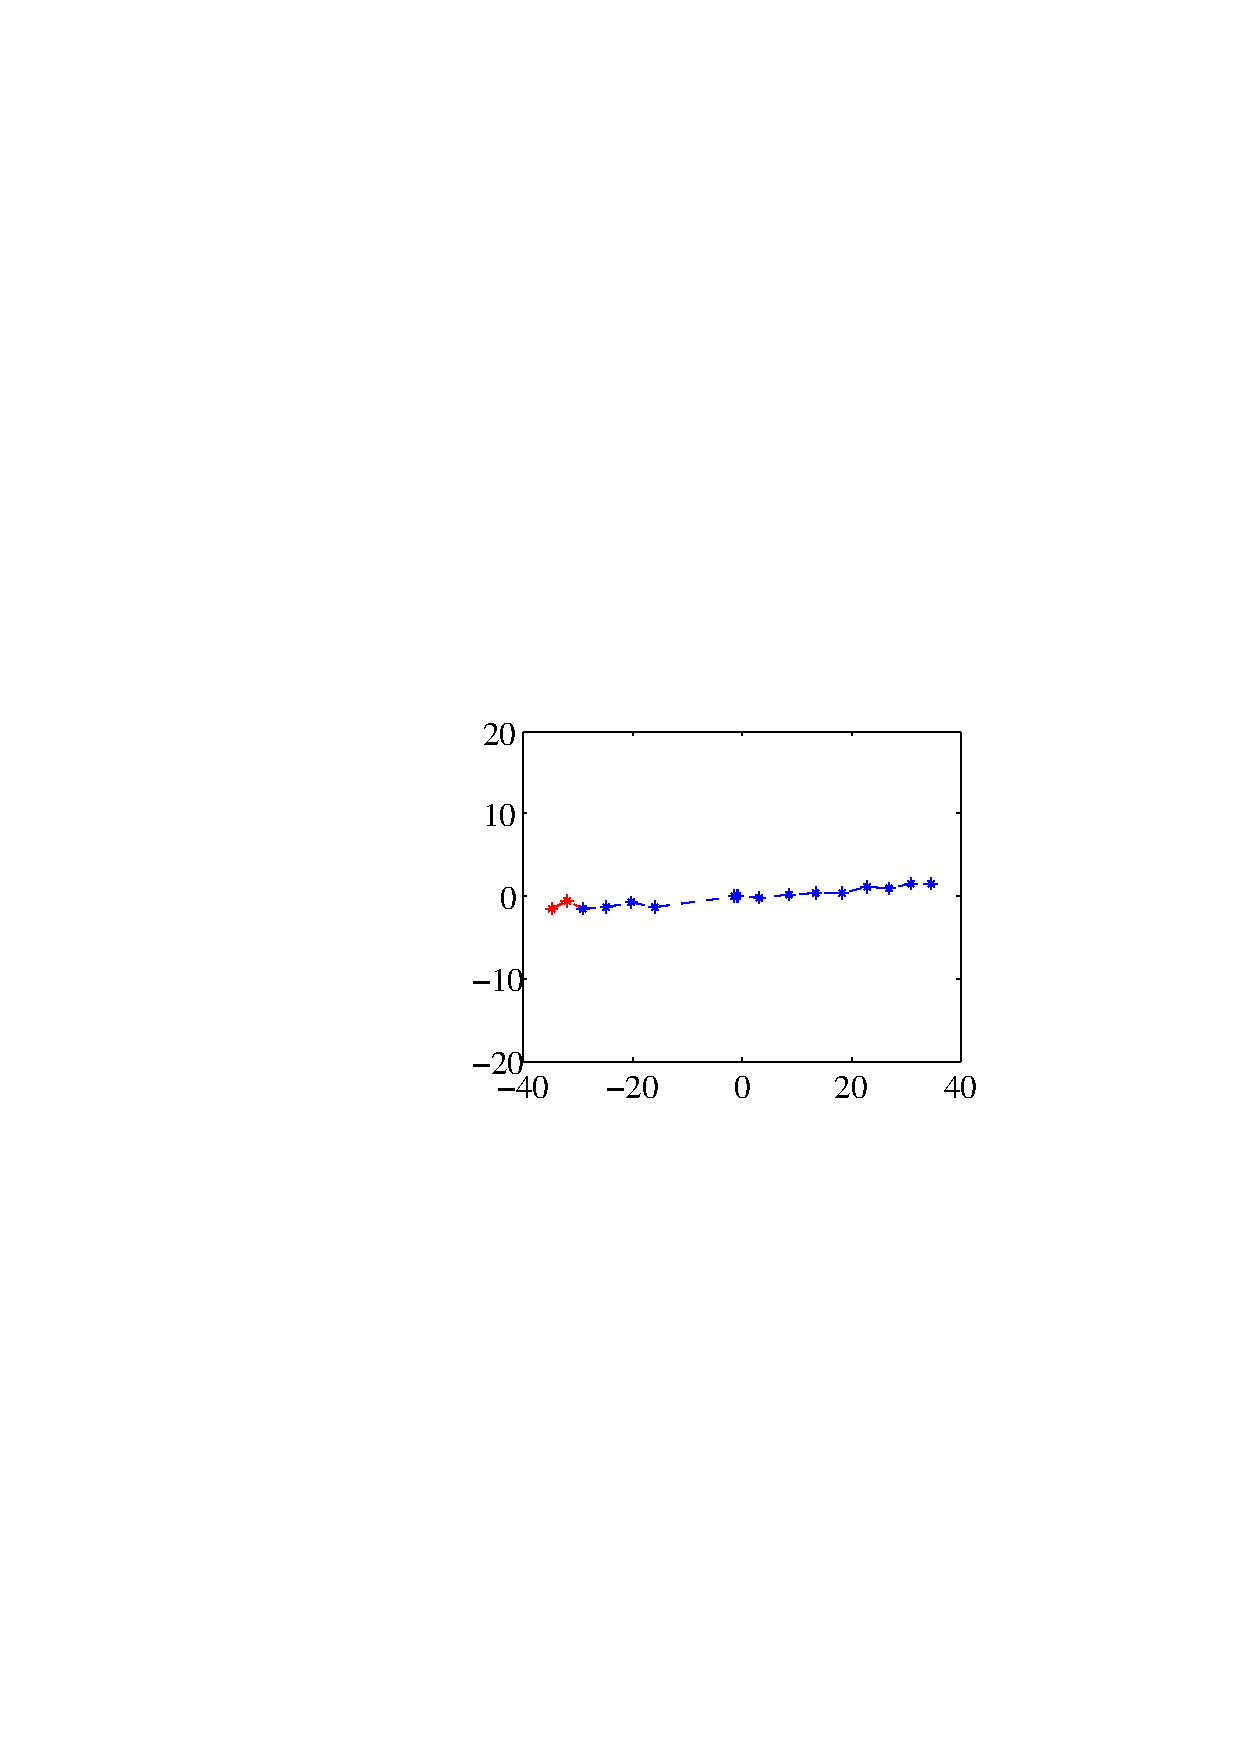
\includegraphics[width=\textwidth]{fig/gesture-distinction1.pdf}\\
            \centering  (a) a horizontal-swiping gesture
            %\FIXME{Need to mark the starting point and turning point}
            \end{minipage}
        }
        \hspace{0.25cm}
        %\hfill
        \subfigure{
            \begin{minipage}[t]{0.19\textwidth}
            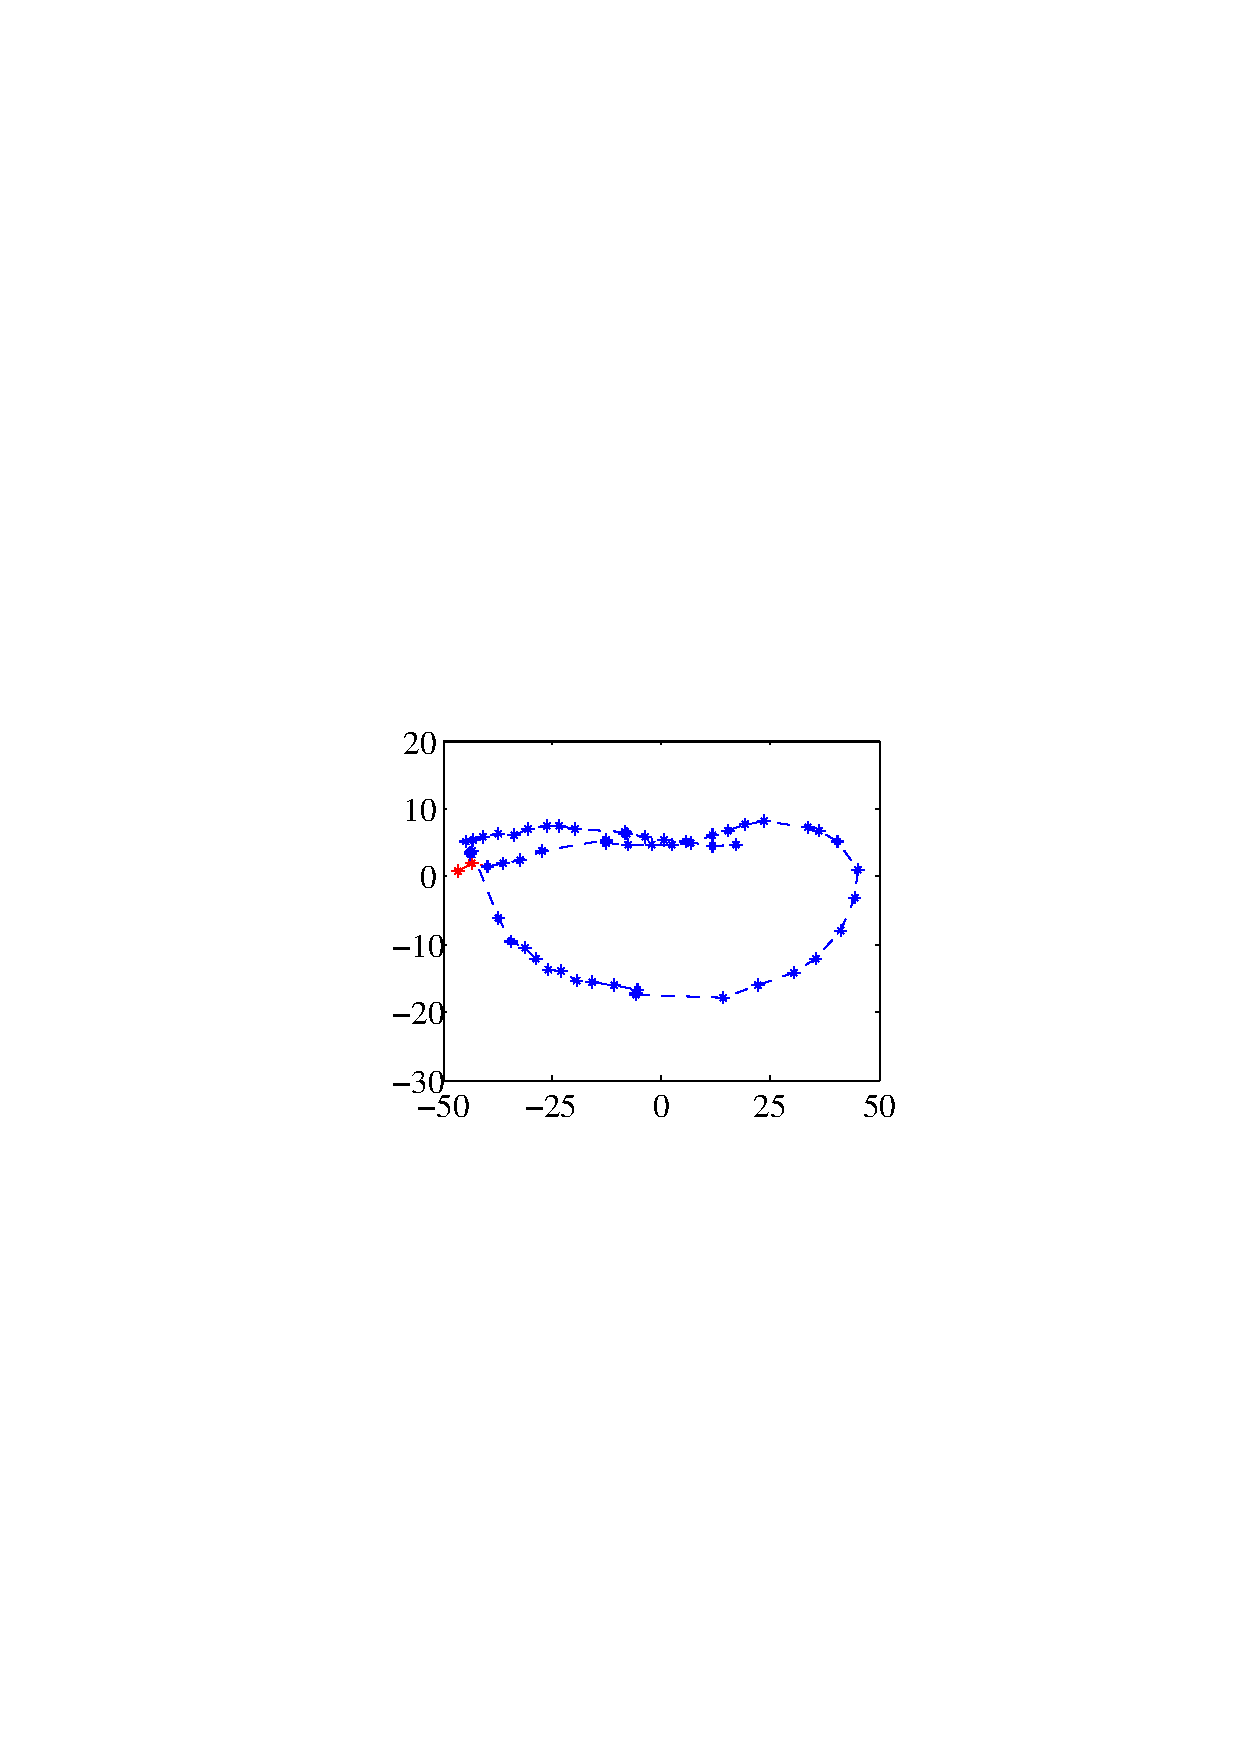
\includegraphics[width=\textwidth]{fig/gesture-distinction2.pdf}\\
            \centering  (b) two consecutively horizontal-swiping gestures
            \end{minipage}
        }
        \subfigure{
            \begin{minipage}[t]{0.19\textwidth}
            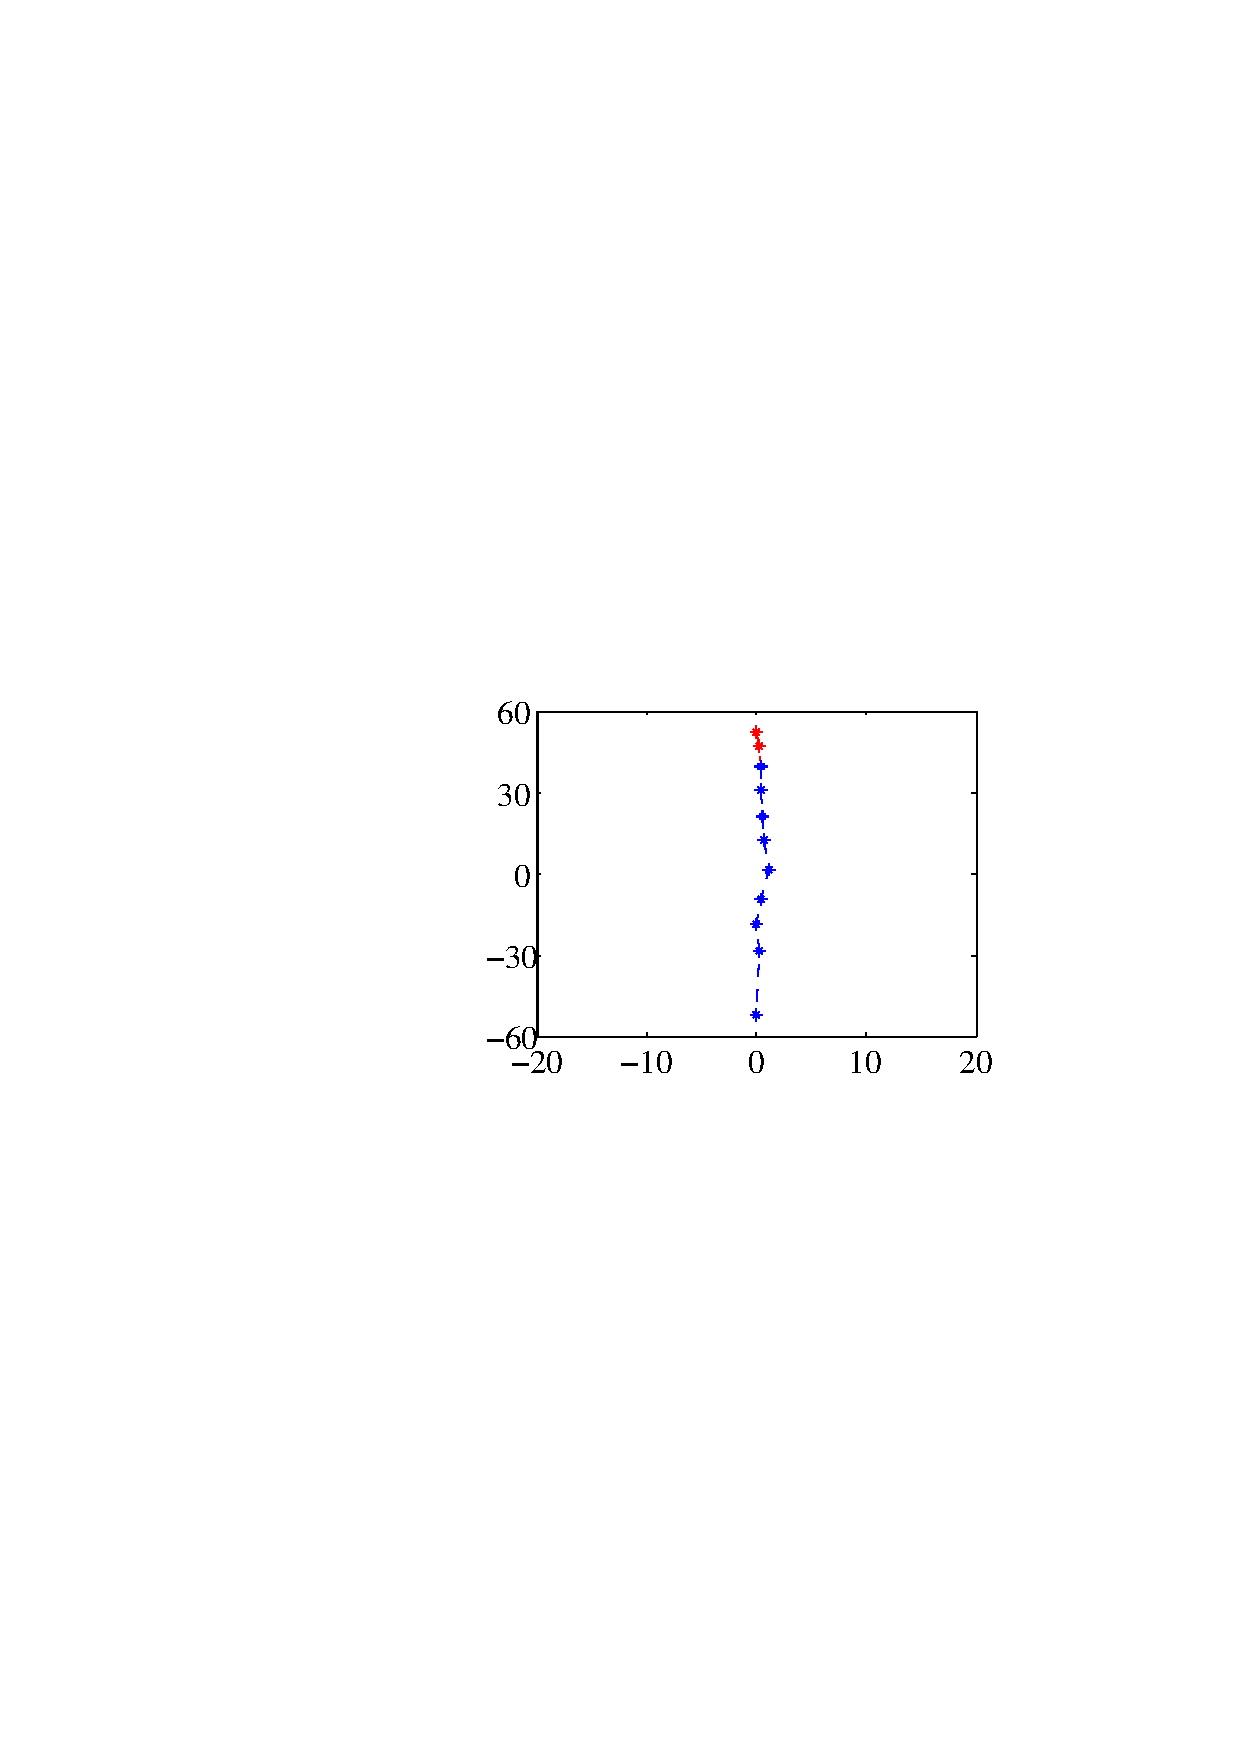
\includegraphics[width=\textwidth]{fig/gesture-distinction3.pdf}\\
            \centering  (c) a vertical-swiping gesture
            %\FIXME{Need to mark the starting point and turning point}
            \end{minipage}
        }
        \hspace{0.25cm}
        %\hfill
        \subfigure{
            \begin{minipage}[t]{0.19\textwidth}
            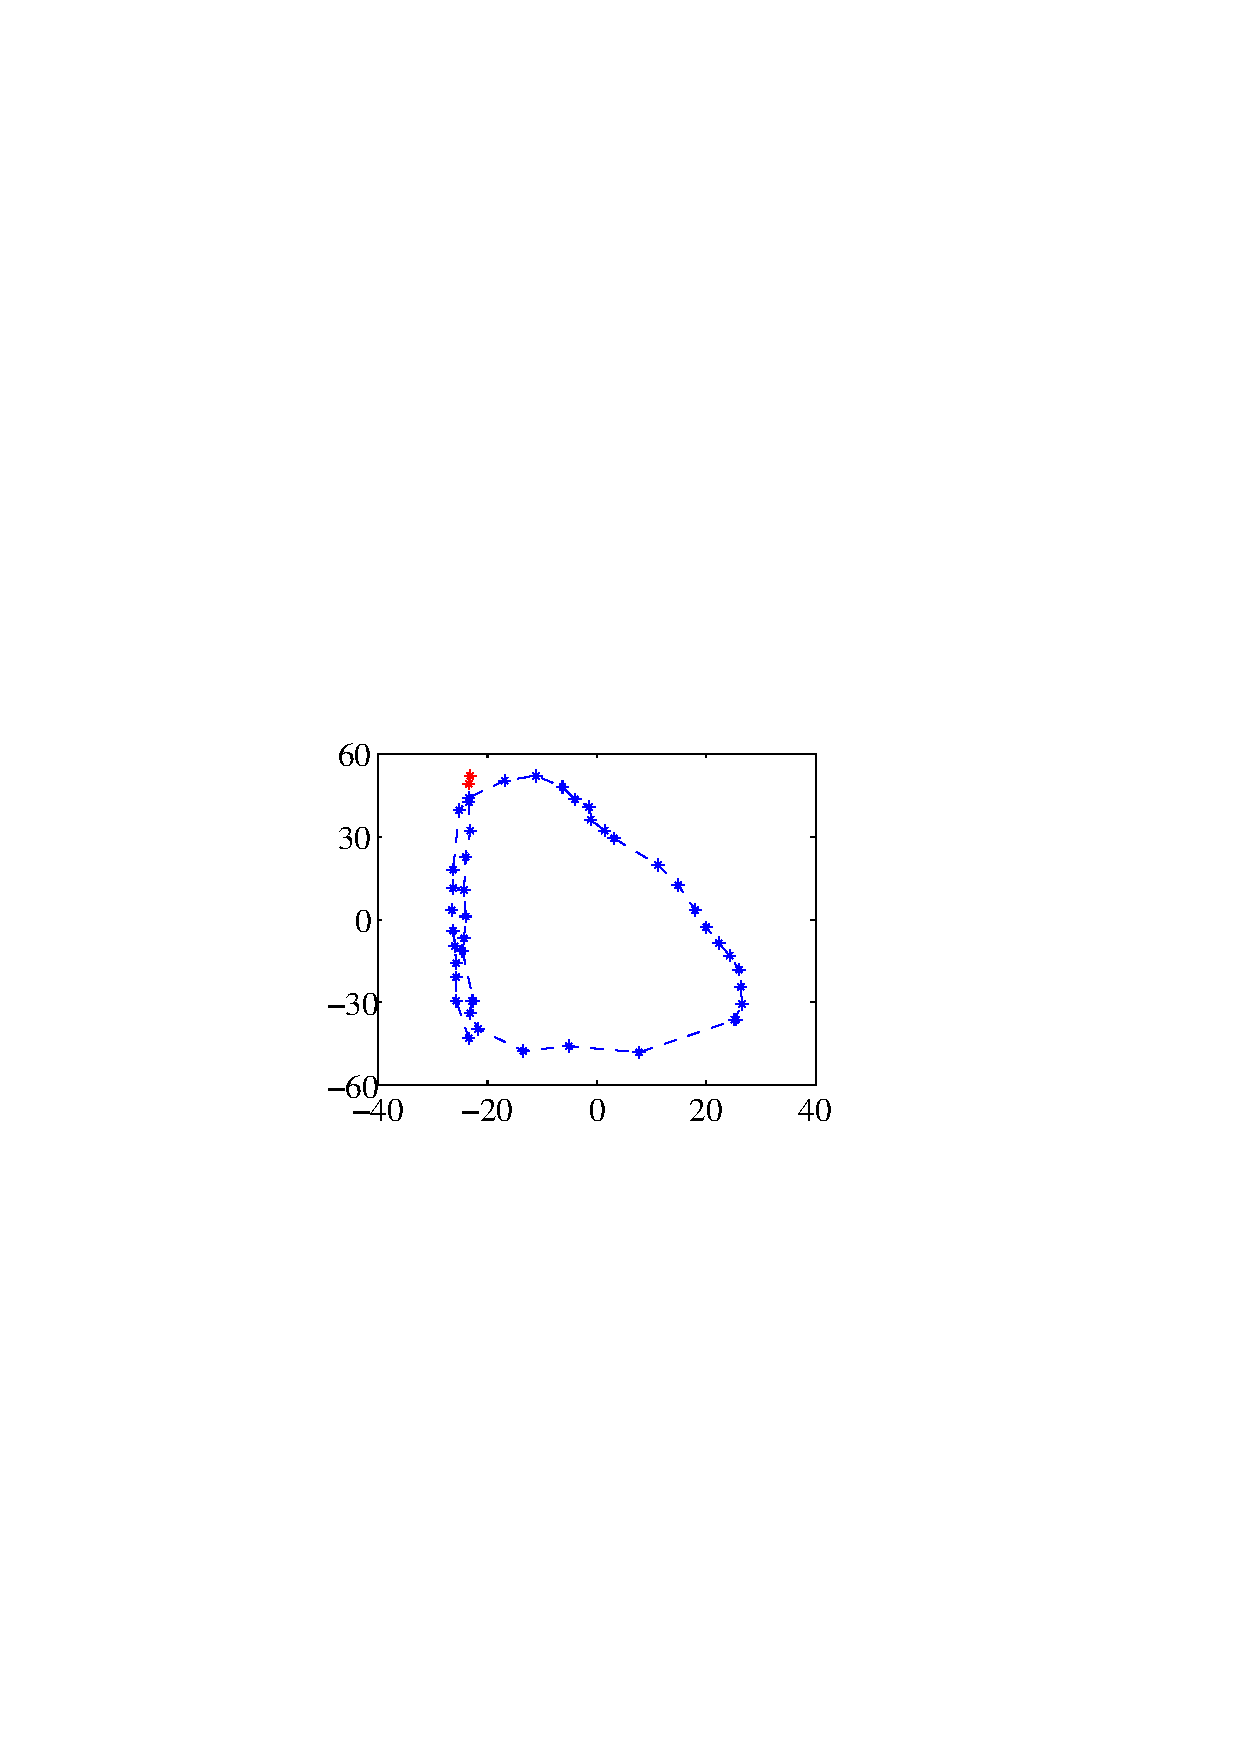
\includegraphics[width=\textwidth]{fig/gesture-distinction4.pdf}\\
            \centering  (d) two consecutively vertical-swiping gestures
            \end{minipage}
        }
        \subfigure{
            \begin{minipage}[t]{0.19\textwidth}
            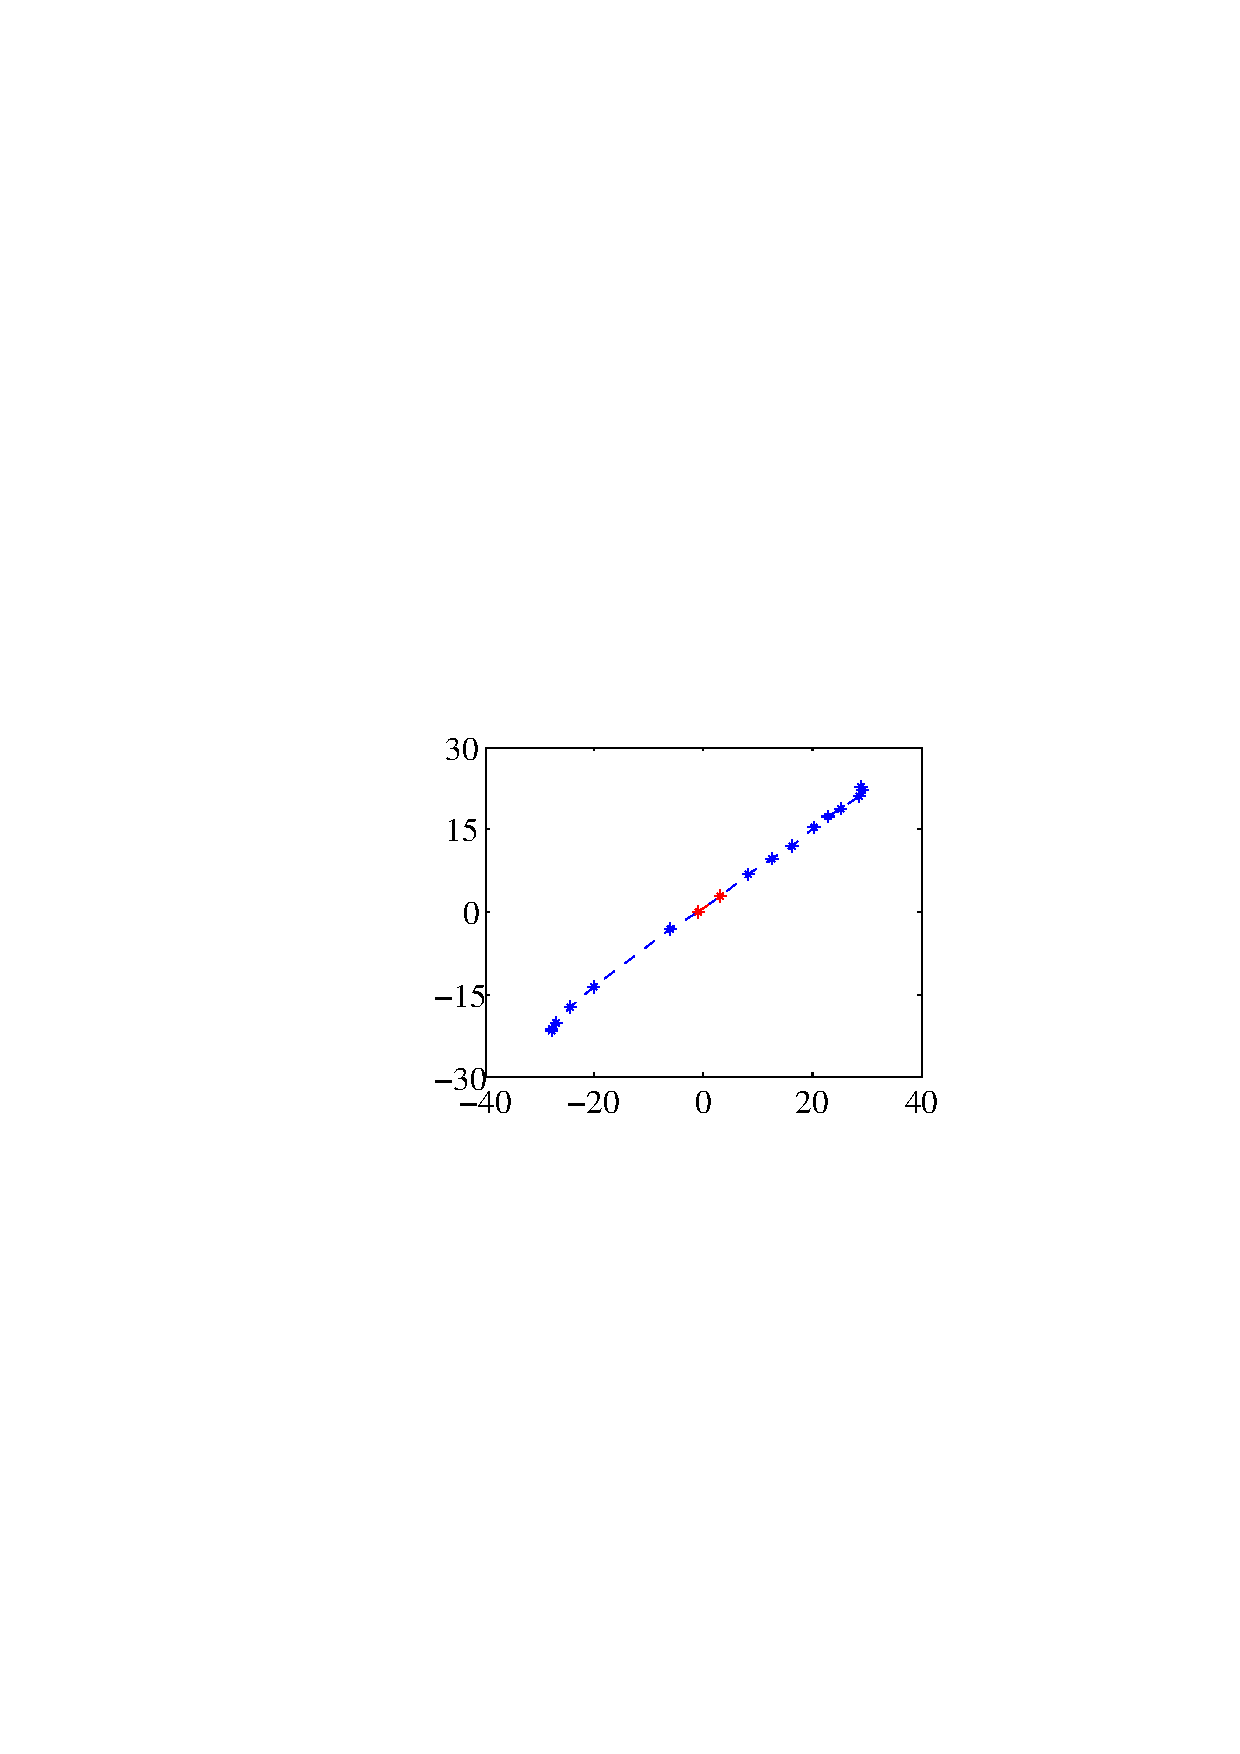
\includegraphics[width=\textwidth]{fig/gesture-distinction5.pdf}\\
            \centering  (e) a zooming gesture
            \end{minipage}
        }
        \hspace{0.25cm}
        %\hfill
        \subfigure{
            \begin{minipage}[t]{0.19\textwidth}
            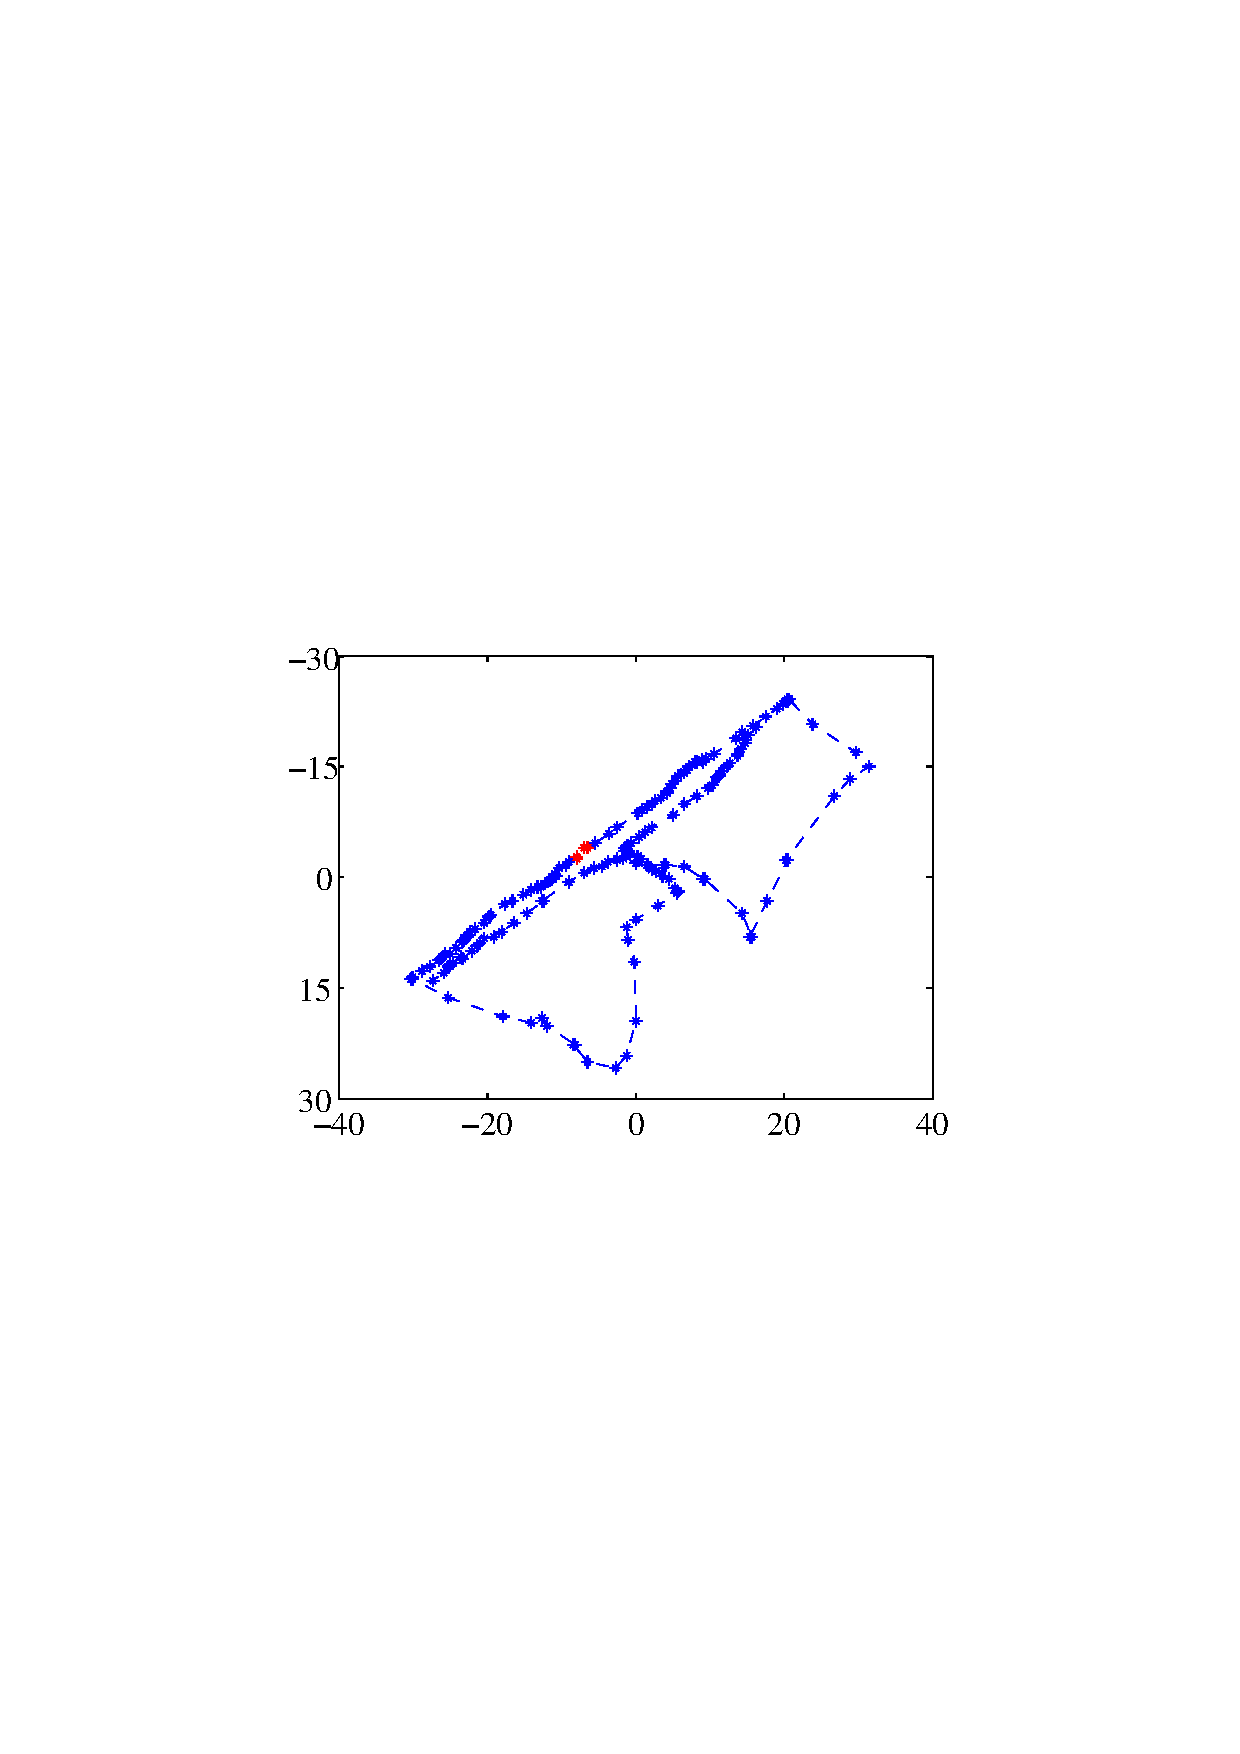
\includegraphics[width=\textwidth]{fig/gesture-distinction6.pdf}\\
            \centering  (f)two consecutive zooming gestures
            \end{minipage}
        }
        \caption{Spatial-temporal characteristics for performing an on-screen gesture once (a, c, e) and twice (b, d, f).}
        \label{fig:gesture-distinction}
    \end{figure}

    \begin{algorithm}[!t]
        \centering
        \caption{Unlocking process identification heuristic}
        %\FIXME{What is the threshold for fingertip location changes?}
        \label{alg:recognition}
        \begin{algorithmic}[1]
            \REQUIRE~~\\
                $IV$: Video footage  \\
                $frameCount$: Pause threshold before or after unlocking\\
                %$locationTh$: Threshold of fingertip location changes\\
            \ENSURE~~\\
                %$P[]$: Candidate patterns \\
                $<$start,end$>$: Start and end of the unlocking video segment \\
            \STATE $frames[] \leftarrow getVideoFrames(IV)$ \\
            \STATE $LEN \leftarrow getFramesLen(frames[])$ \\
            \FOR{$i=1:LEN-frameCount$}
                \STATE $sL \leftarrow hasFingertipChanged(frames[i:i+frameCount])$ \\
                \IF{$!sL$}
                    \STATE $sNo=i+frameCount$ \\
                    \FOR{$j=sNo:LEN$}
                        \IF{$checkLoop(frames[j:LEN])$}
                            \STATE $eNo=i$ \\
                            \STATE break; \\
                        \ELSIF{$!hasFingertipChanged(frames[j:j+frameCount])$}
                            \STATE $eNo=i$ \\
                            \STATE break; \\
                        \ENDIF
                    \ENDFOR
                    \STATE break;
                \ENDIF
            \ENDFOR
            \STATE $<start, end> \leftarrow getTargetVideo(frames[],sNo,eNo)$
        \end{algorithmic}
    \end{algorithm}

        \begin{figure*}[!t]
            \centering
            \subfigure{
                \begin{minipage}[t]{0.23\textwidth}
                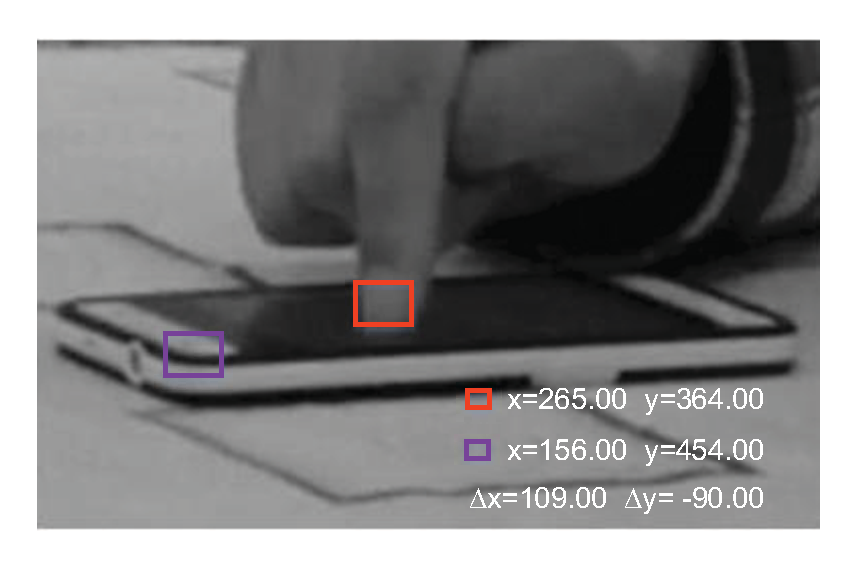
\includegraphics[width=1\textwidth]{fig/6--1.pdf}\\
                \centering  (a) The first video frame
                \end{minipage}
            }
            \hfill
            \subfigure{
                \begin{minipage}[t]{0.23\textwidth}
                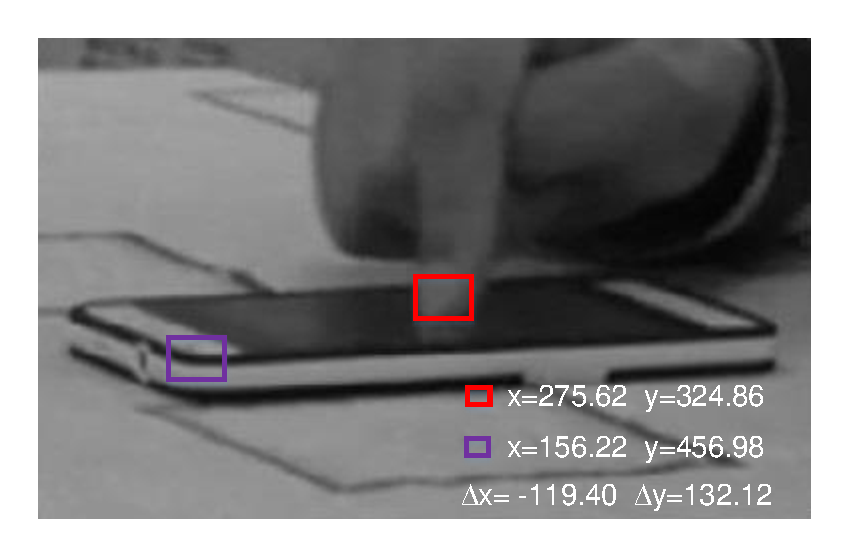
\includegraphics[width=1\textwidth]{fig/6--2.pdf}\\
                \centering  (b) A middle video frame
                \end{minipage}
            }
            \hfill
            \subfigure{
                \begin{minipage}[t]{0.23\textwidth}
                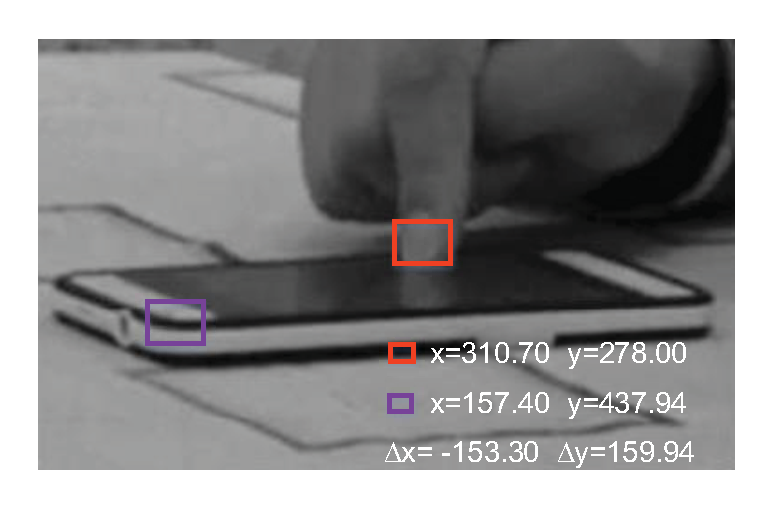
\includegraphics[width=1\textwidth]{fig/6--3.pdf}\\
                \centering  (c) The last video frame
                \end{minipage}
            }
            \hfill
            \subfigure{
                \begin{minipage}[t]{0.22\textwidth}
                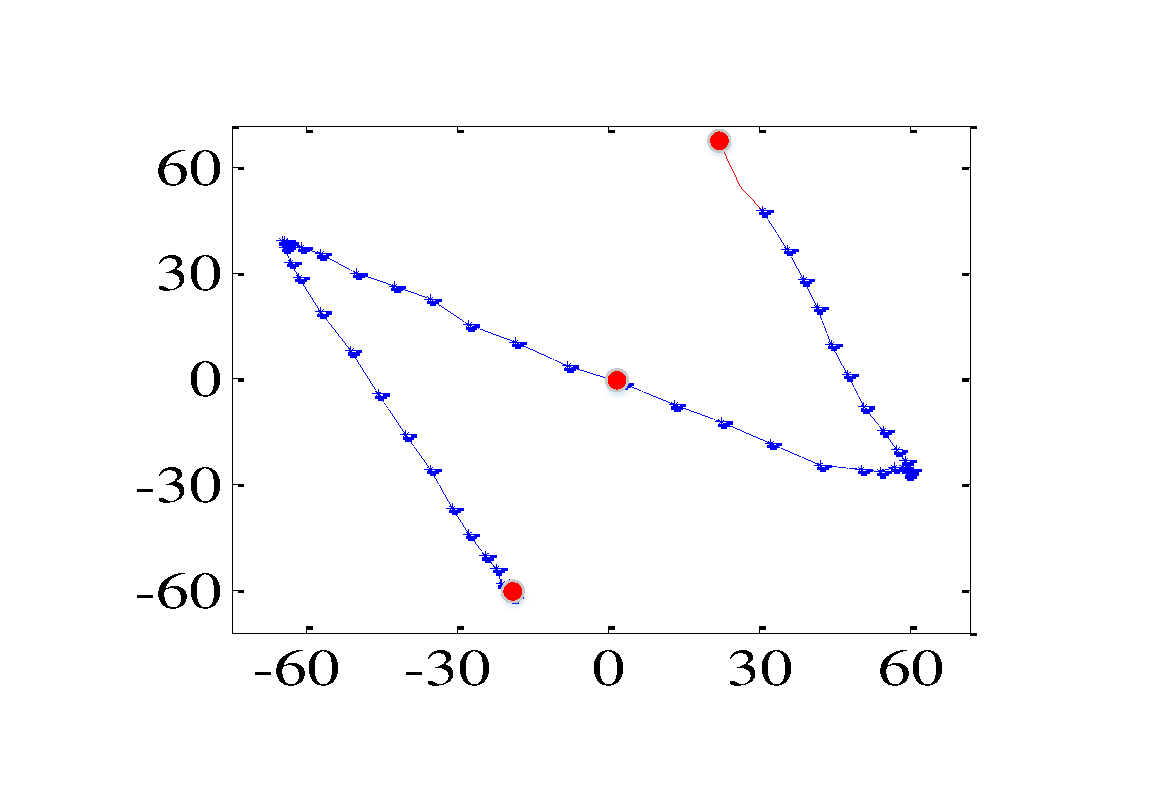
\includegraphics[width=1\textwidth]{fig/6--4.pdf}\\
                \centering  (d) Fingertip movement trajectory
                \end{minipage}
            }
            %\vspace{-3mm}
            \caption{Tracking the fingertip movement trajectory. For each video frame, the system tracks two areas: one surrounds the fingertip and the other covers the edge of the device.
            The fingertip position is determined by computing the relative coordinates of the central points of the two areas.
            The red points highlighted in the final results (d) are the touching points tracked from the three video frames.}
            \label{fig:fig5}
            %\vspace{-3mm}
        \end{figure*}

\section{Implementation Details}

\subsection{Video preprocessing \label{sec:identify}}
\label{section:recognition}
The first step of our attack is to identify the unlocking process from the
video footage. While all our
participants (see Section~\ref{section:locking patterns}) consider this as a straightforward manual task, we developed a \emph{simple yet effective} heuristic to automatically detect the video segment in some typical scenarios. Our heuristic is based on the following observations: (1) before or after
unlocking, users often pause for a few seconds; (2) two consecutive on-screen operations (e.g. swiping, zooming etc.) typically expose some spatial-temporal motion characteristics.
To test our hypothesis, we have recorded 50 video streams (where each
video stream lasts around 2 minutes) of how ten of our participants drew
patterns. During video recording, our participants firstly performed
some on-screen activities such as web browsing and gaming as they wished;
they then randomly opened up a pattern lock screen to draw a pattern and
continued to perform other on-screen operations afterwards.
We then analyzed frames that are associated with pattern drawing and those are not.


Figure~\ref{fig:time-interval} shows that all our participants paused at least $1.5$ seconds before or after pattern drawing due to delay of the user or the device.
%Our algorithm leverages this characteristic to locate the start and end point of unlocking process.
We also found that identical on-screen activities often follow closely. For example, on several occasions our participants had to swipe several times  to locate a program from the application list.
These consecutive on-screen operations have some spatial-temporal motion characteristics that are different from pattern drawing.
Figure~\ref{fig:gesture-distinction} shows the spatial-temporal motion structure for  two gestures, swiping and zooming, when they are performed once (a, c, e) and twice (b, d, f).
This diagram indicates that the spatial-temporal motion of two identical on-sreen activities contains one or more loop structures for which pattern drawing does not have.


Our heuristic is described
in Algorithm~\ref{alg:recognition}. The input to the algorithm is a video capturing the unlocking process, and the output of the
algorithm is a time-stamp tuple, $<$start, end$>$, which marks the start and the end
of a video segment.
To locate the video segment of pattern drawing, we first filter out on-screen activities where the
fingertip location does not change within a timeframe of 1.5 seconds (lines 4 and 11). This
allows us to exclude some basic on-screen activities, such as clicking. We
use the number of video frames, \emph{frameCount}, as a proxy to estimate the time interval. Here, a time
interval of 1.5s translates to 45 frames or 90 frames when the video was shot
at 30 or 60 frames per second (FPS) respectively. We also use the
spatial-temporal characteristics described above to exclude two consecutive swiping or zooming gestures (line 8). Finally, we exploit the observation that users
typically paused at least 1.5s before or after unlocking to locate the start
and end points of pattern drawing (line 19).

\noindent \textbf{Limitations} Our heuristic is likely to fail if the user was typing
using a Swype-like method (i.e. entering words by sliding a finger from
the first letter of a word to its last letter) during video recording. In
this case, our method will identify multiple video segments of which one may contain
the pattern unlock process. If multiple segments are detected, the algorithm will ask the
user to confirm which video segment to use.
In this scenario, the first identified segment is likely to be the correct one.
In practice, an experienced attacker would wait patiently to avoid this
complicated situation by finding the right time for filming (e.g. for a screen
lock, the time is just after the device is retrieved).
The attacker could also watch the video to manually cut it to ensure \FIXED{to} obtain the correct video segment.
It is
worthwhile to mention that automatically identifying the pattern unlocking process is
not central to our attack because an experienced attacker can watch the video to manually cut it to ensure the tracking algorithm (described in the section) receives a quality input.
Despite its limitations, our algorithm can reduce the efforts involved in some common scenarios.

\subsection{Track fingertip locations}
\label{section:tld}

        After cutting out the video segment of pattern drawing, we need to track the finger motions from the video segment. We achieve this by employing a video tracking algorithm called
        \emph{Tracking-Learning-Detection (TLD)}~\cite{kalal2012tracking}. This
        algorithm automatically detects objects defined by a boundary box. In
        our case, the objects to be tracked are the user's fingertip and an area of the device.
        These are supplied to the algorithm by simply highlighting two areas on the first frame of the video segment (see Figure~\ref{fig:fig2} b). The
        algorithm tries to localize the fingertip from each video frame and aggregates the successfully tracked locations to produce a fingertip movement trajectory as an output (see Figure
        \ref{fig:fig2} c).

    \subsubsection{Generate The Fingertip Movement Trajectory}

        The TLD algorithm automatically detects
        objects based on the examples seen from the first frame.
        For each tracked object, the algorithm generates a confidence between 0 and 1.
        A tracking is considered to be successfully if the confidence is greater than a threshold.
        In our experiments, this threshold is set to 0.5 since this value is found to give good performance in our initial design experiments using 20 patterns\footnote{To provide a fair evaluation, the patterns used in
        our initial test runs in
        the design phase are different from the ones used later in evaluation.}.
        TLD has three modules: (1) a tracker that follows
        objects across consecutive frames under the assumption
        that the frame-to-frame motion is limited and objects are visible;
        (2) a detector to fully scan each individual frame to localize all
        appearances of the objects that have been seen in previous frames; and
        (3) a learner that estimates errors of the detector and updates the detector to avoid these errors in future
        frames.


        The TLD learner automatically extracts features from the area of interest to build a K-Nearest Neighbor
        classifier~\cite{hastie1996discriminant}
        which is a part of the detector. In the following frames, the learner
        estimates the detection errors and generates new training
        examples (i.e. new appearances of the object) arose from object motion to
        re-train the classifier to avoid these errors. For each video frame,
        TLD calculates the tracking confidence and if the confidence is lower than the predefined threshold, the result of
        this particular frame will be discarded. This allows the algorithm to
        tolerate a certain degree of detection errors. Finally, the
        successfully detected object locations will be put onto a single
        image as the output. Detailed discussion of TLD can be found
        at~\cite{kalal2012tracking}.
        Sometimes the algorithm may fail to detect the objects in many video frames due to poor selections of interesting areas. If this happens, our system will ask the user to re-select the areas to track.
        We have also extended TLD to report when a
        fingertip position is seen on the footage. This temporal information is recorded as the number
        of video frames seen so far. This
         is used to separate two possibly overlapping line segments described in Section~\ref{section:spea}.

        \begin{figure*}[!t]
        \centering
        \subfigure{
            \begin{minipage}[b]{0.24\textwidth}
            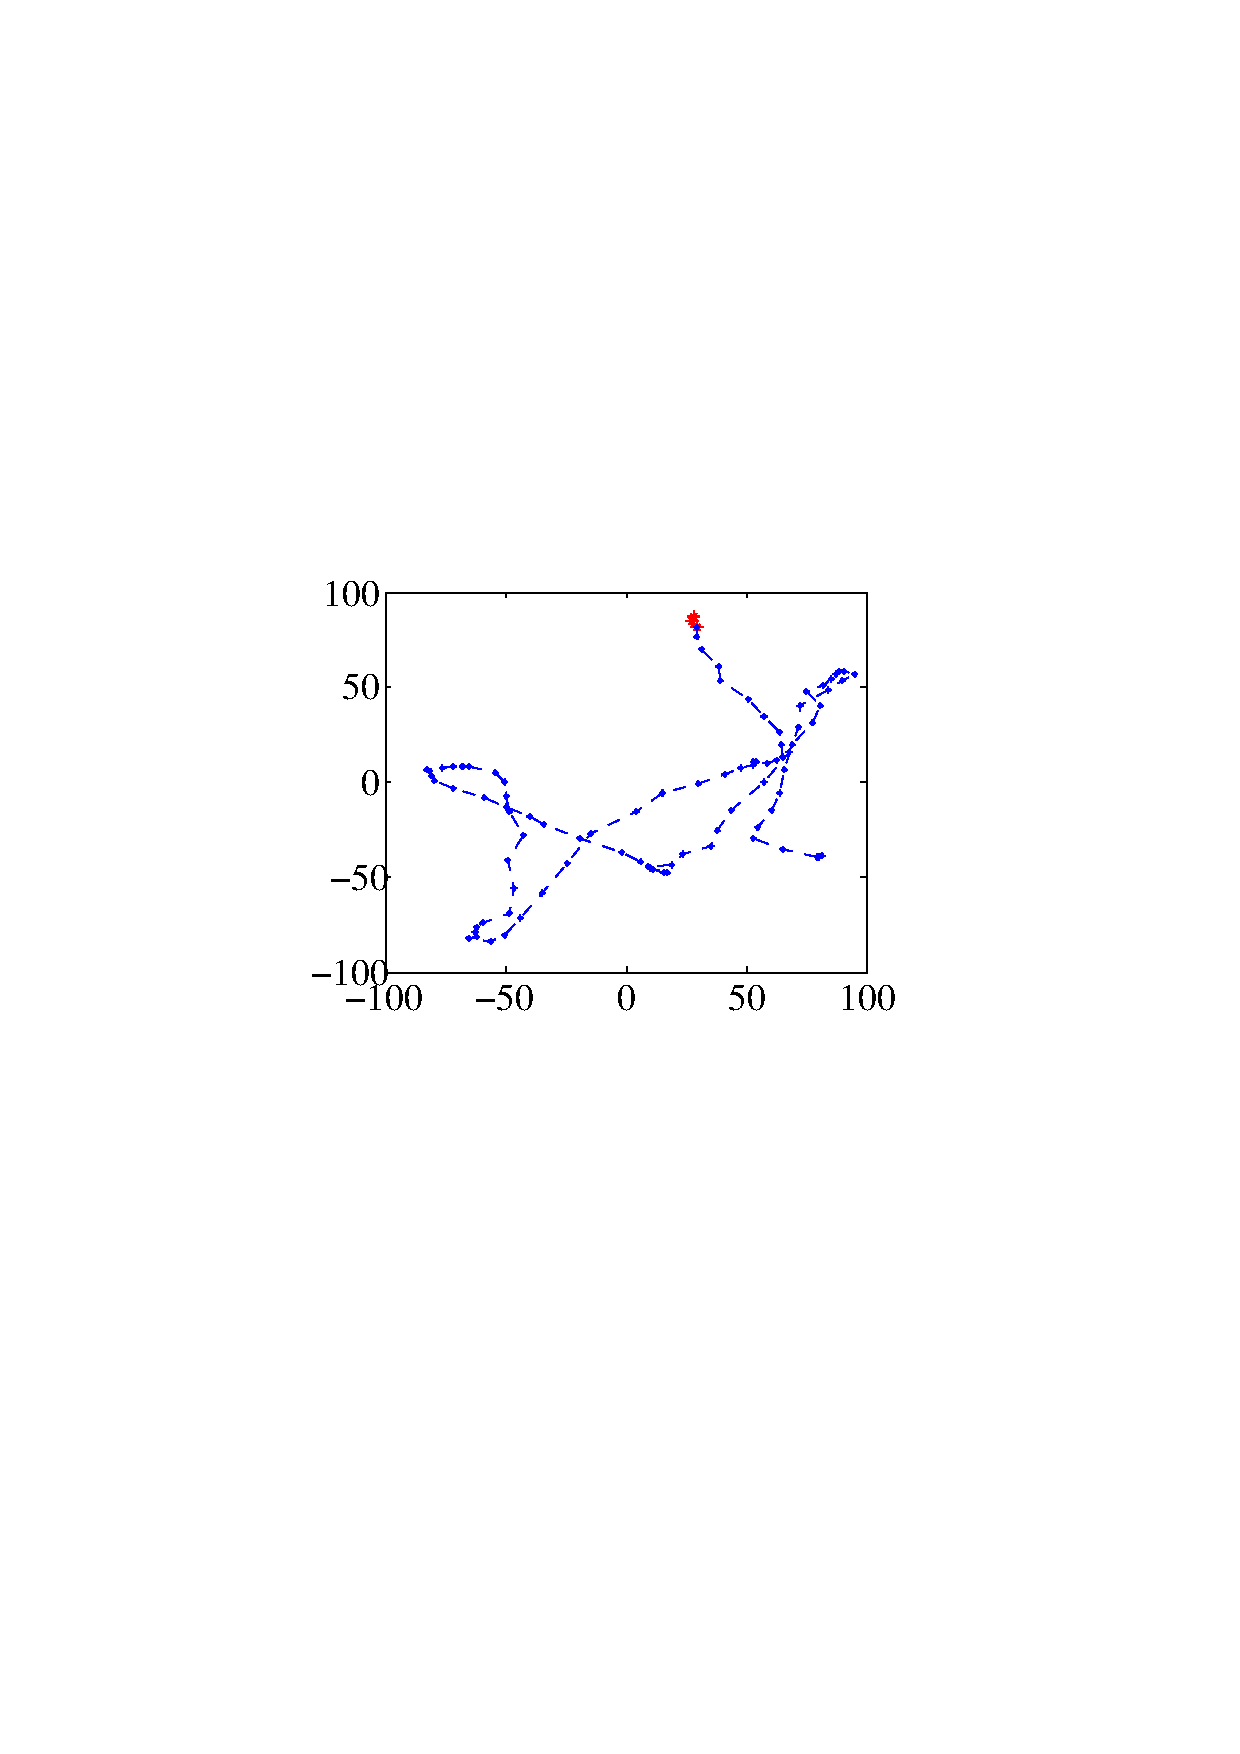
\includegraphics[width=\textwidth]{fig/5-1.pdf}\\
            \centering  (a) w/o camera shake calibration
            \end{minipage}
        }
        \hfill
        \subfigure{
            \begin{minipage}[b]{0.24\textwidth}
            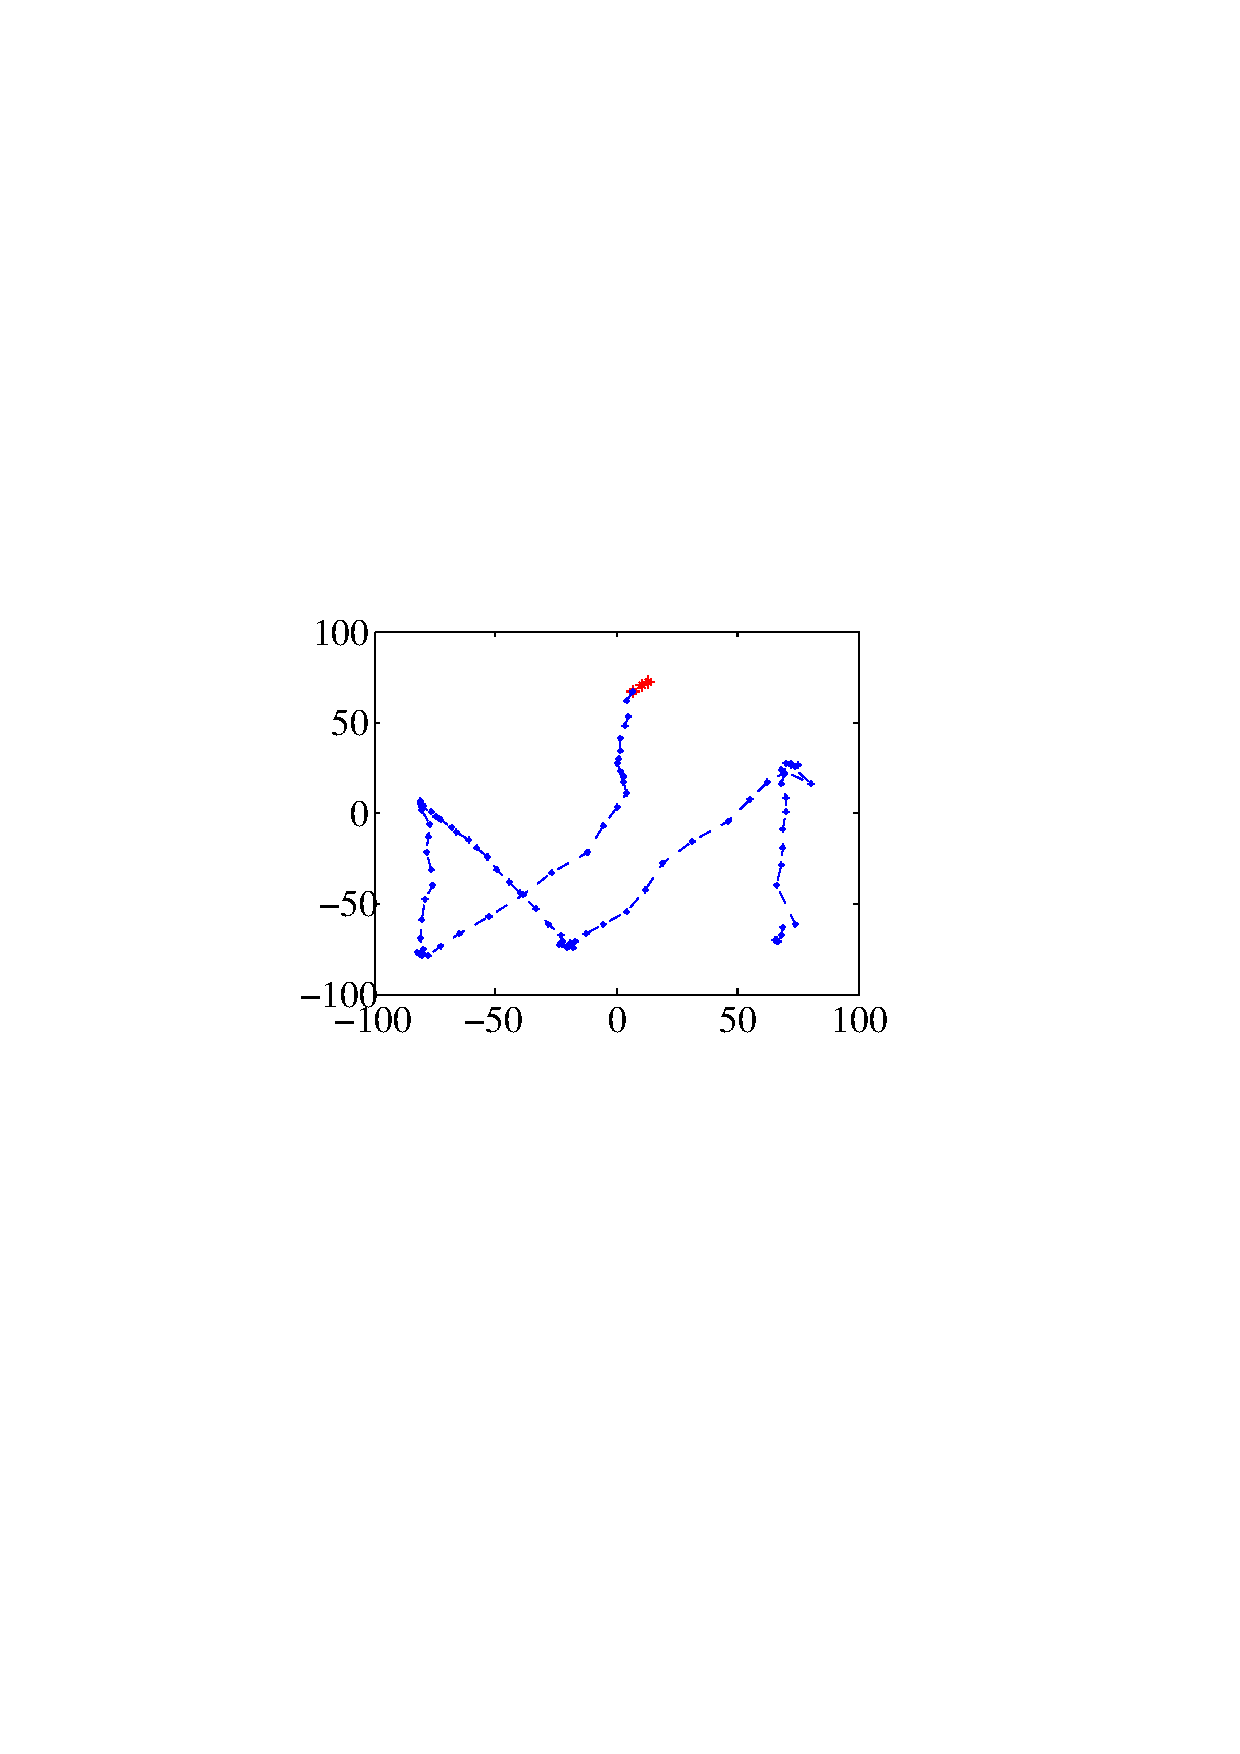
\includegraphics[width=\textwidth]{fig/5-2.pdf}\\
            \centering  (b) w/ camera shake calibration
            \end{minipage}
        }
        \hfill
        \subfigure{
            \begin{minipage}[b]{0.18\textwidth}
            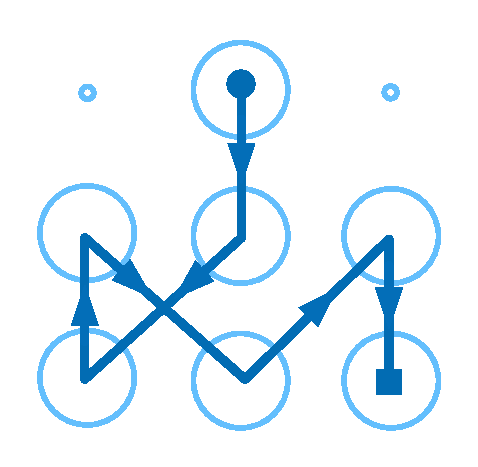
\includegraphics[width=\textwidth]{fig/5-3.pdf}\\
            \centering  (c) correct pattern
            \end{minipage}
        }
        %\vspace{-3mm}
        \caption{The resulted fingertip movement trajectories without (a) and with (b) camera-shake calibration.  The correct pattern is shown in (c). To aid clarity we have transformed (a) and (b) to the user's perspective.}
        \label{fig:camera_shake_illu}
         \end{figure*}

\begin{figure}[!t]
    \centering
    
\includegraphics[width=0.45\textwidth]{fig/line_detection.pdf}
    \caption{Filming angle calculation. The filming angle, $\theta$, is the angle between the edge line of the device and a vertical line.}
    \label{fig:line_detection}
\end{figure}

        \subsubsection{Camera Shake Calibration}
        \label{secction:shake}
         By default, the TLD algorithm reports the position of a tracked object with respect to the top-left pixel of the video frame.
         However, videos recorded by a hand-held device are not always perfectly steady due to
        camera shake. As a result, the top-left pixel of a video frame may appear in a different location in later frames.
        This can drastically affect the precision of fingertip localization, leading to misidentification of patterns.

        Our approach to cancel camera shake is to record the fingertip
        location with respect to a fixed point of the target device. To do so, we track two
        areas from each video frame. One area is an edge of the device and
        the other is the fingertip. Both areas are highlighted on the
        first frame by the user.
        The location of a successfully tracked fingertip is reported as
        the relative coordinates of the two center points of the marked areas.
        This approach can also be used to calibrate the slight movements of the target device when drawing the pattern.

        \noindent \emph{Example:} To illustrate how our camera-shake calibration method  works, considering
        Figure~\ref{fig:fig5} where two areas are firstly marked by two
        bounding boxes in subfigure (a).
        Both areas will
        then be automatically detected by the TLD algorithm in following video
        frames as shown in subfigures (b) and (c).
        The coordinates of the two center points of each box are the values of $x$ and $y$, and their relative positions are represented by
        $\triangle X$ and $\triangle Y$.
        For each frame
        where both areas are successfully tracked, we
        compute the relative coordinates, ($\triangle X$, $\triangle Y$), which are reported as the location of the tracked fingertip.

        Figure~\ref{fig:camera_shake_illu} shows the results when using TLD to process a video that was filmed with some camera shake effects.
        Here we show the results without (Figure~\ref{fig:camera_shake_illu} a) and with (Figure~\ref{fig:camera_shake_illu} b) camera-shake calibration. To aid clarity, we have
        converted the trajectories into the user's perspective. Without
        camera-shake calibration, the resulted trajectory is significantly different from the actual pattern shown in Figure~\ref{fig:camera_shake_illu} (c).
        Because of this great difference, using Figure~\ref{fig:camera_shake_illu} (a)  will lead to misidentification of
        candidate patterns. By contrast, processing the same video
         with camera-shake calibration  produces Figure~\ref{fig:camera_shake_illu} (b). Clearly, this figure is more
        alike the correct pattern.

        \subsubsection{Noisy Points Calibration}
            During tracking process, the TLD algorithm may report mistaken position of a tracked object as rapid deformation of the tracked object. This can affect the shape of fingertip movement, leading to extract \FIXED{incorrect} geometric information of fingertip movement.

\subsection{Filming angle transformation}
\label{sec:transformation}
In practice, the filming camera will not directly face the target device to avoid the filming activity to be noticed by the user. As a result, the
fingertip movement trajectory generated by the tracking
algorithm will look differently from the actual pattern. For example, for the
pattern presented in Figure~\ref{fig:fig2} (a), if the video is filmed from the attacker's front-left to the target device (i.e. with a filming angle of approximate 45 degrees),
we get the trajectory shown in Figure~\ref{fig:fig2} (c).
Using this trajectory without any postprocessing will lead to misidentification of candidate patterns.
Therefore, we must transform the resulted trajectory to the user's view point. To do so, we need to estimate the angle between the filming camera and the target device. Our approach is described as follows.

We use an edge detection algorithm called Line Segment Detector (LSD)~\cite{grompone2010lsd} to detect the longer edge of the device.
The filming angle is the angle between the detected edge line and a vertical line. This is illustrated in Figure~\ref{fig:line_detection}.
In Section~\ref{sec:angle}, we show that a slight estimation error of the filming angle has little impact on the success of the attack.
By default, we assume that the pattern grid is presented in the portrait
mode\footnote{The pattern grid of the Android native pattern lock is always presented in the portrait mode regardless of the orientation of the device.}. If this is
not the case, i.e. the pattern grid is shown in the landscape mode, we need
to use the shorter edge of the device to calculate the filming angle. We believe that an attacker interested in a particular target would
have some knowledge of how the pattern grid of the target device is presented under different orientation modes and be able to identify the device orientation by watching the video.
There are also other methods to be used to identify the filming angle~\cite{Torralba:2002:DEI:628330.628820}.


Based on the estimated filming angle, $\theta$, we use the following formula to transform the tracked fingertip movement trajectory from the camera's view point to the user's:

\begin{equation}
        S=TS^{'} \qquad, \qquad  T=\left[ \begin{matrix} \cos\theta & -\sin\theta \\ \sin\theta & \cos\theta \end{matrix} \right]
\end{equation}

where $T$ is a Transformation Matrix, $S^{'}$ is the coordinate of a point of the tracked trajectory, and $S$ is the resulted coordinate after the transformation.
For each video frame, our algorithm individually calculates the filming angle and performs the transformation, because the filming angle may change across video frames.


\subsection{Identify and rank candidate patterns}
\label{section:spea}
  In this step, the fingertip movement trajectory will be mapped to a number of candidate patterns to be tested on the target device.
   Our goal in this step is to exclude as many patterns as possible and only leave the most-likely patterns to be tried out on the target device.
     Our approach is to use the geometry information of the fingertip movement trajectory, i.e. the length and direction of line segments and the number of turning points, to reject patterns that do not satisfy certain criteria.
    In this section, we first describe how to identify overlapping line segments and extract length and direction information before presenting how to use the extracted information to identify and rank candidate patterns.

    \begin{figure}[!t]
        \centering
        \subfigure{
            \begin{minipage}[b]{0.23\textwidth}
            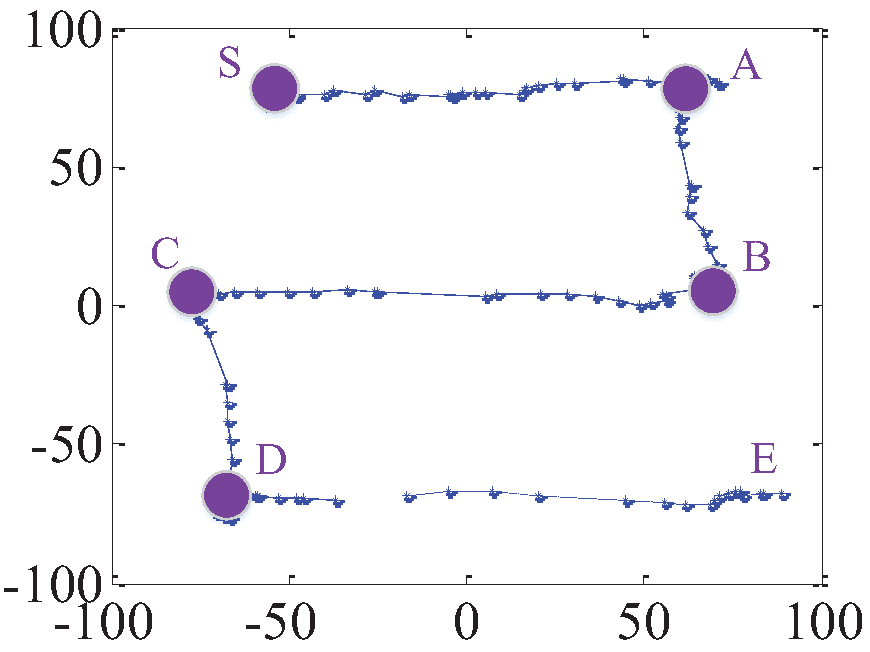
\includegraphics[width=\textwidth]{fig/6-2.pdf}\\
            \centering  (a) tracked fingertips
            \end{minipage}
        }
        \hspace{0.2cm}
        \subfigure{
            \begin{minipage}[b]{0.18\textwidth}
            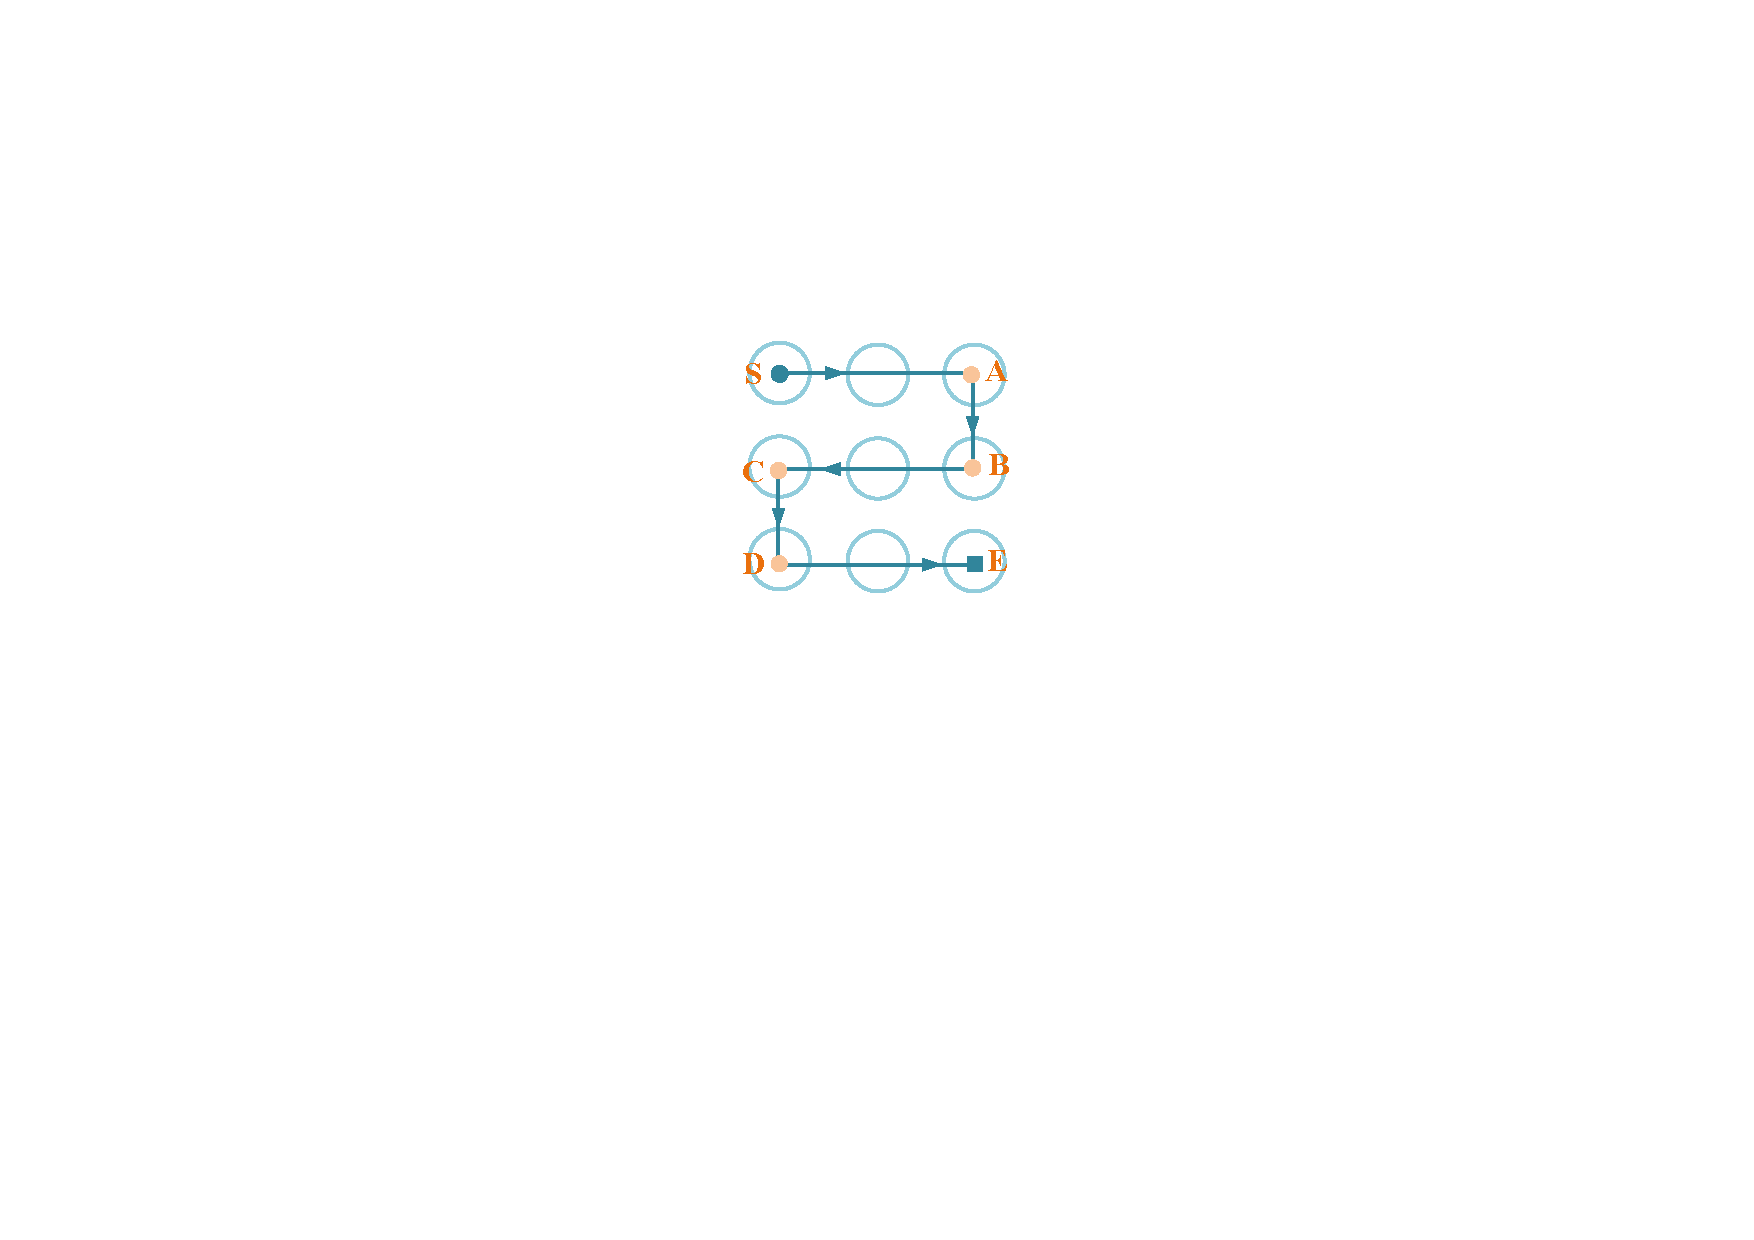
\includegraphics[width=\textwidth]{fig/6-1.pdf}\\
            \centering  (b) pattern example
            \end{minipage}
        }
        \caption{This figure shows the tracked fingertip movement trajectory (a) of a pattern (b). Point S on (a) is the starting point and points A, B, C, and D on (b) represent four turning points.}
        \label{fig:fig6}
    \end{figure}

\renewcommand{\algorithmicforall}{\textbf{for each}}
    \begin{algorithm}[!t]
        \caption{Line Segment Identification}
        \label{alg:turning-point}
        \begin{algorithmic}[1]
            \REQUIRE~~\\
                \textbf{struct} $T[]$: Temporal information of each tracked location\\
                $timeTh$: Threshold of whether two line segments are overlapping \\
            \ENSURE~~\\
                $tp[]$ Turning points of fingertip movement. \\
            \FOR{\textbf{each} fingertip movement with temporal sequences $T[]$}
                \STATE $tpNum=0$; \\
                \STATE \textbf{struct} $lines[] \leftarrow getLines(T[]) $ \\
           % \FOR{\textbf{each} t in $T[]$}
                \STATE $lNum \leftarrow getLinesNumber(lines[])$ \\
                \FOR{$i=1:lNum$}
                    %\STATE $tp[tpNum] \leftarrow getStartingPoints(lines[i],timeTh)$ \\
                    \IF{$checkOverlap(lines[i],timeTh)$}
                        \STATE $p[tpNum++] \leftarrow getOverlapPoints(line[i])$ \\
                    \ENDIF
                    \STATE $p[tpNum++] \leftarrow getTurningPoints(line[i])$ \\
                \ENDFOR
            \ENDFOR
            \STATE $tp[]=p[0:end-1]$\\
        \end{algorithmic}
    \end{algorithm}

    \subsubsection{Extracting Structure Information}
        A pattern can be defined as a collection of line
        segments where each line segment has two properties:
        the length of the line, $l$, and the direction of the line, $d$. Figure~\ref
        {fig:fig7} shows all the possible directions of a $3 \times 3$ pattern grid.
        We define a
         pattern, $P$, as a collection of line segment prosperities,  $P=\{L, D\}$.
        Here $L=\{l_{1}, l_{2}, \cdots, l_{n}\}$ is a collection of the lengths
        of all line segments (that are numbered from $1$ to $n$) of the pattern, and $D=\{d_{1}, d_{2}, \cdots, d_{n}\}$ is the collection of directions for all line segments in $L$.
        Algorithm~\ref{alg:alg1} describes how $P$ is extracted.
        We extract the length and the direction of each line segment from the tracked fingertip movement trajectory and store them
        into arrays $L[]$ and $D[]$ respectively.

        \begin{figure}[!t]
            \centering
            \subfigure{
                \begin{minipage}[b]{0.35\textwidth}
                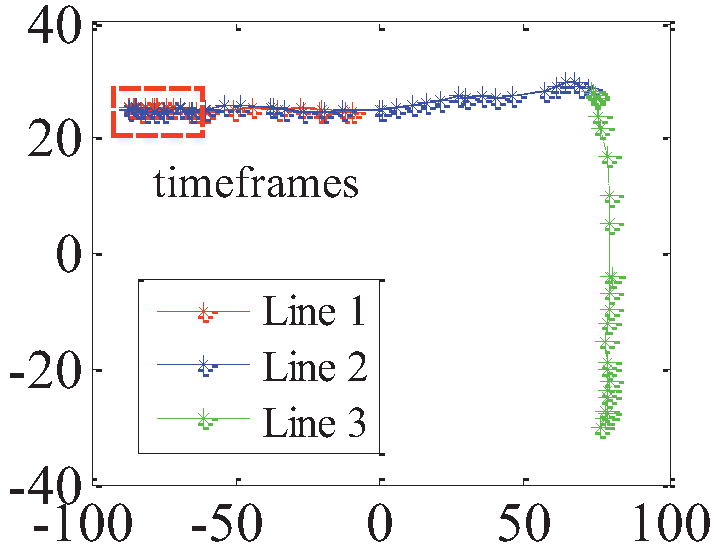
\includegraphics[width=\textwidth]{fig/line-identification1.pdf}\\
                \centering  (a) overlapping lines
                %\FIXME{Need to mark the starting point and turning point}
                \end{minipage}
            }
            \hfill
            \subfigure{
                \begin{minipage}[b]{0.35\textwidth}
                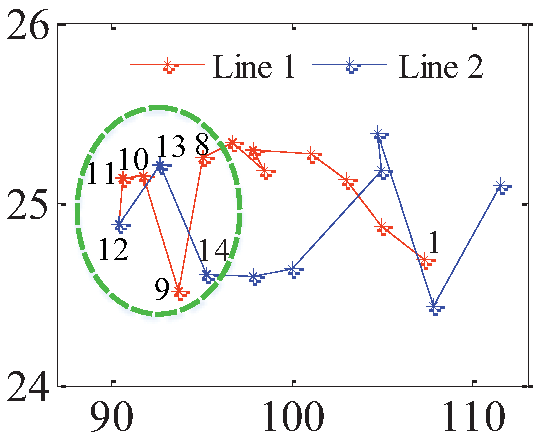
\includegraphics[width=\textwidth]{fig/line-identification2.pdf}\\
                \centering  (b) zoom-in view
                \end{minipage}
            }
            \caption{Separating two overlapping line segments by checking the number of overlapping points within a timeframe.}
            \label{fig:line-idenfication}
        \end{figure}

        \begin{figure}[!t]
            \centering
            \subfigure{
                \begin{minipage}[t]{0.3\textwidth}
                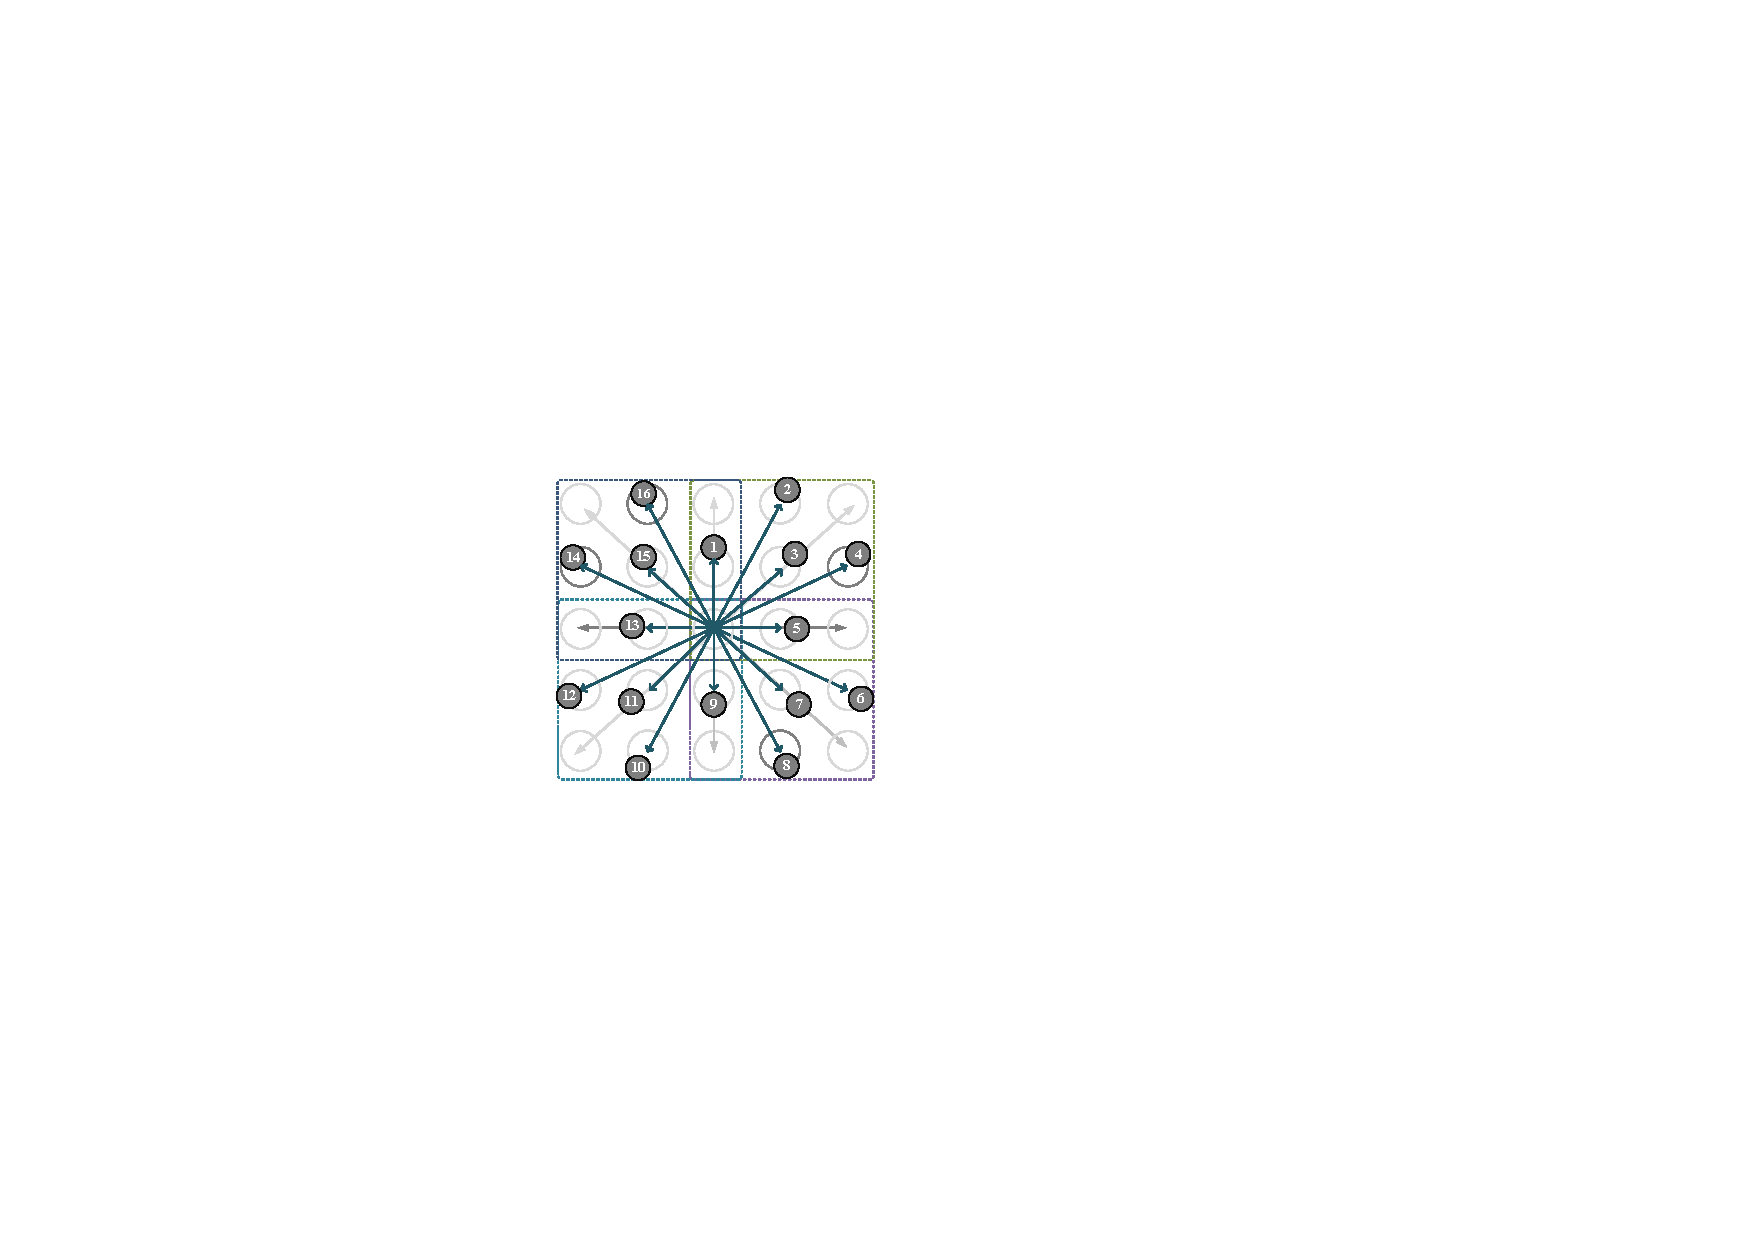
\includegraphics[width=\textwidth]{fig/7-1.pdf}\\
                \centering (a) line direction number
                \end{minipage}
            }
            \subfigure{
                \begin{minipage}[t]{0.35\textwidth}
                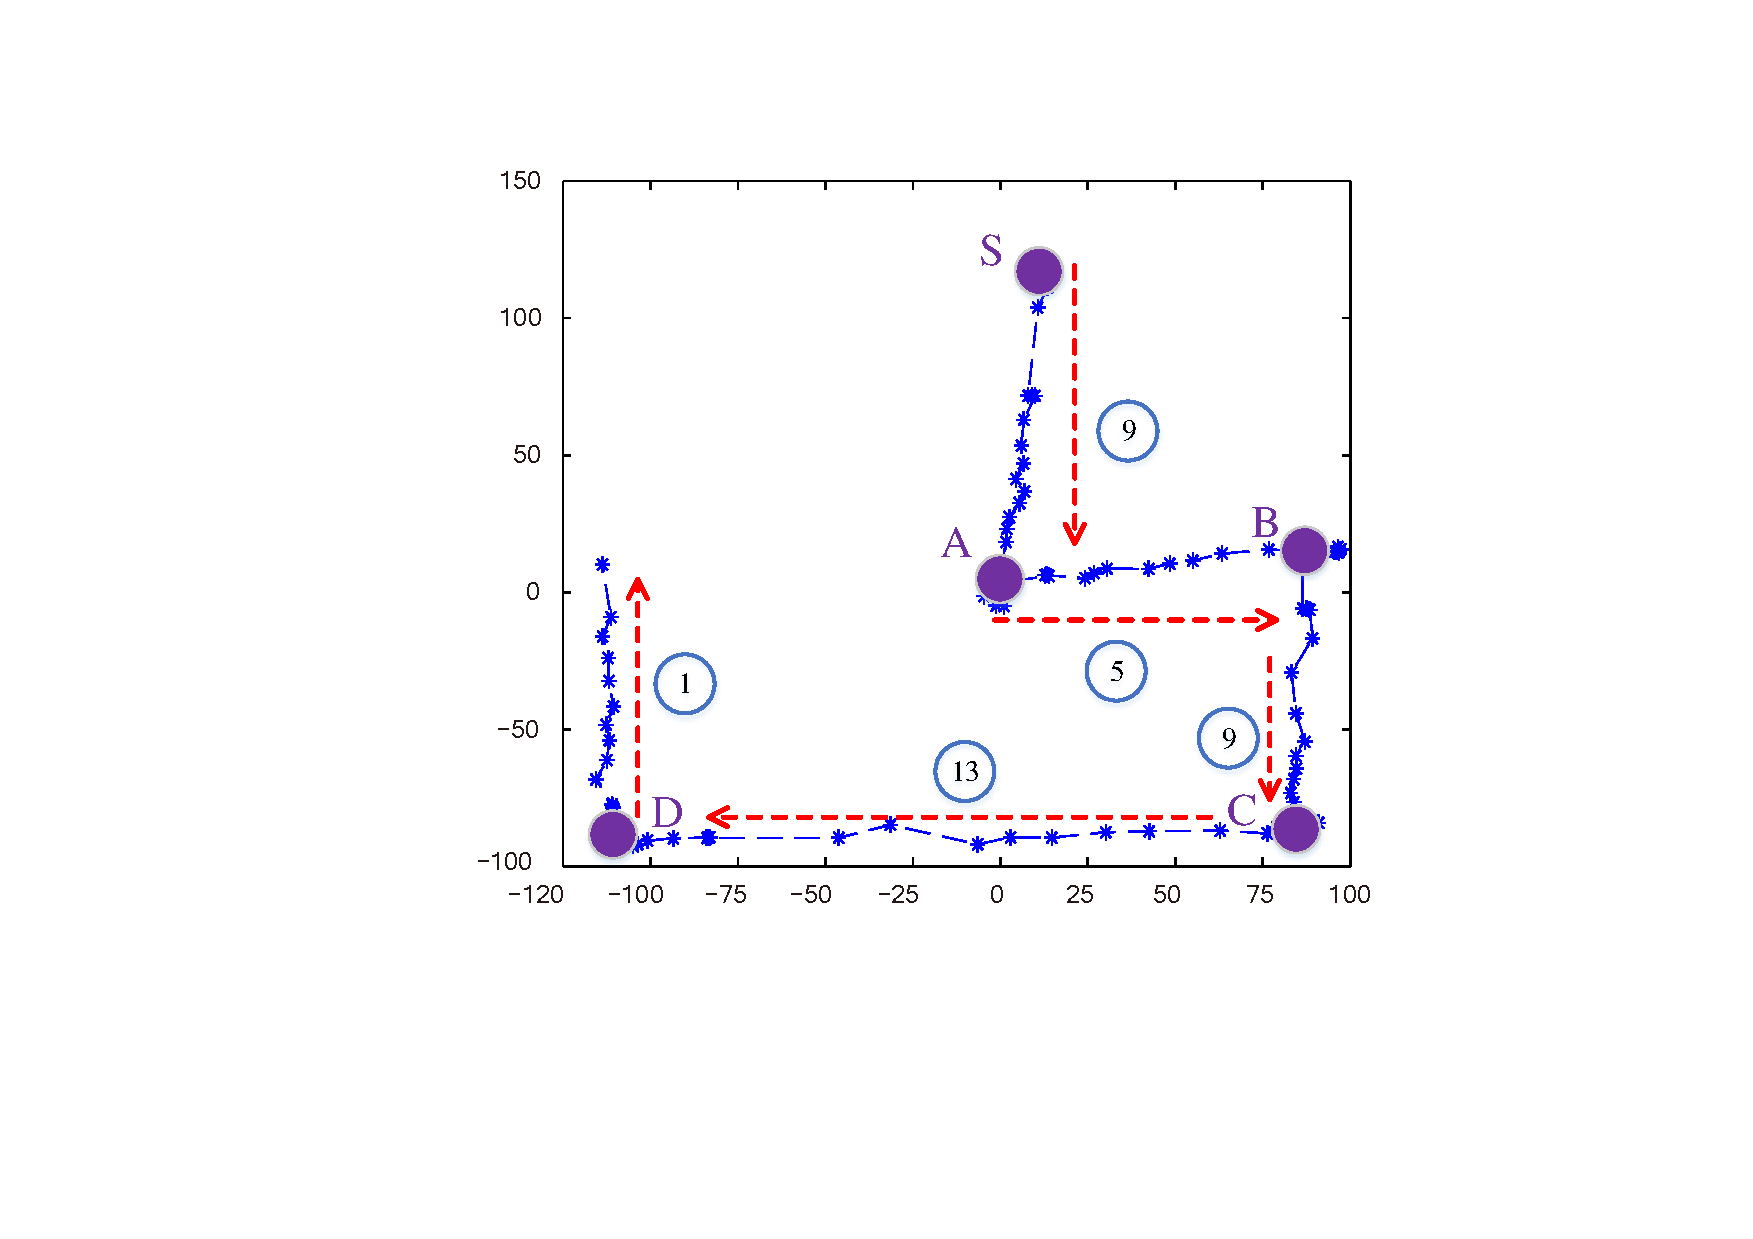
\includegraphics[width=\textwidth]{fig/7-2.pdf}\\
                \centering (b) numbering line segment of the tracked trajectory
                \end{minipage}
            }
            \caption{All possible line directions on a $3 \times 3$ Android pattern grid (a) and an example trajectory (b).}
            \label{fig:fig7}
        \end{figure}

        \vspace{2mm}
        \noindent \textbf{Identify Line Segments.}
        The first step of geometry information extraction is to identify individual
        line segments from the trajectory. This can be achieved
        by finding turning points, the start and the end points of the pattern, because two points define a line segment. For example, turning points, A and B, in
        Figure~\ref{fig:fig6} defines a line segment, AB. In
        Algorithm~\ref{alg:turning-point}, we use a linear fitting
        method~\cite{Kutner2004Applied} to discover turning points (line 3). A specific
        challenge here is how to separate two overlapping line segments (see
        Figure~\ref{fig:intersection-overlap} c for an example).
        It is to note that up to two lines can be overlapped on a pattern grid.
        The naive
        linear fitting algorithm would consider two overlapping segments to be a
        single line as their points stay close to each other. We overcome this problem
       by using the temporal information (that is recorded by the
        tracking algorithm) to separate two overlapping points.
        To do so, we visit all tracked points of each line segment given by the linear fitting algorithm (line
        5) within a timeframe (\emph{timeTh}) of 20 video frames for a video of 30 FPS (40 for a video of 60 FPS).
        For each point, we calculate its Euclidean distances to all other points within the timeframe.
        We consider two points to be overlapping if their distance is less than 5 pixels.
        For a video shot at 30 FPS, we consider there exist two overlapping line segments if 5 (10 for a 60 FPS video) or more overlapping points in the timeframe.
        Again, these threshold values were determined through our initial design experiments.
        Finally, we consider the center of all points as the turning point of the two overlapping line segments and use turning point to separate the two lines.

        \noindent \emph{Example:} As an example, consider a fingertip movement trajectory shown in
        Figure~\ref{fig:line-idenfication} (a). The red rectangle on the
        figure is a timeframe consisting of 20 tracked points.  If we zoom in
        on the timeframe, we get Figure~\ref{fig:line-idenfication} (b) where
        a point is labelled with a frame number according to when
        the point was seen, starting from 1 for the earliest point. In this example, there are more than 6
        overlapping points in the timeframe, which are marked by a green
        circle. We use the center
        point (No.10) of the overlapping points as the turning point to separate the two line segments.

        \begin{table}[!t]
            \centering
            \caption{Mappings from line slopes and fingertip-horizontal movements to direction numbers}
            \label{tab:slopes}
            \small
            \begin{tabular}{lcccccccc}
                \toprule
                \textbf{Direction No.}& 1 & 2 & 3 & 4 & 5 & 6 & 7 & 8 \\
                \textbf{slope (L $\rightarrow$ R)} & $+\infty$ & $2$ & $1$ & $\frac{1}{2}$ & $0$ & $-\frac{1}{2}$ & $-1$ & $-2$ \\
                \midrule
                \textbf{Direction No.}& 9 & 10 & 11 & 12 & 13 & 14 & 15 & 16 \\
                \textbf{slope (R $\rightarrow$ L)} & $-\infty$ & $2$ & $1$ & $\frac{1}{2}$ & $0$ & $-\frac{1}{2}$ & $-1$ & $-2$ \\
                \bottomrule
            \end{tabular}
            \vspace{-2mm}
        \end{table}

\renewcommand{\algorithmicforall}{\textbf{for each}}
    \begin{algorithm}[!t]
        \caption{Candidate Pattern Identification Algorithm}
        \label{alg:alg1}
        \begin{algorithmic}[1]
            \REQUIRE~~\\
                $L[]$: Relative line length \\
                $D[]$: Direction number (see Figure~\ref{fig:fig7}) \\
                $tn$: Number of turning points of fingertip trajectory \\
                %$timeTh$ Threshold of considering the turning points.\\
                $lengthTh$: Threshold of considering two lines to have the same length\\
                $directionTh$: Threshold of considering two lines to be in the same direction\\
            \ENSURE~~\\
                $P[]$: Candidate patterns \\

            \FOR{\textbf{each} possible pattern $p$ with $tn$ turning points}
                \STATE $n \leftarrow getLineNumber(P[])$ \\
                \STATE $pL[]  \leftarrow getRelativeLength(p)$ \\
                /*Relatvie line length for pattern $p$*/ \\
                \STATE $pD[] \leftarrow getDirection(p)$ \\
                \IF{match($pL[]$, $L[]$, $lengthTh$)}
                    \IF{match($pD[]$, $D[]$, $directionTh$)}
                        \STATE $P[] \leftarrow p$\\
                    \ENDIF
                \ENDIF
            \ENDFOR
            \STATE $P[] \leftarrow sort(P[])$
        \end{algorithmic}
    \end{algorithm}

        \vspace{2mm}
        \noindent \textbf{Extract the Line Length.}
        The physical length of a line segment depends
        on a number of device-specific parameters: the sizes of the screen and the pattern grid, and the space between two touch dots.
        To ensure our approach is independent of the device, we normalize the physical length of a line segment to the
        shortest line found on the tracked trajectory. For the
        example shown in Figure~\ref{fig:fig6} (a), the line lengths for segments, SA, AB, BC, CD, and DE, are $2l_{s},l_{s},2l_{s},l,2l_{s}$, respectively.
        Here segments AB and CD have the shortest length, $l_s$. The physical length of a line segment is calculated by computing the
        Euclidean distance between the start and the end points of a segment.

        \vspace{2mm}
       \noindent \textbf{Extract Direction Information.}
       In addition to the line length, we also want to know to which
       direction the finger moves. This information is useful for inferring which dots are selected to unlock the pattern.
       Figure~\ref{fig:fig7} (a) shows all possible 16
        directions on a $3 \times 3$ pattern grid. The
        directions are numbered from 1 to 16 in clockwise.
        For each line segment of the tracked trajectory, we calculate its line slope and the horizontal movement of the finger (i.e. left $\rightarrow$ right or vice versa).
        This information will then be checked against Table~\ref{tab:slopes} to determine the direction number of the line segment.
         The horizontal movement of the fingertip is determined by first using the temporal information to find out the start and the end points of the line and then comparing the horizontal coordinates of the two points.
        The line slope is also computed based on the coordinates of the
       start and the end points of the
        line segment.
        Figure~\ref{fig:fig7} (b) gives the direction number of each
        tracked line segment of a fingertip movement trajectory.

\begin{figure}[!t]
        \centering
        \subfigure{
            \begin{minipage}[b]{1.3cm}
            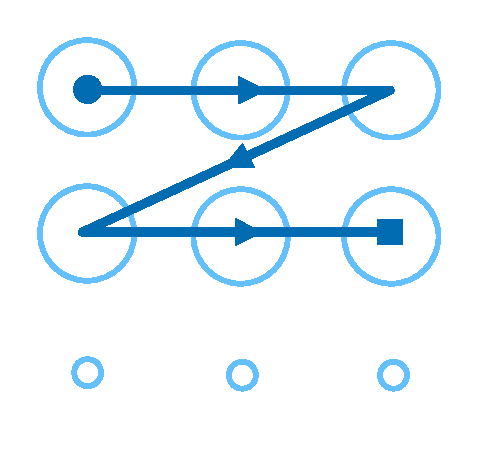
\includegraphics[width=1.3cm]{fig/600.pdf}\\
            \centering  a(1)
            \end{minipage}
        }
        \hspace{-0.2cm}
        \subfigure{
            \begin{minipage}[b]{1.3cm}
            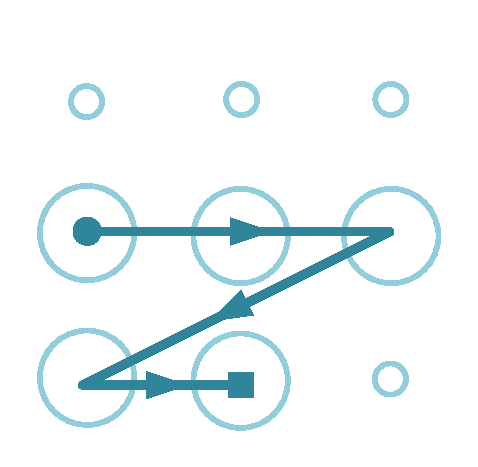
\includegraphics[width=1.3cm]{fig/601.pdf}\\
            \centering  a(2)
            \end{minipage}
        }
        \hspace{-0.2cm}
         \subfigure{
            \begin{minipage}[b]{1.3cm}
            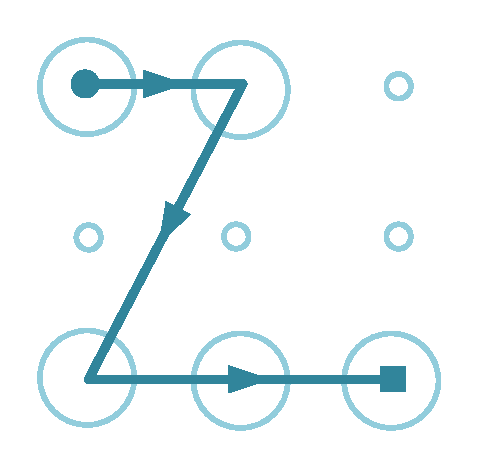
\includegraphics[width=1.3cm]{fig/602.pdf}\\
            \centering  a(3)
            \end{minipage}
        }
        \hspace{-0.2cm}
         \subfigure{
            \begin{minipage}[b]{1.3cm}
            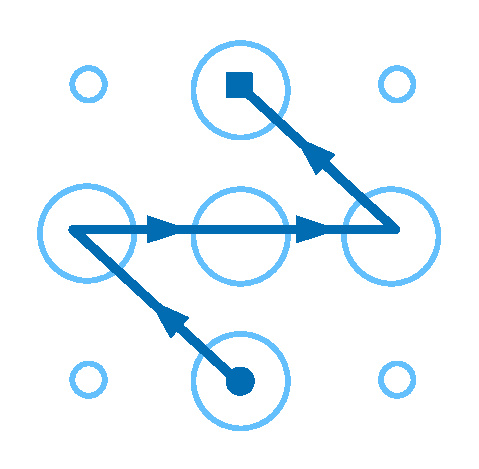
\includegraphics[width=1.3cm]{fig/603.pdf}\\
            \centering  a(4)
            \end{minipage}
        }
        \hspace{-0.2cm}
         \subfigure{
            \begin{minipage}[b]{1.3cm}
            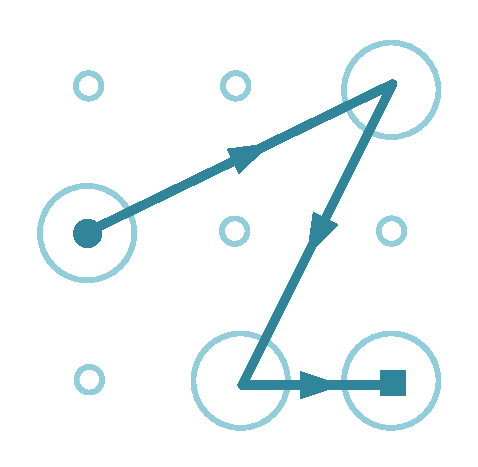
\includegraphics[width=1.3cm]{fig/604.pdf}\\
            \centering  a(5)
            \end{minipage}
        }
        \hspace{-0.2cm}
         \subfigure{
            \begin{minipage}[b]{1.3cm}
            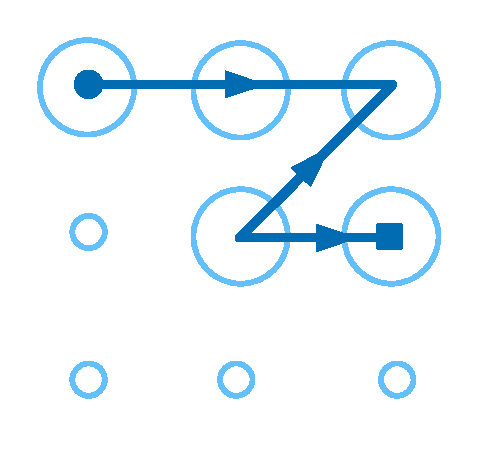
\includegraphics[width=1.3cm]{fig/605.pdf}\\
            \centering  b(1)
            \end{minipage}
        }
        \hspace{-0.2cm}
         \subfigure{
            \begin{minipage}[b]{1.3cm}
            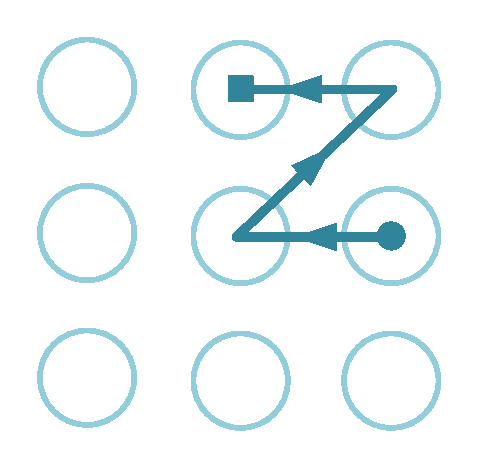
\includegraphics[width=1.3cm]{fig/606.pdf}\\
            \centering  b(2)
            \end{minipage}
        }
        \hspace{-0.2cm}
         \subfigure{
            \begin{minipage}[b]{1.3cm}
            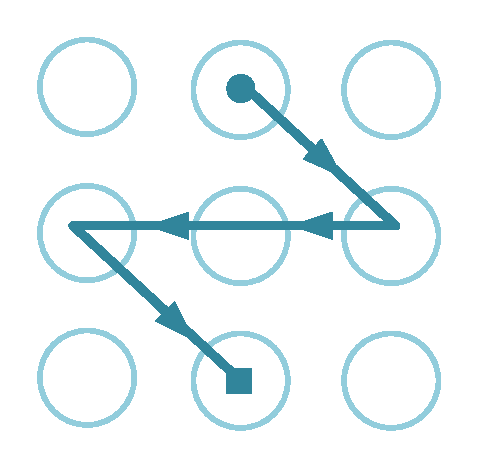
\includegraphics[width=1.3cm]{fig/607.pdf}\\
            \centering  b(3)
            \end{minipage}
        }
         \hspace{-0.2cm}
         \subfigure{
            \begin{minipage}[b]{1.3cm}
            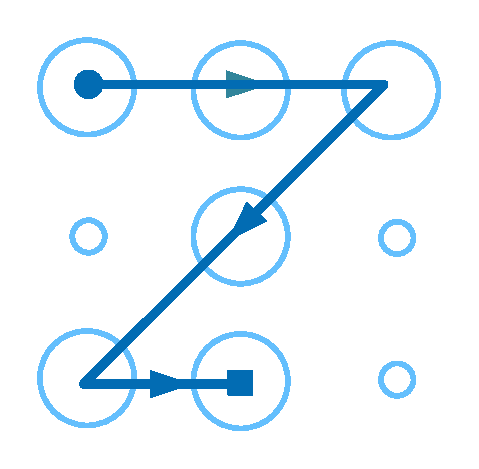
\includegraphics[width=1.3cm]{fig/608.pdf}\\
            \centering b(4)
            \end{minipage}
        }
         \hspace{-0.2cm}
         \subfigure{
            \begin{minipage}[b]{1.3cm}
            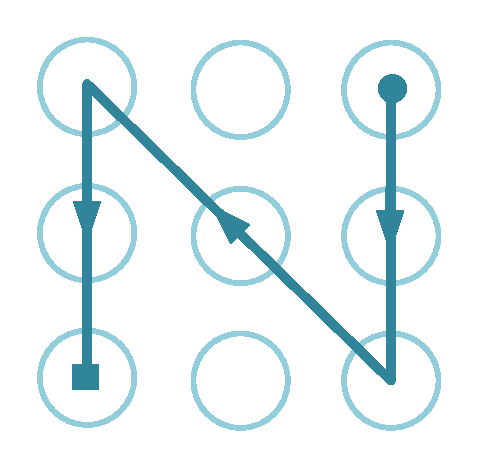
\includegraphics[width=1.3cm]{fig/609.pdf}\\
            \centering b(5)
            \end{minipage}
        }
         \hspace{-0.2cm}
         \subfigure{
            \begin{minipage}[b]{1.3cm}
            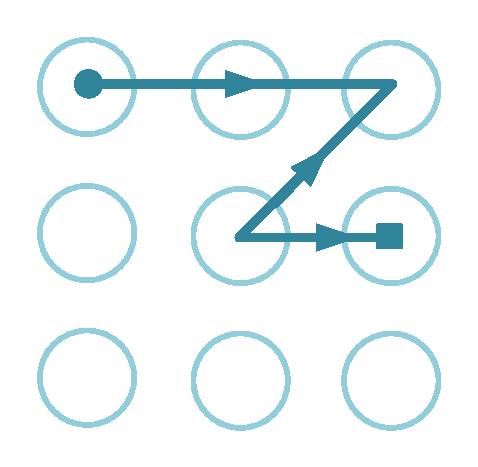
\includegraphics[width=1.3cm]{fig/610.pdf}\\
            \centering  c(1)
            \end{minipage}
        }
         \hspace{-0.2cm}
         \subfigure{
            \begin{minipage}[b]{1.3cm}
            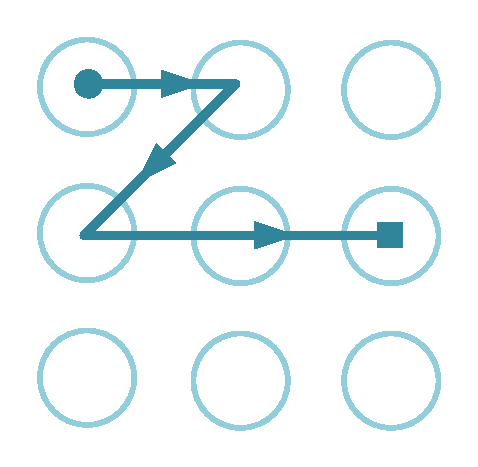
\includegraphics[width=1.3cm]{fig/611.pdf}\\
            \centering  c(2)
            \end{minipage}
        }
         \hspace{-0.2cm}
         \subfigure{
            \begin{minipage}[b]{1.3cm}
            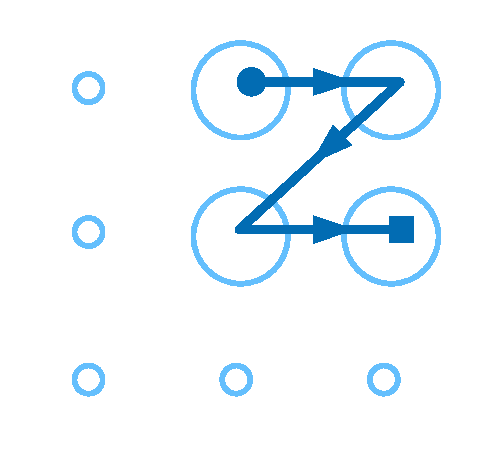
\includegraphics[width=1.3cm]{fig/612.pdf}\\
            \centering c(3)
            \end{minipage}
        }
         \hspace{-0.2cm}
         \subfigure{
            \begin{minipage}[b]{1.3cm}
            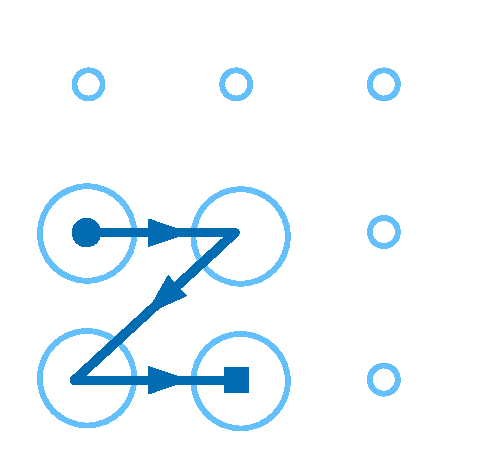
\includegraphics[width=1.3cm]{fig/613.pdf}\\
            \centering  c(4)
            \end{minipage}
        }
         \hspace{-0.2cm}
         \subfigure{
            \begin{minipage}[b]{1.3cm}
            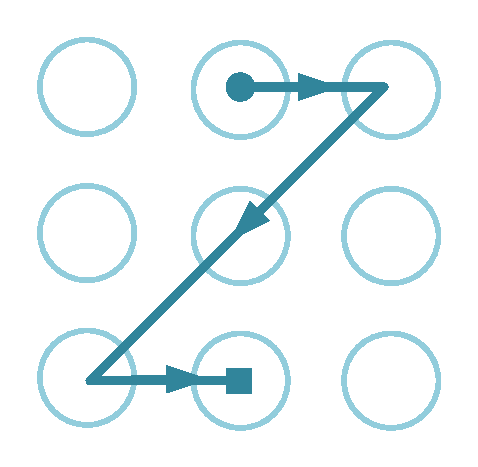
\includegraphics[width=1.3cm]{fig/614.pdf}\\
            \centering  c(5)
            \end{minipage}
        }
         \hspace{-0.2cm}
         \subfigure{
            \begin{minipage}[b]{1.3cm}
            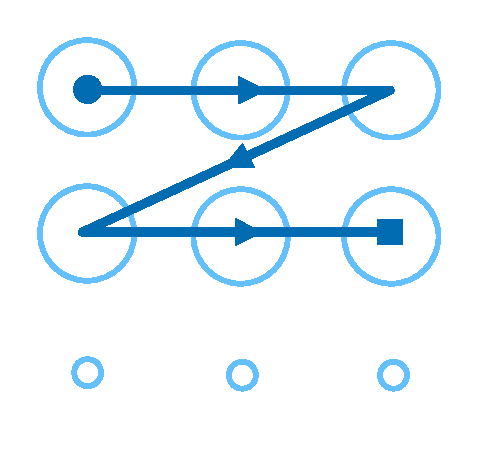
\includegraphics[width=1.3cm]{fig/615.pdf}\\
            \centering  d(1)
            \end{minipage}
        }
        \hspace{-0.2cm}
         \subfigure{
            \begin{minipage}[b]{1.3cm}
            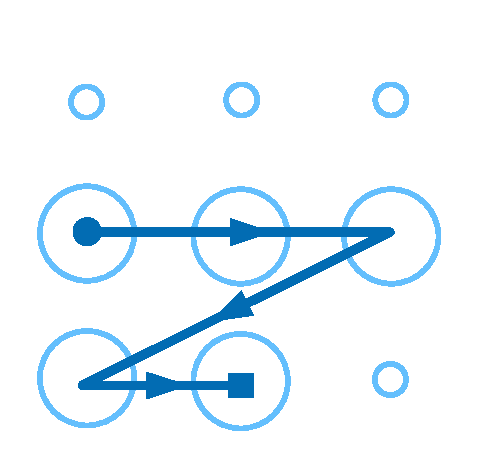
\includegraphics[width=1.3cm]{fig/616.pdf}\\
            \centering  d(2)
            \end{minipage}
        }
        \hspace{-0.2cm}
         \subfigure{
            \begin{minipage}[b]{1.3cm}
            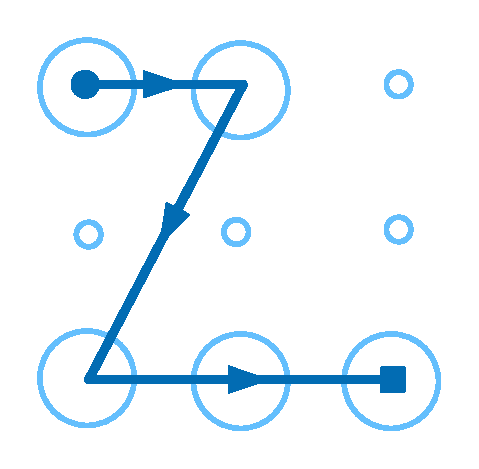
\includegraphics[width=1.3cm]{fig/617.pdf}\\
            \centering  d(3)
            \end{minipage}
        }
        \hspace{-0.2cm}
         \subfigure{
            \begin{minipage}[b]{1.3cm}
            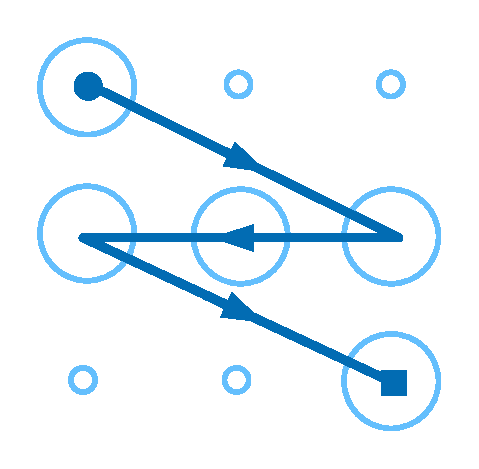
\includegraphics[width=1.3cm]{fig/618.pdf}\\
            \centering  d(4)
            \end{minipage}
        }
        \hspace{-0.2cm}
         \subfigure{
            \begin{minipage}[b]{1.3cm}
            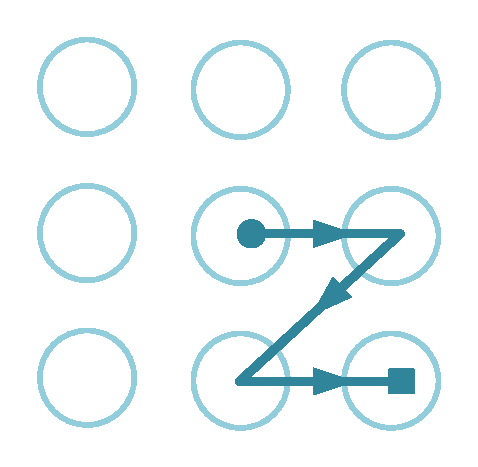
\includegraphics[width=1.3cm]{fig/619.pdf}\\
            \centering  d(5)
            \end{minipage}
        }
        \vspace{-2mm}
        \caption{Possible mappings for the tracked fingertip movement trajectory presented in Figure~\ref{fig:fig2} (d). }
        \vspace{-2mm}
        \label{fig:fig3}
    \end{figure}

    \subsubsection{Map the Tracked Trajectory to Candidate Patterns\label{section:identity}}
       In this step, we use the extracted geometry information to map the fingertip movement trajectory to a small number of candidate patterns which will then be ranked using a heuristic. This process is described in Algorithm~\ref{alg:alg1}.

        \vspace{2mm}
       \noindent \textbf{Identify Candidate Patterns.} Our implementation simply enumerates all possible
        patterns for a given pattern grid to identify candidate patterns, starting from the top-left touch point.
        We reject patterns that do not meet the requirements that the correct pattern is expected to have. The requirements are the number of line segments (this is checked by counting the number of turning points), and the length and the direction for each
        line segment.
        This is an \emph{automatic} process performed by our software system without any user involvement.
       We consider two line segments having the same length and slope if the difference between them is less
       than a threshold. Specifically, the relative length threshold, $lengthTh$, is set to 1.12 and the slope threshold, $directionTh$, is set to 0.25.
       To determine the thresholds, we have evaluated a range of possible values in our initial design experiments to choose the best performing values.

       \vspace{2mm}
       \noindent \emph{Example:} We use the pattern depicted in Figure~\ref{fig:fig2} as an example to
       describe our algorithm. Figure~\ref{fig:fig3} gives several
       possible mappings for the fingertip movement trajectory shown in Figure~\ref{fig:fig2} (d). For this particular trajectory, the collections of lengths and directions are
       $L=\{l, \sqrt{2}l, l\}$ and $D=\{5, 11, 5\}$ respectively. Any pattern that does not meet $L$ or $D$ should not be considered as a candidate pattern for this trajectory.
       For this reason, Figure~\ref{fig:fig3} a(1)--a(5) will be rejected. Take Figure~\ref{fig:fig3} a(1) as an example,
       the line lengths and directions for all four line segments of this pattern are  $\{l,
       \frac{\sqrt{5}}{2}l, l\}$ and $\{5,12,5\}$ respectively. It does not meet the expected $L$ or $D$ and should be rejected.
       The patterns presented in b(1)--b(5) and c(1)--c(5) of Figure~\ref{fig:fig3}) will
       also be rejected for the same reason.

\begin{figure}[!t]
    \centering
    \subfigure{
        \begin{minipage}[t]{0.11\textwidth}
            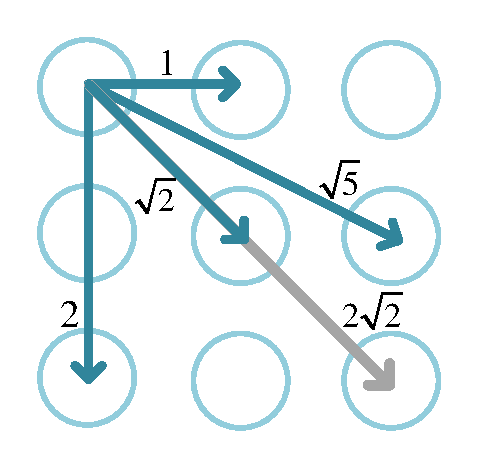
\includegraphics[width=\textwidth]{fig/physical_length.pdf}\\
            \centering  (a) line length
        \end{minipage}
    }
    \hspace{0.1cm}
    \subfigure{
        \begin{minipage}[t]{0.11\textwidth}
            \includegraphics[width=\textwidth]{fig/intersection.pdf}\\
            \centering  (b) line intersection
        \end{minipage}
    }
    \hspace{0.1cm}
    \subfigure{
        \begin{minipage}[t]{0.11\textwidth}
            \includegraphics[width=\textwidth]{fig/overlap.pdf}\\
            \centering  (c) overlapping lines
        \end{minipage}
    }
    \caption{Illustrations of the terminologies used in Equation~\ref{equ:compscore}.}
    \label{fig:intersection-overlap}
\end{figure}
\begin{figure}[!t]
            \centering
            \subfigure{
                \begin{minipage}[b]{8cm}
                \includegraphics[width=1.3cm]{fig/9-1.pdf}
                \hspace{0.1cm}
                \includegraphics[width=1.3cm]{fig/9-2.pdf}
                \hspace{0.1cm}
                \includegraphics[width=1.3cm]{fig/9-3.pdf}
                \hspace{0.1cm}
                \includegraphics[width=1.3cm]{fig/9-4.pdf}
                \hspace{0.1cm}
                \includegraphics[width=1.3cm]{fig/9-5.pdf}\\
                \centering  (a) Example patterns belong to the simple category.
                \end{minipage}
            }
            \subfigure{
                \begin{minipage}[b]{8cm}
                \includegraphics[width=1.3cm]{fig/9-6.pdf}
                \hspace{0.1cm}
                \includegraphics[width=1.3cm]{fig/9-7.pdf}
                \hspace{0.1cm}
                \includegraphics[width=1.3cm]{fig/9-8.pdf}
                \hspace{0.1cm}
                \includegraphics[width=1.3cm]{fig/9-9.pdf}
                \hspace{0.1cm}
                \includegraphics[width=1.3cm]{fig/9-10.pdf}\\
                \centering  (b) Example patterns belong to the median category.
                \end{minipage}
            }
            \subfigure{
                \begin{minipage}[b]{8cm}
                \includegraphics[width=1.3cm]{fig/9-11.pdf}
                \hspace{0.1cm}
                \includegraphics[width=1.3cm]{fig/9-12.pdf}
                \hspace{0.1cm}
                \includegraphics[width=1.3cm]{fig/9-13.pdf}
                \hspace{0.1cm}
                \includegraphics[width=1.3cm]{fig/9-14.pdf}
                \hspace{0.1cm}
                \includegraphics[width=1.3cm]{fig/9-15.pdf}\\
                \centering  (c) Example patterns belong to the complex category.
                \end{minipage}
            }
            \caption{Examples of patterns collected from our participants. Patterns are grouped into \emph{simple}, \emph{median} and \emph{complex} categories, according to their complexity scores. }
            \label{fig:fig8}
            \vspace{-3mm}
        \end{figure}

        \begin{figure}[!t]
            \centering
            \subfigure{
                \begin{minipage}[b]{0.12\textwidth}
                \includegraphics[width=\textwidth]{fig/complex3.pdf} \\
                \centering  complexity score: $43.8$
                \end{minipage}
            }
            \subfigure{
                \begin{minipage}[b]{0.12\textwidth}
                \includegraphics[width=\textwidth]{fig/complex2.pdf} \\
                \centering  complexity score: $44.7$
                \end{minipage}
            }
            \subfigure{
                \begin{minipage}[b]{0.12\textwidth}
                \includegraphics[width=\textwidth]{fig/complex1.pdf} \\
                \centering  complexity score: $46.8$
                \end{minipage}
            }
            \vspace{-2mm}
            \caption{Three most complex patterns on a $3\times 3$ grid based on Equation~\ref{equ:compscore}.}
            \vspace{-2mm}
            \label{fig:most complex patterns}
        \end{figure}


        \vspace{2mm}
        \noindent \textbf{Rank Patterns.} Candidates patterns are then ranked using a simple
        heuristic. The heuristic assumes a pattern starting from
        left dot of the grid is more likely to be the correct pattern over a
         pattern starting from a right dot. This assumption is supported
        by recent studies which show that people tend to select a left dot as the starting point
        to construct a pattern~\cite{uellenbeck2013quantifying,alpnorway}.
         If two candidate patterns
         start from the same dot, we consider the pattern with a
        longer total line length
        is more likely to be the correct pattern. Using these criteria,
        the five candidate patterns are ranked in order from subfigures d(1) to d(5) in
        Figure~\ref{fig:fig3}. Therefore, an attacker would first try the candidate
        pattern presented in Figure~\ref{fig:fig3} d(1).  This attempt will lead to a
        successful attack for the example presented in Figure~\ref{fig:fig2}. Our experimental results show that
        this heuristic is effective.





\section{Experimental Setup \label{sec:setup}}
    \subsection{Data Collection}
    \label{section:locking patterns}
    The patterns used in our evaluation were collected from users who use at least one Android device (a smartphone or a tablet) on a daily basis.
    To collect the patterns, we have distributed over 1,000 survey forms and collected back 215 valid forms, resulting in 120 unique patterns\footnote{Available to be download at: \url{https://dx.doi.org/10.17635/lancaster/researchdata/113}}.
    Our participants include 95 females and 120 males who were undergraduate or postgraduate students in our institution.
    The majority of our participants are in an age group of under 30.


    To collect the patterns, we have conducted a ``pen-and-paper" survey by asking participants to fill in an anonymized questionnaire.
    The questionnaire and survey were approved by the research ethics board (REB) of our institution.
    We have made sure that our survey complied with strict privacy regulations. For example, we did not collect any personally identifiable information other than the gender and age group of the participant. Our participants were well informed on the purpose
    of the study and how the data will be managed and used. The survey forms were distributed as voluntary homework so that the participants can take the survey form away to fill in.
     Users were invited to return the survey form anonymously within three weeks to a dedicated, locked mailbox, if they wish to participate in the study.
     To avoid a user submits multiple copies of the same form, each survey form is given a unique, randomly generated 32-digital number.


     Overall, 37.6\% of our participants confirmed that they use pattern lock as the screen lock to
     protect their Android devices on a daily basis; and 33\% of those  who do not use a pattern as their screen lock said that they
     are often required to use a pattern for authentication by an application like \texttt{Alipay}. Furthermore, 60\%
     of our participants also indicated that the pattern they provided is currently being used
     or have been used in the past by themselves. Other participants (often those did not use a locking pattern on a daily basis) indicated that they
     have provided a pattern which they would like to use if a locking
     pattern is required. Based on this information, we are confident
     that our patterns represent some of the real world
     patterns. Finally, all participants believe that a complex pattern provides stronger protection than a simple one.

        \begin{figure}[!t]
            \centering
            \includegraphics[width=0.5\textwidth]{fig/guess_prob.pdf}
            \caption{How likely a pattern can be guessed in five attempts as the complex score increases. Patterns with a complex score that is greater than 13 are
             unlikely to be guessed by an attacker within five attempts.}
            \label{fig:guessing-probability}
        \end{figure}

    \subsection{Pattern Complexity Classification}
    We quantify the complexity of a pattern using the complexity (strength) score proposed in~\cite{sun2014dissecting}.
        The complexity score, $CS_{P}$, of a pattern, $P$, is defined as:
    \begin{equation}
      CS_{P}=S_{P}\times\log_{2}(L_{P}+I_{P}+O_{P})
    \label{equ:compscore}
    \end{equation}
    where $S_{P}$ is the number of connected dots, $L_{P}$ is the the total length of all line segments that form the pattern (see Figure~\ref{fig:intersection-overlap}~a), $I_{P}$ are the number of intersections (which are also termed as ``knight moves" in some prior work~\cite{vonZezschwitz:2015:EDB:2702123.2702202}, see Figure~\ref{fig:intersection-overlap}~b) and $O_{P}$ are the number of overlapping linear segments (see Figure~\ref{fig:intersection-overlap}~c).  To calculate the line length, we assume the length between two horizontally or vertically adjunct dots is one. Thus, our method is independent of the size of the screen and the grid.


    Intuitively, the more connected dots ($S_{P}$), line segments ($L_{P}$),
    intersections ($I_{P}$) and overlapping line segments ($O_{P}$) that a
    pattern has, the more complex it is. For example, the patterns shown in
    Figure~\ref{fig:fig8} (c) use all the nine dots of the grid, and have  at
    least seven line segments and three intersections.
    There are other methods to quantify the complexity score of pattern locks, including the methods proposed by Song \emph{et al.} ~\cite{Song2015On} and Andriotis \emph{et al.}
    ~\cite{Andriotis2014Complexity}. These methods in general suggest that patterns with more connected dots and intersections are considered to provide stronger security strengths~\cite{Heidt2016Refining}.


    Figure~\ref{fig:guessing-probability} illustrates how the guessing probability\footnote{A guessing probability is
    how likely an attacker can successful guess a given pattern within five attempts.} changes as the complexity score (given by Equation~\ref{equ:compscore}) of the pattern lock changes.
    The probability is calculated on the set of patterns collected from our participants, by using the pattern strength
    measurement method proposed in \cite{Heidt2016Refining}. As can be seen from this diagram, \FIXME{explain
    the diagram – e.g. what are primitive curve and logistic fit!}.

    \vspace{2mm}
    \noindent \textbf{Pattern Grouping.}
    Base on the complexity score, we divide the collected patterns into three complexity categories: \emph{simple}, \emph{median} and \emph{complex}. A simple pattern has a score of less than 19,
    a median
    complex pattern has a score between 19 and 33, and a complex pattern must have a score greater than 33. This classification gives us roughly 40 patterns per
    category. Figure~\ref{fig:fig8} gives some examples for each category while Figure~\ref{fig:pattern-strength} shows the distribution of these patterns according to their complexity scores.
    Based on this definition, the most complex pattern on a $3 \times 3$ grid has a score of $46.8$ (see Figure~\ref{fig:most complex patterns}).  The complex scores of the patterns we collected range from $6.4$ to $46.8$.

        \begin{figure}[!t]
            \centering
            \includegraphics[width=0.5\textwidth]{fig/pattern-strength.pdf}
            \caption{The distribution of complexity scores for the patterns given by our participants.}
            \label{fig:pattern-strength}
        \end{figure}

    \begin{table}[!t]
            \centering
            \caption{Screen sizes for the test phones}
            \label{tab:locking-screen-size}
            \small
            \begin{tabular}{cccc}
                %\includegraphics[width=7.5cm]{fig/table1.pdf}
                \toprule
                \textbf{Screen size} & \textbf{MI4} & \textbf{Honor7} & \textbf{Note4} \\
                \midrule
                Height(cm)$\times$Width(cm) & $13.9\times6.9$ & $14.3\times7.2$ & $15.4\times7.9$ \\
                \bottomrule
            \end{tabular}
            %\vspace{-4mm}
    \end{table}

    \subsection{Video Recording and Preprocessing}
    \noindent\textbf{Recording Devices.} We used three smartphones for video recording: an Apple iPhone4S,
     a Xiaomi MI4 and a Meizu2 phones. Each mobile phone was used to record 40 patterns with a
    1080p HD resolution of 30 FPS under different settings.

    \vspace{2mm}
    \noindent\textbf{User Participation.} We recruited ten postgraduate students (five male and five female
    students) from our institution to reproduce the 120 patterns (collected from the users)
    and the 60 most complex patterns (see Section~\ref{sec:overall_rate})  on three target mobile phones:
    a Xiaomi MI4, a Huawei Honor7 and a Samsung Note4 smartphones. Table~\ref{tab:locking-screen-size} lists
    the screen size for each target mobile phone.

    \vspace{2mm}
   \noindent\textbf{Video Recording Setup.}
    By default, we used the  Android $3 \times 3$ native pattern grid,
    but we evaluated our approach using other pattern grids with different sizes in
    Section~\ref{sec:scalability}. We recorded each pattern under three filming
    angles, 45, 90 and 135 degrees, by placing the camera on the left-front, front, and right-front
    of the target device respectively.
    By default, the video
    was recorded indoor during daytime under a natural lighting condition. In
    Section~\ref{sec:light} we evaluated our approach under different lighting conditions
    both indoor and outdoor. By default, videos were recorded at a distance of
    2 meters from the target device and we evaluated the impact of the filming distance in
    Section~\ref{sec:scalability}.

    \vspace{2mm}
    \noindent \textbf{Video Filming.}
     Before recording, our participants were given the opportunity to practice a pattern
    several times, so that they can draw the pattern at
    their natural speed. On average, this practice session took 10 trails per user per pattern.
    When drawing the
    pattern, some participants sat, while others stood, some hold the device
    by hands, while others placed it on a table.
    Each pattern was drawn on three target devices and
    recorded under three filming angles. Thus, for the 120 patterns collected from users, we recorded 1,080 videos in total.

    \vspace{2mm}
    \noindent\textbf{Video Preprocessing.}
    For each video stream, we used the algorithm described in Section~\ref{sec:identify} to cut out the video segment
    of the unlocking process. We left around 200 to 300 milliseconds of the video segment before and after the pattern unlocking process.
    To track the fingertip locations,
    we used Windows Movie Make to highlight two areas of interest on the first frame of
    the video segment: one area surrounds the fingertip, and the other contains an edge of the
    phone (see Section~\ref {secction:shake}).

    \vspace{2mm}
   \noindent\textbf{Implementation.} Our prototyped attacking system built upon a TLD library~\cite{TLD-toolbox-web}.
    The developed software ran on an Intel Core i5 PC with
    8GB RAM. The operating system is Windows 10. Our implementation can be ported onto
    Android or Apple iOS systems, which is our future work. On our evaluation
    platform, our software takes less than 30 seconds to process a video to produce candidate patterns.

\section{Experimental Results}
    In this section, we first present the overall success rate for cracking
    the 120 patterns collected from our participants plus the top 60 most complex patterns
    on a $3\times3$ pattern grid.
    Our results show that our approach can successfully crack over 95\% of the
    patterns using no more than five attempts. We then analyze how the
     success rate is affected by the filming distance, filming angles and
    camera shake. Finally, we demonstrate that direct observations lead to poor
    performance before evaluating our approach on alternative pattern grids.

\begin{figure}[!t]
    \centering
    \includegraphics[width=0.35\textwidth]{fig/10.pdf}
    \vspace{-3mm}
    \caption{For each pattern category, the figure shows the success rate using no more than 1, 2, 3, 4 and 5 attempts.}
    \label{fig:fig10}
    \vspace{-2mm}
\end{figure}

    \subsection{Overall Success Rate \label{sec:overall_rate}}

    \noindent \textbf{Result 1:}  \emph{We can successfully crack over 95\% of the patterns in five attempts and complex patterns are less secure compared to simple patterns under our attack.}

        In this experiment, videos were recorded from a distance of 2 meters away
        from the target device. This mimics a scenario where the adversary sits
        at the next table to the user in a public space (e.g. a restaurant).
        The smartphones used for filming in this experiment were hand-held.
        Figure~\ref{fig:fig10}
        shows the success rate for cracking different types of patterns within 1, 2, 3, 4 and 5 attempts.     For all the patterns used in this evaluation,
        our approach does not generate more than  five candidate patterns.
        For complex patterns, we are able to crack all except one in the first attempt.
        For simple and median patterns, the success rate increases with more tries.
        In one attempt, we are able to
        successfully crack 60\% and 87.5\% of the simple and median patterns respectively. With two attempts, the success rate increases to 87.5\%,
        and 95\% for simple and median patterns
        respectively. Using five attempts, we are able to
        crack all simple patterns and all but one median patterns.
       The reason that we failed on one median and one complex patterns is because of some blur motions of the video footage (probably
       caused by the video compressing algorithm), which leads
       to many tracking failures. But we are able to crack the same
       pattern using a video filmed by a different device.
        It is important to note that the Android OS will not lock the device unless seeing
        more than five failed tries~\cite{egelman2014you}. This means, in practice, our approach is able to
        successfully crack most locking patterns.

\begin{figure}[!t]
    \centering
    \includegraphics[width=0.35\textwidth]{fig/11.pdf}
    \vspace{-3mm}
    \caption{The distribution of candidate patterns for each category. No more than 5 candidate patterns were generated by our algorithm. }
    \label{fig:fig11}
    \vspace{-2mm}
\end{figure}

        Another interesting observation is that in contrast to many people's
        intuition, complex patterns do not provide stronger protection under our attack because
        most of these patterns can be cracked in one attempt.
        This is because although complex patterns can better protect the user against direct observation techniques like shoulder surfing~\cite{shoulder}, their unique graphical structures
        often allow our system to reject most patterns to produce a single candidate pattern. This is
        confirmed by Figure~\ref{fig:fig11}. It shows that for most median and all complex patterns, our system produces one candidate pattern --
        the correct one for most of our test cases.


       We also evaluated our approach using the top 60 most complex
        patterns (according to Equation~\ref {equ:compscore}) on a $3 \times 3$
        grid.
        To evaluate our approach on a wide range of patterns, we exclude patterns that are simply a rotation to an already chosen pattern.
         Figure~\ref {fig:most complex patterns} illustrates three
        highly complex patterns which have a complexity score between 43.8 and 46.8. The three
        patterns use all the nine dots of the grid and have a larger number of line segments, intersections and overlapping lines when compared to simpler patterns.
        Because of their complex graphical structures, it would be hard to remember
        these patterns using direct observation techniques.
        In this experiment, we can crack all the complex patterns in one attempt. This result reinforces our claim that complex
        patterns are less security under video-based attacks.




    \begin{figure*}[!ht]
            \centering
            \subfigure{
                \begin{minipage}[b]{3.8cm}
                \includegraphics[width=3.8cm]{fig/distance-2m.pdf}\\
                \centering \footnotesize (a)
                \end{minipage}
            }
            \hspace{-0.1cm}
            \subfigure{
                \begin{minipage}[b]{3.8cm}
                \includegraphics[width=3.8cm]{fig/distance-3m.pdf}\\
                \centering \footnotesize (b)
                \end{minipage}
            }
            \hspace{-0.1cm}
            \subfigure{
                \begin{minipage}[b]{4cm}
                \includegraphics[width=4cm]{fig/distance-3-5m.pdf}\\
                \centering \footnotesize (c)
                \end{minipage}
            }
            \hspace{-0.1cm}
            \subfigure{
                \begin{minipage}[b]{3cm}
                \includegraphics[width=3cm]{fig/distance-pattern.pdf}\\
                \centering \footnotesize (d)
                \end{minipage}
            }
                \vspace{-3mm}
            \caption{Tracked fingertip trajectories (user's perspective) for the pattern shown in (d) from a video filmed from a distance of 2m (a), 3m (b), and 3.5m (c) respectively away from the target device. The tracking quality decreases when the filming distance is greater than 3m. }
            \vspace{-3mm}
            \label{fig:distance-show}
        \end{figure*}



    \subsection{Impact of Filming Distances \label{sec:distances}}
        \begin{table}[!t]
            \centering
            \caption{Tracking precision vs filming distance}
            \vspace{-0.2mm}
            \label{tab:tab1}
            \small
            \begin{tabular}{ccccc}
                \toprule
                \textbf{Distance}& 1 m & 2 m & 3 m & 3.5 m \\
                \midrule
                \textbf{fingertip}  & 100\% & 98.7\% & 80.9\% & 68\% \\
                \textbf{device edge} & 100\% & 99.4\% & 90.6\% & 69\% \\
                \bottomrule
            \end{tabular}
            \vspace{-5mm}
        \end{table}


        \noindent \textbf{Result 2:} \emph{We can crack over 80\% of the patterns in five attempts, if the video was filmed using a smartphone within a distance of 2.5 meters away from the target.}

           We would like to know how the filming distance affects the
           success rate of the attack. To do so, we have asked our participants to randomly select all 120
           pattern locks and we varied the
           filming distance from 1 meter to 3.5 meters.
           Figure~\ref{fig:fig12} shows how the cracking success rate changes
           as the filming distance increases. There is slight differences in the success rate between this diagram and Figure~\ref{fig:fig10}
            because we used less patterns in this experiment.
           When the filming distance is less than 2 meters, our approach can crack all patterns in five attempts.
           The success rate drops significantly when
           the filming distance is greater than 2.5 meters.
           The quality of the video filmed by a mobile phone tends to drop significantly with many object deformations. The degradation of the video quality makes it difficult for the TLD algorithm to successfully track objects across video frames.
            This is confirmed by Table~\ref{tab:tab1}
           which shows that the tracking precision for the fingertip and the device edge drops from around 99\% to
           68\% when the filming
           distance increases from 2 meters to 3.5 meters. The increased
           tracking failures result in an increased number of missing
           points on the tracked trajectory, leading to a deteriorative performance in identifying candidate patterns.
           This can be seen from Figure~\ref{fig:distance-show} where the quality
           of tracking clearly decreases when the filming distance is greater
           than 3 meters.
           Nonetheless, our approach can
           achieve a high success rate when the filming distance within
           2.5 meters. Such a distance allows an attacker to
           record the video without raising suspicions in many day-to-day scenarios (some of these are
           described in Figure~\ref{fig:fig1}).

            We also evaluated our approach on videos filmed using a Nikon D90
            single-lens reflex (SLR) camera with a 105mm lens. The SLR camera
            was placed from a distance of 9 meters away from the target
            device. For this set of videos, we are able to achieve the same
            performance when compared to using videos filmed by a mobile
            phone camera with a 2-meter filming distance. The further filming
            distance is largely due to better video quality brought by the advanced
            SLR camera and the lens. Therefore, in practice, an attacker can
            also use a professional video recording device to launch the
            attack from a further distance.


    \subsection{Impact of Camera Shake}

    \noindent \textbf{Result 3:} \emph{Our method can tolerate a certain degree of camera shake in the hand-held mode.}

    In this experiment, we used an IPhone4S smartphone to record how a pattern is drawn on a Huawei Honor7 phone. This experiment was carried out under three settings:
    \emph{fixed}, \emph{hand-held} and \emph{shaky}, where the filming
    device was respectively fixed using a tripod, hand-held, and hand-held but with constant movements of
     approximate 2cm in the horizontal or the vertical directions. The recording device was placed on the left-front, front, and right-front of the target device.
    In the experiment, we fixed the target device on a table using double-sided tapes.

    We use a reference point to quantify camera shake. The point
    is the center position of an area of the target device. The area is marked by a boundary box on the first
    frame (see Figure~\ref{fig:fig5}). We calculate the difference (in terms of pixels) for where the
    reference point was seen in two consecutive video frames. We then use the difference to measure the degree of camera shake.
    Figure~\ref{fig:fig13} shows the cumulative distribution function (CDF)
    of camera shake under the three different filming settings.
    Here, the wider the distribution is, the less steady the
     filming is. The shaky mode is least stable where the difference of the reference point between two video frames can be up to 250 pixels.


    Figure~\ref{fig:fig14} shows that our approach has the same performance under
    the hand-held and the fixed modes. The modest camera sake under the hand-held mode
    has little impact on performance thanks to our camera-shake-calibration method. We observe deteriorative performance
    under the shaky mode, but the performance degradation is modest (80\% vs 97\%
    in 5 attempts). In reality, an attacker would avoid drastic
    camera shake by firmly holding the video recording device.

        \begin{figure}[t!]
            \centering
            \includegraphics[width=0.35\textwidth]{fig/12.pdf}
            \vspace{-3mm}
            \caption{Impact of the filming distance.}
            \label{fig:fig12}
           \vspace{-3mm}
        \end{figure}

\begin{figure}[t!]
    \centering
    \includegraphics[width=0.35\textwidth]{fig/13.pdf}
    \vspace{-2mm}
    \caption{The cumulative distribution function (CDF) for different video recording modes.}
    \vspace{-2mm}
    \label{fig:fig13}
\end{figure}

\begin{figure}[!t]
    \centering
    \includegraphics[width=0.35\textwidth]{fig/14.pdf}
    \vspace{-2mm}
    \caption{Impact of camera shake. Our approach has the same success rate under the hand-held and the fixed modes and the performance degradation under the shaky mode is modest. }
    %\FIXME{We should evaluate this on 3 and 4 attempts.}
   \vspace{-2mm}
    \label{fig:fig14}
\end{figure}





    \subsection{Impact of Lighting Conditions \label{sec:light}}
    \noindent \textbf{Result 4:} \emph{Low-light has a negative impact on the success rate of the attack but our approach can still break over 70\% of the patterns when the video was filmed in a low-light environment.}

    In this experiment, videos were recorded under different lighting conditions both indoor and outdoor.
    The experimental settings are given in  Table~\ref{tab:light}.
    The light intensity of these condidtions ranges from 9500
    lux (strong light), onto 240 lux (normal light), and 55-70 lux (low light).
    These represent some of the day-to-day scenarios where filming can
    take place. For each setting, we asked each of our 10 participants to draw all collected 120 patterns on a Xiaomi MI4 phone. We used
    an iPhone4S phone to record the video. The filming camera was place on the
    left-front, front, and the right-front of the target device from a distance
    of 2 meters.


    Figure~\ref{fig:light} shows that the success rate increases when video filming were performed in a brighter lighting condition as the light intensity
    changes from 55 lux to 9500 lux. This is expected as low-light leads to
    increased video noise, blurred motion and poor focus, which all have a
    negative impact on the TLD algorithm. Nonetheless, our attack
    can still crack over 70\% of the patterns in a filming
    environment with low light.

            \begin{table}[!t]
            \centering
            \caption{Lighting Conditions}
            \label{tab:light}
            \scriptsize
            \begin{tabular}{lcccc}
                \toprule
                \textbf{Scenarios} & Indoor  & Indoor & Indoor  & Outdoor\\
                \midrule
                \textbf{Time} & nighttime &  nighttime & daytime & daytime \\
                \textbf{Light Source}& warm LED & white fluorescent & sunlight &  sunlight \\
                \textbf{Light Intensity (Lux)} & $55-70$ & $70-100$ & $150$--$240$ & $500$--$9500$ \\
                \bottomrule
            \end{tabular}
            \vspace{-2mm}
        \end{table}


       \begin{figure}[t!]
            \centering
            \includegraphics[width=0.35\textwidth]{fig/light.pdf}
            \vspace{-2mm}
            \caption{The cracking success rate within five attempts under different lighting conditions.}
            \label{fig:light}
        \end{figure}



    \subsection{Impact of Filming Angle Estimation \label{sec:angle}}
        \begin{figure}[!t]
        \centering
        \includegraphics[width=0.35\textwidth]{fig/15.pdf}
        \vspace{-2mm}
        \caption{Impact of estimation errors of filming angles.}
        \vspace{-2mm}
        \label{fig:fig15}
    \end{figure}

    \noindent \textbf{Result 5:} \emph{Our attack performs well when the error of filming angle estimation is less than 5 degrees.}

   Our approach needs to transform the tracked fingertip movement trajectory to the
   user's perspective based on an estimation of the filming angle
   (Section~\ref{sec:transformation}).
   Because our filming angle estimation
    algorithm gives highly accurate estimation, we did not find the estimation error to be a problem in our experiments.
   Nonetheless, it is worth studying how the estimation error affects the success rate of our attack. To do so, we deliberately added an error of 5-10 degrees to the estimation.

    Figure~\ref{fig:fig15} shows the results of this experiment. When the error is less than $\pm 5$ degrees, there is little impact
    on \emph{complex} patterns and no impact at all on \emph{simple} and
    \emph{median} patterns. However, an estimation error of more than 10 degrees can significantly affect the success rate.
    Given such an error, the resulted trajectory after transformations will
    be significant different from the correct pattern.
    For example, when the estimation error is 10 degrees from the
    true value,  on average, 0.8, 2.6 and 4.2 line segments per pattern respectively will
    be incorrectly labelled for \emph{simple}, \emph{median} and
    \emph{complex} patterns. This explains why the success rate for complex patterns drops significantly when there is
    an error of 10 degrees.

    \subsection{\FIXED{Impact of Different Targets and Cameras}}
    \noindent \textbf{Result 6:} \emph{The size of smartphone touch-screen and brands of mobile camera had little effect on the success rate.}

    Intuitively, the success rate may be influenced by the size of touch-screen because the length of pattern will be short as the size decreases. Likewise, the accuracy also may be influenced by the quality of video as the different quality of phone cameras. To evaluate this effection, we ask 10 participants to randomly select 60 patterns (30 patterns for each category). We use IPhone6, Xiaomi MI4, Vivo X7, Samsung Note4 to record unlock videos while the patterns are drawn on IPhone4S\footnote{Participants draw patterns on the login interface of Alipay installed on the phone as Apple operating system do not support pattern lock authentication mechanism.}, Huawei Honor7 and Samsung Galaxy Tab E. The distance is 2m away from the tester during record the unlocking process. Table~\ref{tab:screen-size} shows the sizes of touch-screen and Table~\ref{tab:camera-parameters} presents the parameters of camera used in this experiment.
    
    \FIXED{Here analyze experimental results.}

    \begin{table}[!t]
            \centering
            \caption{Touch-screen sizes for the test phones}
            \label{tab:screen-size}
            \scriptsize
            \begin{tabular}{|c|c|c|c|}
                \hline
                \diagbox[dir=SE]{Size}{Brands}& IPhone4S & Honor7 & Samsung Tab \\
                \hline
                Height(cm)$\times$Width(cm) & $11.5\times5.9$ & $14.3\times7.2$ & $24.2\times15.0$ \\
                \hline
            \end{tabular}
            %\vspace{-4mm}
    \end{table}

    \begin{table}[!t]
            \centering
            \caption{The main parameters for the phone camera}
            \label{tab:camera-parameters}
            \small
            \begin{tabular}{|c|c|c|c|c|}
                \hline
                \diagbox[dir=SE]{Parm}{Brands}& IPhone6 & Vivo X7 & MI4 & Note4 \\
                \hline
                Frame Rate (fps) & $30$ & $30$& $30$ & 30 \\
                \hline
                Pixels & 8mp & 13mp & 13mp & 16mp \\
                \hline 
                Focus (mm) & 4.15 & 4 & 4 & 4.2 \\
                \hline
                Sensitivity (ISO) & 3200 & 3200 & 3000 & 5000 \\
                \hline
            \end{tabular}
    \end{table}

    \subsection{Inferring Patterns with Eyes}

    \noindent \textbf{Result 7:} \emph{Our attacking methodology significantly outperform direct observation techniques.}

   In this experiment, we investigate whether an attacker can infer the pattern by
   simply watching the video or through direct observations. To answer this question, we asked each of our 10 participants to watch 60 videos (where
   a pattern was drawn by other participants) to guess the pattern.  We
    only played the video segment during which a pattern is drawn to the participant (around 3 seconds per video).
   To familiarize participants with the process, we
    played  five sample videos and showed the correct patterns at the end of each video to our participants before the experiment.
   Each participant then had 10 minutes to watch a video and five chances to guess a pattern. They could adjust the playing speed and
   replay the video multiple times as they wished.


        Figure~\ref{fig:look-unlocking process} (a) shows the success rate of pattern guessing with
        bare eyes. Our participants correctly guessed for nearly half of the
        simple patterns in five attempts. However, they found that it is difficult
        to infer complex patterns with many line segments, overlapping lines and intersections.
        The success rate of guessing complex patterns is less than 10\% in five attempts.
        This is not a surprising result
        because although it is possible to correctly guess patterns with
        simple structures by watching the video, doing so for patterns with
        more complex structures is much harder.


    We also asked participants to directly observe how a pattern was drawn
    from a distance of 2 meters away from the target device. The intuition
    behind this evaluation is that human eyes can catch richer information
    over a video camera. The results of this experiment are shown in
    Figure~\ref{fig:look-unlocking process} (b).  As can be seen from the
    diagram, although the success rate is improved compared to directly watching the video, the chances for guessing the correct pattern in
    5 attempts are quite low. In
    fact, the success rates are just 48.3\%, 38.3\%
    and 11.7\% respectively for simple, median and complex patterns.

        \begin{figure}[!t]
            \centering
            \subfigure{
                \begin{minipage}[t]{0.35\textwidth}
                \includegraphics[width=\textwidth]{fig/look-video.pdf}\\
                \centering \footnotesize (a) video watching
                \end{minipage}
            }
            \hspace{-0.1cm}
            \subfigure{
                \begin{minipage}[t]{0.35\textwidth}
                \includegraphics[width=\textwidth]{fig/look-finger.pdf}\\
                \centering \footnotesize (b) direct observations
                \end{minipage}
            }
            \vspace{-2mm}
            \caption{Success rates of guessing patterns through watching the video (a) or direct observations (b).}
            \label{fig:look-unlocking process}
        \end{figure}

        \begin{figure}[!t]
            \centering
            \includegraphics[width=0.35\textwidth]{fig/scalability.pdf}
            \vspace{-3mm}
            \caption{Success rates of our attack for different locking grids.}
            \vspace{-2mm}
            \label{fig:scalability}
            \vspace{-2mm}
        \end{figure}

    \subsection{Evaluation on Other Pattern Grids\label{sec:scalability}}
    \noindent \textbf{Result 8:} \emph{A pattern grid with more dots provides stronger protection but our attack can still crack most of the patterns.}

        There are a few applications (such as CyanLock) and customized ROMs available to increase the size of the pattern grid from $3\times3$ to $4\times4$, $5\times5$, and $6\times6$.
        Although a $3 \times 3$ grid remains
        a popular choice (as it is supported by the native Android OS), it is worth studying whether
        having more touch dots on a pattern grid leads to stronger security. In this
        experiment, we first ranked all possible patterns for each grid setting in
        ascending order according to their complexity scores. We then equally
        divided the patterns into three groups, simple, medium and complex,
        and asked our participants to randomly select 20 patterns from each group for evaluation. We
        report the success rate of our attack within five attempts. In the experiments, we have adapted our algorithms for each grid setting
        by adjusting the algorithm parameters (such as the line direction numbers).


        Figure~\ref{fig:scalability} shows the success rate of our attack
        for different grids. Similar to a $3 \times 3$ grid, our
        approach achieves a higher success rate for complex patterns over
        simple ones. On average, we can crack 90\% of the complex patterns.
        We observed that a grid with more dots does provide
        stronger protection. For complex patterns, the success rate of our
        attack drops from 95\% on a $4 \times 4$ grid to 87\% on a $6 \times
        6$ grid. For simple patterns, the success rate of our attack drops
        from 85\% on a $4 \times 4$ grid to 75\% on a $6 \times 6$ grid. This
        is because a fingertip trajectory can be mapped to a larger number of
        candidates on a grid with more dots. For instance, the pattern shown
        in Figure~\ref{fig:fig2} (f) can be mapped to 55
        candidate patterns on a $6 \times 6$ grid as opposite to 5 on a $3
        \times 3$ grid. Overall, our attack can crack over 75\% (up to 95\%)
        of the patterns within five attempts. One of the purposes of introducing
        pattern grids with more dots is to allow users to use more complex
        patterns. However, this experiment suggests that complex patterns remain less security on these grids under our attack.

        \begin{figure}[!t]
            \centering
            \subfigure{
                \begin{minipage}[t]{0.18\textwidth}
                \includegraphics[width=\textwidth]{fig/pattern_screen.png}\\
                \centering \footnotesize (a) pattern-based interface
                \end{minipage}
            }
            \hspace{0.5cm}
            \subfigure{
                \begin{minipage}[t]{0.18\textwidth}
                \includegraphics[width=\textwidth]{fig/pin_screen.png}\\
                \centering \footnotesize (b) pin-based interface
                \end{minipage}
            }
            \caption{Pattern-based and pin-based authentication interfaces from Xiaomi MI4 phone.}
            \label{fig:unlock interface}
        \end{figure}

    \subsection{\FIXED{Evaluation of Cracking PIN-based Passwords}}
        \noindent \textbf{Result 9:} \emph{PIN-based passwords are still vulnerable under our attack. This can be proved that we can break over {\color{red}90\%} of the passwords using simple a variant of our attacking method.}
        
        Recall the basic idea of our attack, pattern lock can be reconstructed by tracking the fingertip movement  from the target video. Intuitively, out method can also infer to the PIN-base passwords by analyzing the pattern which is generated during unlocking the device. To prove this intuitively imagine, we total collected 60 PIN-based passwords which were separated into two categories: 4-digital and 6-digital passwords and the number of each category is 30. For each category, we ask our participants to keystroke the passwords on a Xiaomi MI4 phone. Figure~\ref{fig:unlock interface} shows the pattern-based and pin-based authentication interface of MI4 phone.  We use an IPhone4S phone to record the video respectively on the left-front, front and right-front of the target device from a distance of 2 meters.
        
        \noindent \textbf{Variant Methodology} There exists some differences between PIN-based passwords and pattern lock. These are summarized as follow: (1) PIN-base authentication interface has ten dots that is different from pattern lock, making the layout of interface of the two mechanisms different; (2) the dots on PIN-based interface can be typed repeated while they can only be visited once on pattern-base interface. The above differences make the patterns generated from the two authentication mechanisms significant different.  To this point, we increased the geometric information including both direction and length information to adjust the variant attack method for reconstructing PIN-base passwords.
        
        \FIXED{Here show the experimental results.}
        
        
    
\section{Discussions}

\subsection{Potential Countermeasures}

The success of our attack depends on three factors: (1)
knowledge of the pattern grid; (2) a decent
quality video footage allowing the algorithm to track the fingertip movement;
(3) successfully identifying a video segment that captures the entire process of pattern drawing.


For the first factor, the attacker can obtain relevant information via analyzing a device installed with the same operating system and applications as the target.
Randomization techniques such as 
randomized pictures~\cite{biddle2012graphical,hossein2015fortifying} could be a solution for the first factor.
However, randomization-based solutions often come at the cost of poorer
usability. This can prevent them to be used at a large scale.
Regarding the second factor, there are ways, such as
KALEIDO~\cite{zhang2015kaleido}, to prevent unauthorized videotaping by
dynamically changing the colour and brightness of the screen to confuse the
filming camera. A non-technical solution for this aspect would be to educate users to
fully cover their fingers when drawing a pattern. But doing this on a large-screen device could be awkward especially when the device is held by one hand.
For the third factor, the attacker's solution depends on the type of the pattern. For a screen lock, pattern drawing is the first activity (except
for receiving a phone call or making an emergency call) when the device is
retrieved. Therefore, identifying the video segment is straightforward. When
the pattern is used by applications, we have observed that users typically
pause for a few seconds before or after entering the pattern. Therefore, an experienced attacker should also be able
to identify the video segment in case our automatic algorithm (presented in
Section~\ref{sec:identify}) fails to do so. A potential countermeasure is to mix 
pattern unlocking with other on-screen activities. For examples, before and
after pattern drawing, the system can ask the user to type in a sentence
using a Swype-like method or
to draw some graphical shapes. The problem of this approach is it may annoy users by asking 
them to do more, especially for screen unlocking -- an activity that is performed 
many times a day.

%De Luca \emph{et. al} proposed a new touch screen authentication using both the pattern and the touch screen data(pressure, time, speed, etc.)~\cite{de2012touch}, However, this design decreases the usability of


\subsection{Implications}
While pattern lock is preferable by many users~\cite{androidstudy}, this     work shows
that it is vulnerable under video-based attacks. Our attack
is able to break most patterns in five attempts. Considering Android
allows five failed attempts before automatically locking the device, our work
shows that this default threshold is unsafe. We demonstrated that, in contrast to many users'
perception, complex patterns actually do not provide stronger protection over simple patterns under our attack.

It is worth mentioning that our approach is only one of the many attacking
methods that researchers have demonstrated. Examples of these attacks include
video-based attacks on keystroke-based authentication~\cite{shukla2014beware,yue2014blind}, sensor-based attacks for
pattern lock~\cite{zhang2016privacy}. Authentication methods that combine different
authentication methods~\cite{de2012touch,stefan2012robustness,lingsecure,mannan2007using} to constantly checks the user's identity could be
a solution. %However, due to stealthiness and diversity of
%such attacks, there may not exist an ``one-size-fits-all" solution.



   % \FIXED{In this section, we discuss some possible defense strategies against video-based attacks proposed in this paper. For other attack approaches introduced in related work, there are some other defense strategies. In order to protect the text-based passwords, randomized keyboard \cite{hoanca2005screen,shin2010device,kim2012keypad}have been proposed against computer vision based attacks.}
%
%    \FIXED{Indeed, there are also some other authentication approaches immune to video-based attack. With the widely use of various diversity of sensors embed into smartphones, Shahzad \cite{shahzad2013secure} propose a protection approach by multiple information collected by sensor such as gyroscope and accelerator. This defense approach, unfortunately, seems to be attacked by Serwadda \cite{serwadda2013kids}, who proposed a new attack method for multi-authenticated information produced by sensors. In addition, biometric-rich locking mechanisms have been proposed \cite{kalal2012tracking,hoanca2005screen}. The successful use of fingerprint authentication on iPhone is a positive example for preventing the video-based attack. But recently researcher points that fingerprint can be forged~\cite{shin2009dictionary}, making the fingerprint authentication mechanism is also unsafe.}
%
%    \FIXED{To prevent the video from filming secretly, Lan Z proposes the KALEIDO~\cite{zhang2015kaleido}, a system that prevents unauthorized users from recording a high-quality redisplay on a screen by taking full use of light difference between the screen-eye channel and the screen-camera channel. Thus, in our further work, based on such limited disparities, we can design a system that prevent the attacker from implementing video-based attacks. Specifically, to obstruct the video filming, the certain frequency of light can be launched by touch-screen during drawing the pattern lock.}
%
%    \FIXED{With the advent of new technologies, however, there are still some novel attack methods arouse. Due to stealthiness and diversity of such attacks. There are not a uniform countermeasure to protect our private data from leakage. The best approach for protecting privacy is enhance safety consciousness and if possible, do not input your private information in public places.}

\section{Related Work}
\label{section: relate-work}
Our work lies at the intersection between computer vision based attacks and
cracking graphical- and touch-based authentication methods. This work brings
together techniques developed in the domain of computer vision and motion
tracking to develop a new attack. Our work is the first attempt
of reconstructing a locking pattern from a video footage without
capturing the content displayed on the screen.

\vspace{2mm}
\noindent \textbf{Computer Vision-based Attacks} No work has targeted using video
footage to crack Android pattern lock and this is the first to do so. Our work is inspired by the work
presented by Shukla \emph{et al.}~\cite{shukla2014beware} on video-based attacks of
PIN-based passwords. In addition to addressing the new challenges highlighted in Section~\ref{sec:intro}, our work differs to their approach in
two ways.
Firstly, we target a different authentication method, i.e. graphical-based passwords are fundamentally different from PIN-based passwords. %Secondly, we
%exploit the geometry information exposed by fingertip movement to identify candidate patterns.
Secondly, our approach does not require knowledge of the size of the screen or the grid.
Other work in the area including~\cite{yue2014blind} which attacks PIN-based passwords by analyzing how the screen brightness changes when entering a password.
But the subtle changes of the screen brightness can be dramatically affected by the lighting condition. This restricts the application of their approach.
There is a body of work using reflections to recover information typed by the user~\cite{kuhn2002compromising,xu2013seeing,raguram2011ispy,backes2009tempest}. These schemes require having a clear vision of the content displayed on the screen while our approach does not have such a requirement.

\vspace{2mm}
\noindent \textbf{Cracking Graphical-based Passwords.}
Aviv \emph{et al.} demonstrated that it is possible to reconstruct a locking pattern by analyzing the oily residues left on the screen~\cite{aviv2010smudge}.
 This method is highly restricted as oily residues can be messed up by any on-screen activities after pattern drawing.
Zhang \emph{et al.} exploit the WiFi signal interferences caused by finger motions to recover patterns~\cite{zhang2016privacy}. Their method requires a complex setup and is highly sensitive to moving objects of the environment
because the WiFI signal can be disrupted by a moving object.

\vspace{2mm}
\noindent \textbf{Attacks on Touch-based Authentication.}
%\FIXME{See: When Kids' Toys Breach Mobile Phone Security, CCS 13 and other papers}
Ballard \emph{et al.} implemented a forgery attack on handwriting
authentication~\cite{ballard2007forgery}. Using a small number of training
examples, they achieve a high success rate for this attack. More recently,
Serwadda \emph{et al.} show that a simple robot can achieve high penetration
rates against touch-based authentication systems by analyzing on-screen gestures including
swiping and zooming~\cite{serwadda2013kids}.
In this paper, we present a new, video-based attack for graphical-based passwords.
Research in this area all demonstrates the need for a closer look of the security risks of touch-based authentication.


\vspace{2mm}
\noindent \textbf{Study of Android Pattern Lock.}
Uellebenk \emph{et al.} study how people use Android pattern lock on
a daily basis~\cite{uellenbeck2013quantifying}.  They found that although there
is a large number of Android patterns, in
practice many people only use a small set of them due to users' bias in
generating patterns. L{\o}ge explored the correlation between
human's characteristics (e.g. ages and genders) and the choice of
patterns~\cite{alpnorway}. Her study shows that users have a bias in selecting the
starting dot to form a pattern and people tend to use complex patterns
for sensitive applications.
Aviv \emph{et al.} conducted a large user study to understand the security of the Android graphical based passwords~\cite{Aviv2014Understanding}. They analyzed the security and usability preference of users, using six visual features of the pattern lock including pattern length, number of crosses, etc.
Based on this study, they developed a brutal-force  algorithm to
crack the pattern lock~\cite{Aviv2015Is}. Their results show that patterns
generated on a grid of $3\times3$ and $4\times4$ dots can be cracked
within thousands of guesses, where simple patterns need less
attempts. In a more recent work~\cite{Aviv2016Anlyzing}, they study the representativeness of
pattern locks collected through various methods. Their work suggests
that there are subtle differences for patterns collected using a pen-and-paper
 and online survey.

\vspace{2mm}
\noindent \textbf{Motion Tracking.} In addition to TLD, there are other methods proposed in the past for tracking object
motions. Some of them apply image analysis to track the hand and gesture
motions from video
footage~\cite{Yang:2002:EMT:605089.605095,Stenger:2006:MHT:1159166.1159342,
Beh2014Rule}. In this paper we do not seek to advance the field of
motion tracking. Instead we demonstrate that a new attack can be built
using classical motion tracking algorithms. We show that the attack presented in
this work can be a serious threat for Android pattern lock. %This has never been attempted in
%prior work on motion tracking.

\section{Conclusions}
This paper has presented a novel video-based side-channel attack for
Android pattern lock. The attack is based on a video filmed a distance of 2 meters away from the target device using a mobile phone camera. The attack is
achieved by employing a computer vision algorithm to track the
fingertip movement from the video, and then using the geometry information
of the fingertip movement trajectory to identify the most likely patterns to be
tested on the target device.  Our approach was evaluated using 120 unique patterns collected
from independent users and some of the most complex patterns. The experimental results show that our approach
is able to successfully crack over 95\% of the patterns in five attempts.
We show that, in contrast to many people's belief, complex pattern actually provides
weaker protection over simple patterns under our attack. Our study
suggests that Android pattern lock is vulnerable to video-based
side-channel attacks.

    %\FIXED{In this paper, we present a novel computer vision based attack that cracks the Android locking patterns based on a video that is unnoticeably filed from a certain angle. Our attacking method uses a video tracking algorithm to track the fingertip motion trajectory, and then outputs a small number of candidate pattern locks by analyzing the line segments and their angle of the fingertip motion.}
%
%    \FIXED{To evaluate this attacking approach, we collect 600 patterns from 215 independent users by asking them to fill an anonymized questionnaires and select 120 unique patterns after removing identical ones for performing various experiments. The experimental results shows that the attack system can unlock the target phone with a success rate of above 95\% with no more than five attempts -- a default threshold when the phone will automatically locked by the Android operating system. Furthermore, this work shows that a complex pattern lock is easier to be cracked than a simple one, a great contradiction in most people's mind that a complex pattern lock is more secure than a simple one. At last, we propose a new insights on how to design and use a pattern lock system in a secure way.}
%
%    %In this paper, we present a novel computer vision based attack that cracks the pattern locks with the unnoticeably filmed video. In this attack, first we film the video from a certain angle. Then we leverages the fingertip movement during the pattern entry process to analyze pattern locks. In order to correct the video filming angles, we use the transformation matrix to map the movement to the victim's perspective. To exclude the similar patterns, we propose a novel representation for pattern locks by graphic knowledge. We implement a prototype of the attack and evaluate it with lots of videos filmed in various situations. The empirical results indicate that we can achieve an average accuracy of 95\% within five trials at two meters away from the touch-screen.
%
%    %However, this attack also exists some limitations which are as following. If user cover his finger during drawing the pattern lock, the accuracy of this attack will be very low and even fails to recognize the pattern lock. Indeed, with the distance increasing, the accuracy will decrease rapidly. Further, when the distance is greater than 3m, the accuracy will be very low. This above limitations is also our future work. Next we will continue on focusing our attention on this limitation and making the attack more robust.



\IEEEpeerreviewmaketitle


\ifCLASSOPTIONcaptionsoff
  \newpage
\fi



\bibliographystyle{IEEEtranS}
\balance
\bibliography{refs}

% that's all folks
\end{document}


